% -*- mode: Latex; fill-column: 120; -*-
\documentclass{article}\usepackage[]{graphicx}\usepackage[]{color}
%% maxwidth is the original width if it is less than linewidth
%% otherwise use linewidth (to make sure the graphics do not exceed the margin)
\makeatletter
\def\maxwidth{ %
  \ifdim\Gin@nat@width>\linewidth
    \linewidth
  \else
    \Gin@nat@width
  \fi
}
\makeatother

\definecolor{fgcolor}{rgb}{0.345, 0.345, 0.345}
\newcommand{\hlnum}[1]{\textcolor[rgb]{0.686,0.059,0.569}{#1}}%
\newcommand{\hlstr}[1]{\textcolor[rgb]{0.192,0.494,0.8}{#1}}%
\newcommand{\hlcom}[1]{\textcolor[rgb]{0.678,0.584,0.686}{\textit{#1}}}%
\newcommand{\hlopt}[1]{\textcolor[rgb]{0,0,0}{#1}}%
\newcommand{\hlstd}[1]{\textcolor[rgb]{0.345,0.345,0.345}{#1}}%
\newcommand{\hlkwa}[1]{\textcolor[rgb]{0.161,0.373,0.58}{\textbf{#1}}}%
\newcommand{\hlkwb}[1]{\textcolor[rgb]{0.69,0.353,0.396}{#1}}%
\newcommand{\hlkwc}[1]{\textcolor[rgb]{0.333,0.667,0.333}{#1}}%
\newcommand{\hlkwd}[1]{\textcolor[rgb]{0.737,0.353,0.396}{\textbf{#1}}}%
\let\hlipl\hlkwb

\usepackage{framed}
\makeatletter
\newenvironment{kframe}{%
 \def\at@end@of@kframe{}%
 \ifinner\ifhmode%
  \def\at@end@of@kframe{\end{minipage}}%
  \begin{minipage}{\columnwidth}%
 \fi\fi%
 \def\FrameCommand##1{\hskip\@totalleftmargin \hskip-\fboxsep
 \colorbox{shadecolor}{##1}\hskip-\fboxsep
     % There is no \\@totalrightmargin, so:
     \hskip-\linewidth \hskip-\@totalleftmargin \hskip\columnwidth}%
 \MakeFramed {\advance\hsize-\width
   \@totalleftmargin\z@ \linewidth\hsize
   \@setminipage}}%
 {\par\unskip\endMakeFramed%
 \at@end@of@kframe}
\makeatother

\definecolor{shadecolor}{rgb}{.97, .97, .97}
\definecolor{messagecolor}{rgb}{0, 0, 0}
\definecolor{warningcolor}{rgb}{1, 0, 1}
\definecolor{errorcolor}{rgb}{1, 0, 0}
\newenvironment{knitrout}{}{} % an empty environment to be redefined in TeX

\usepackage{alltt}

\usepackage[letterpaper,margin=1in]{geometry}
\usepackage[breaklinks=true,colorlinks=true,urlcolor=blue]{hyperref}
\usepackage{bookmark}
\usepackage{times}
\usepackage{amsmath}
%\usepackage{graphicx}\usepackage[]{color}  knitr adds these

%% see hack below which.snp.tables to see how this is patched via the .aux file:
\providecommand{\whichsnptables}{(re-run latex to see which.snp.tables())}
\IfFileExists{upquote.sty}{\usepackage{upquote}}{}
\begin{document}
\title{FigS7: It/Wales HWE-Histo for ``Supplement''\\\large\whichsnptables}
\maketitle

\tableofcontents

\section{Intro}
A simple driver script to build above fig.  (Once upon a time, this was called something else; renumbered since then, but not sure all trace of that is gone...)

\section{Preliminaries}
Load utility R code and do setup:

\begin{knitrout}\footnotesize
\definecolor{shadecolor}{rgb}{0.969, 0.969, 0.969}\color{fgcolor}\begin{kframe}
\begin{alltt}
\hlkwd{source}\hlstd{(}\hlstr{'../../../R/wlr.R'}\hlstd{)} \hlcom{# load util code; path relative this folder or sibling in scripts/larrys }
\end{alltt}
\begin{verbatim}
## Running as: ruzzo @ recycle.cs.washington.edu; SVN Id, I miss you.  $Id: wlr.R  2017-07-21 or later $
\end{verbatim}
\begin{alltt}
\hlkwd{setup.my.wd}\hlstd{(}\hlstr{'paperfigs'}\hlstd{)}   \hlcom{# set working dir; UPDATE if this file moves, or if COPY/PASTE to new file}
\hlkwd{setup.my.knitr}\hlstd{(}\hlstr{'FigS7-hwe-histo-figs-knitr/'}\hlstd{)} \hlcom{# knitr's "unnamed-chunk-nnn" figures}
\hlstd{my.figs.dir} \hlkwb{<-} \hlstr{'FigS7-hwe-histo-figs-mine'}  \hlcom{# my named figures}
\hlkwd{generic.setup}\hlstd{(my.figs.dir)}
\end{alltt}
\end{kframe}
\end{knitrout}

\iffalse
% latex font sizes: \tiny \scriptsize \footnotesize \small \normalsize \large \Large \LARGE \huge \Huge

\begin{knitrout}\footnotesize
\definecolor{shadecolor}{rgb}{0.969, 0.969, 0.969}\color{fgcolor}\begin{kframe}
\begin{alltt}
\hlcom{# attempt to calibrate print width in footnotesize (this chunk) and scriptsize, tiny (next 2)}
\hlcom{#        1         2         3         4         5         6         7         8         9         A}
\hlcom{#234567890123456789012345678901234567890123456789012345678901234567890123456789012345678901234567890}
\end{alltt}
\end{kframe}
\end{knitrout}

\begin{knitrout}\scriptsize
\definecolor{shadecolor}{rgb}{0.969, 0.969, 0.969}\color{fgcolor}\begin{kframe}
\begin{alltt}
\hlcom{#        1         2         3         4         5         6         7         8         9         A         B}
\hlcom{#2345678901234567890123456789012345678901234567890123456789012345678901234567890123456789012345678901234567890}
\end{alltt}
\end{kframe}
\end{knitrout}

\begin{knitrout}\tiny
\definecolor{shadecolor}{rgb}{0.969, 0.969, 0.969}\color{fgcolor}\begin{kframe}
\begin{alltt}
\hlcom{#        1         2         3         4         5         6         7         8         9         A         B         C         D         E         F         G}
\hlcom{#234567890123456789012345678901234567890123456789012345678901234567890123456789012345678901234567890123456789012345678901234567890123456789012345678901234567890}
\end{alltt}
\end{kframe}
\end{knitrout}
\fi

\section{Major Analysis/Performance Parameters.}
\label{sec:params}

Choices set here alter how this file is processed, what data is analyzed, how fast it runs, etc.  
Set them carefully before running ``make.''  Major choices are:
\begin{enumerate}

  \item WHICH SNP TABLES ARE LOADED???  The logical vector {\tt load.tb} selects the desired 
    combination of SNP tables to load, in the  order
    %
      {\tt full.unfiltered, chr1.unfiltered, full.qfiltered,  chr1.qfiltered}.   
    %
    E.g., {\tt load.tb=(T, F, T, F)} loads \emph{full} tables for \emph{both} q- and un-qfiltered 
    data.  Primary analysis is only performed on one of them, but the others are retained for 
    comparison/debugging.
    
  \item WHICH MAIN ANALYSIS???  If multiple tables are loaded, which is used for the main analysis? 
    Parameter {\tt pri} is a permutation of 1:4, corresponding to {\tt load.tb}; the first loaded
    table in that order becomes the analysis focus.  The default {\tt pri=c(1,2,3,4)} looks at 
    un-q-filtered data in preference to q-filtered, and full tables in preference to Chr1 within 
    each group.   (See {\tt tset.picker} for for details.)
    
    Hmmm.  I actually think this is \emph{ignored} now; gen figs \& stats for all loaded table sets.

  \item CLEAR CACHE???  {\tt clear.cache=T} forces Knitr cache removal at the start of the run; 
    especially important if the previous parameters have changed since the last run.

\end{enumerate}
The following code chunk sets all these parameters based on where it's run.  To prototype/debug on a
laptop, faster is better---run on Chr1; when run on the linux servers, I 
typically do full genomes.  Just override them if these defaults don't work for you.  
N.B.: Loading all 4 table sets pushed VM > 50Gb; fails on my laptop, so run this on server only.

\begin{knitrout}\footnotesize
\definecolor{shadecolor}{rgb}{0.969, 0.969, 0.969}\color{fgcolor}\begin{kframe}
\begin{alltt}
\hlcom{# for Makefile, params can be command line args, else base on system; see wlr.r for details.}
\hlcom{# load.tb order: full.un, chr1.un, full.qfil,  chr1.qfil}

\hlstd{params} \hlkwb{<-} \hlkwd{pick.params}\hlstd{(}
 \hlkwc{mac}   \hlstd{=} \hlkwd{list}\hlstd{(}\hlkwc{load.tb}\hlstd{=}\hlkwd{c}\hlstd{(F,F,F,T),} \hlkwc{pri}\hlstd{=}\hlkwd{c}\hlstd{(}\hlnum{3}\hlstd{,}\hlnum{4}\hlstd{,}\hlnum{1}\hlstd{,}\hlnum{2}\hlstd{),} \hlkwc{clear.cache}\hlstd{=F),} \hlcom{# quick on lap}
\hlcom{#mac   = list(load.tb=c(F,F,T,T), pri=c(3,4,1,2), clear.cache=T), # full qfil on lap}
\hlcom{#linux = list(load.tb=c(F,F,F,T), pri=c(3,4,1,2), clear.cache=F), # quick qfil on server}
 \hlkwc{linux} \hlstd{=} \hlkwd{list}\hlstd{(}\hlkwc{load.tb}\hlstd{=}\hlkwd{c}\hlstd{(T,T,T,T),} \hlkwc{pri}\hlstd{=}\hlkwd{c}\hlstd{(}\hlnum{3}\hlstd{,}\hlnum{4}\hlstd{,}\hlnum{1}\hlstd{,}\hlnum{2}\hlstd{),} \hlkwc{clear.cache}\hlstd{=T)}  \hlcom{# full on server}
\hlstd{)}

\hlcom{# Alternatively, edit/uncomment the following to override the above as needed}
\hlcom{#params <- pick.params(default=list(load.tb = c(T,T,T,T), pri=1:4, clear.cache = T, nboot = 1000))}
\hlkwd{print}\hlstd{(params)}
\end{alltt}
\begin{verbatim}
# $load.tb
# full.unf chr1.unf  full.qf  chr1.qf 
#     TRUE     TRUE     TRUE     TRUE 
# 
# $pri
# [1] 3 4 1 2
# 
# $clear.cache
# [1] TRUE
\end{verbatim}
\end{kframe}
\end{knitrout}

CLEAR CACHE??!!  Some code chunks use the knitr cache, but extent of cache consistency checks unknown.  
If in doubt, delete ``cache/'' (knitr's)  directory to force rebuild; following call does this if
\verb|params$clear.cache=T|:
%% *TODO* read about knitr cache dependency stuff.

\begin{knitrout}\footnotesize
\definecolor{shadecolor}{rgb}{0.969, 0.969, 0.969}\color{fgcolor}\begin{kframe}
\begin{alltt}
\hlkwd{decache}\hlstd{(params}\hlopt{$}\hlstd{clear.cache)}
\end{alltt}
\begin{verbatim}
# No cache to remove.
\end{verbatim}
\end{kframe}
\end{knitrout}

\noindent If still in doubt, also manually remove ``00common/mycache/'' (mine).

Load the main SNP data file(s) based on the parameters set in section~\ref{sec:params}.

\begin{knitrout}\footnotesize
\definecolor{shadecolor}{rgb}{0.969, 0.969, 0.969}\color{fgcolor}\begin{kframe}
\begin{alltt}
\hlcom{# short names to keep the following chunk compact}
\hlstd{tb} \hlkwb{<-} \hlstd{params}\hlopt{$}\hlstd{load.tb}
\hlstd{tset} \hlkwb{<-} \hlkwd{list}\hlstd{(}\hlkwa{NULL}\hlstd{,} \hlkwa{NULL}\hlstd{,} \hlkwa{NULL}\hlstd{,} \hlkwa{NULL}\hlstd{)} \hlcom{# tset = 'table set'}
\end{alltt}
\end{kframe}
\end{knitrout}
\begin{knitrout}\footnotesize
\definecolor{shadecolor}{rgb}{0.969, 0.969, 0.969}\color{fgcolor}\begin{kframe}
\begin{alltt}
\hlcom{# see wlr.R for load paths}
\hlkwa{if}\hlstd{(tb[}\hlnum{1}\hlstd{])\{tset[[}\hlnum{1}\hlstd{]]} \hlkwb{<-} \hlkwd{load.snp.tables}\hlstd{(}\hlkwc{use.chr1.tables} \hlstd{=} \hlnum{FALSE}\hlstd{,} \hlkwc{data.name}\hlstd{=}\hlstr{'full.tables.01.26.14'}\hlstd{)\}}
\end{alltt}
\begin{verbatim}
# Loading full tables from ../../../data/ungit-data/full.tables.01.26.14.rda ...Loaded.
# ../00common/mycache/snp.tables.chr1.unqfiltered.rda saved.
\end{verbatim}
\begin{alltt}
\hlkwa{if}\hlstd{(tb[}\hlnum{2}\hlstd{])\{tset[[}\hlnum{2}\hlstd{]]} \hlkwb{<-} \hlkwd{load.snp.tables}\hlstd{(}\hlkwc{use.chr1.tables} \hlstd{=} \hlnum{TRUE} \hlstd{,} \hlkwc{data.name}\hlstd{=}\hlstr{'full.tables.01.26.14'}\hlstd{)\}}
\end{alltt}
\begin{verbatim}
# Loading ../00common/mycache/snp.tables.chr1.unqfiltered.rda ...Loaded.
\end{verbatim}
\begin{alltt}
\hlkwa{if}\hlstd{(tb[}\hlnum{3}\hlstd{])\{tset[[}\hlnum{3}\hlstd{]]} \hlkwb{<-} \hlkwd{load.snp.tables}\hlstd{(}\hlkwc{use.chr1.tables} \hlstd{=} \hlnum{FALSE}\hlstd{,} \hlkwc{data.name}\hlstd{=}\hlstr{'full.tables.02.25.15'}\hlstd{)\}}
\end{alltt}
\begin{verbatim}
# Loading full tables from ../../../data/ungit-data/full.tables.02.25.15.rda ...Loaded.
# ../00common/mycache/snp.tables.chr1.qfiltered.rda saved.
# Bandaiding qfiltered tables...
\end{verbatim}
\begin{alltt}
\hlkwa{if}\hlstd{(tb[}\hlnum{4}\hlstd{])\{tset[[}\hlnum{4}\hlstd{]]} \hlkwb{<-} \hlkwd{load.snp.tables}\hlstd{(}\hlkwc{use.chr1.tables} \hlstd{=} \hlnum{TRUE} \hlstd{,} \hlkwc{data.name}\hlstd{=}\hlstr{'full.tables.02.25.15'}\hlstd{)\}}
\end{alltt}
\begin{verbatim}
# Loading ../00common/mycache/snp.tables.chr1.qfiltered.rda ...Loaded.
# Bandaiding qfiltered tables...
\end{verbatim}
\end{kframe}
\end{knitrout}

I Initially forgot to excluded non-Chr contigs from full genome runs.  This is accomplished via make.mask later, rather than via the trunc.tables hack used in shared-snps.  (See notes in wlr.r::make.mask for assumptions.)

Which tables have we got?:

\begin{knitrout}\footnotesize
\definecolor{shadecolor}{rgb}{0.969, 0.969, 0.969}\color{fgcolor}\begin{kframe}
\begin{alltt}
\hlstd{which.snp.tables.str} \hlkwb{<-} \hlkwd{paste}\hlstd{(}\hlkwd{unlist}\hlstd{(}\hlkwd{lapply}\hlstd{(tset,which.snp.tables)),}\hlkwc{collapse}\hlstd{=}\hlstr{', '}\hlstd{)}
\hlkwd{cat}\hlstd{(}\hlstr{'This analysis uses: ('}\hlstd{, which.snp.tables.str ,} \hlstr{') SNP tables.\textbackslash{}n'}\hlstd{)}
\end{alltt}
\begin{verbatim}
# This analysis uses: ( full-unfiltered, Chr1-unfiltered, full-qfiltered, Chr1-qfiltered ) SNP tables.
\end{verbatim}
\end{kframe}
\end{knitrout}

A \LaTeX{} hack: I want which.snp.tables info in doc title/page headers, but it is unknown until now, 
so the following writes a command definition \verb|\whichsnptables| into the .aux file, which is 
read during the \emph{next} \LaTeX{} run, when \verb|\begin{document}| is processed:
\makeatletter
\immediate\write\@auxout{\noexpand\gdef\noexpand\whichsnptables{full-unfiltered, Chr1-unfiltered, full-qfiltered, Chr1-qfiltered}}
\makeatother
{\small
\begin{verbatim}
  \makeatletter
  \immediate\write\@auxout{\noexpand\gdef\noexpand\whichsnptables{full-unfiltered, Chr1-unfiltered, full-qfiltered, Chr1-qfiltered}}
  \makeatother
\end{verbatim}
}

\section{Make All Figures}

What's happening: find all positions in Chrs with coverage in $\mu \pm \sigma$ (since sites with more extreme coverage are likely to reflect various artifacts such as repeats and hemizygous deletions).

\begin{knitrout}\footnotesize
\definecolor{shadecolor}{rgb}{0.969, 0.969, 0.969}\color{fgcolor}\begin{kframe}
\begin{alltt}
\hlstd{model.humpth} \hlkwb{<-} \hlkwd{c}\hlstd{(}\hlnum{.18}\hlstd{,}\hlnum{.78}\hlstd{)}
\end{alltt}
\end{kframe}
\end{knitrout}

\noindent 
Count positions as hets if $R \in [0.18,0.78]$ (empirical values, based on eyeballing the dips in the histograms) and there are at least 3 nonref reads.
Since $\mu-\sigma > 20$ on Chr1, that means at least 5 nonref reads, which should be confident snp calls. 
E.g., for Italy, qfiltered Chr1, there are $N=12464$ of them.  
I had not noticed this before, but coverage is slightly higher and variance is a lot higher on full data compared to Chr1, resulting in $\mu-\sigma \approx 11.6$ for IT full genome. That rounded to 12 (and in Wales full genome, $\mu-\sigma>12$), so the ``at least 3 nonref'' constraint is moot;  25\% is always $\ge 3$.
I ALSO forgot to exclude mito, plastid and BD contigs; fixing that reduces variance a bit, so all mins are above 14.
From our model we should see $\approx N/2$ homozygous nonref positions; assuming every position with $R>0.78$ is such a position, there are $\approx 8$k of them (8820 for $R>0.75$); a little high, but in the ballpark.
The orange curve reflects the following simulation (repeated 10 times and averaged if on Chr1):
\begin{itemize}
  \item Sample 0, 1 or 2 nonreference alleles at each of $2 N$ positions (binomial, $p=0.5$).
  \item Then for the $i^{th}$ simulated het site, sample a coverage $C_i$ from the empirical distribution of coverages observed in the range $\mu \pm \sigma$.
  \item Then sample $C_i$ ref+nonref reads (binomial, $p=0.5$) for each site.
  \item Finally, count the number of sites with $nonref_i/C_i$ falling in each of the 41 equal-size bins between 0.0 and 1.0.    
\end{itemize}
Other parameters and notes (numerical values are for IT, Chr1, qfilt; they may shift a bit for other data sets, counts go up $\approx 10\times$ for genome wide):
\begin{itemize}
  \item $Y$ axis clipped just above 8000; set empirically to show max orange, not clip annotation.
  \item Using a prime number of bins (41) seems to minimize some binning artifacts, (e.g. the dimple at .5). 
  \item This does NOT model mapping bias, hence orange peak at $\texttt{binom.fobs}=0.5$, but blue peak at $\approx 0.42$.  This is easily changed by setting $\texttt{binom.fobs}=0.42$, but then we'd need to explain it.  If we do so, we could also justify running the ``het'' range a little lower, perhaps $0.42 \pm .25$, which I think would push us closer to 2:1 het:homnr, but it really begs a formal analysis of the effect of mapping bias on SNP calls, rather than the totally ad hoc assumption of symmetric $\pm 0.25$.  At this point, I favor forwarding the simplest convincing model, and I think the discrepancy between $\texttt{binom.fobs}=0.5$ orange and empirical blue is not going to be a sticking point for most readers.
  \item Does NOT model read/map errors, hence orange jumps at $R = 1$  vs blue's gradual rise near $R=1$ (ditto near 0).  We could add Poisson error model at each end.  This would improve the fit, but it's still not perfect, and again I think simpler is better.
  \item Orange not shown below 0.18 since we’re really only interested in het vs hom nonref.
\end{itemize}

\noindent Code below also shows a slightly more detailed exploration of the R distributions.  
\begin{itemize}
  \item Plot the ``CDF'' of the R distribution: cumulative count of the number of sites (after masking as above) having R below each threshold in [0,1].  The extreme linearity (on log scale) of the segment from 0 to about 0.05, and of the segment from about 0.95 to 1 suggests to me that these are dominated by random read/mapping errors, (exponentially declining proportion of erroneous non-ref reads on the left and exponentially declining proportion of erroneous ref reads at truely hom-nonref positions at the right).
  \item The ``reverse CDF'' (cum sum as R goes from 1 to 0) shows the same.
  \item Also plot the usual R histogram but with much higher resolution---301 bins.  Note that this histo only includes points with at least 3 nonref reads, which is why the 0.0 bin is empty, and on some of the plots you can see sharp rise then fall at the left peak.
  
  The extra detail may help in eyeballing appropriate boundary thresholds for the heterzygous ``hump.''  In the Wales, Chr 1 plot at least, this showed a rather clear separation between the ``linear'' regime near 0.0 and a small ``bump'' centered near 0.05.  This is less clear in other plots and may be a fluke, but one thought is that \emph{if} the sequencing culture was founded by $\approx 10$ cells, and \emph{if} there had been an accumulation of one-off mutations during years in culture, then a number of sites with apparent minor allele freq $\approx 0.05$ is exactly what would be expected.  Maybe less obvious in Italy because less time in culture, higher seq error rate, and/or more cells?
  
  Note also that bins at small rational values (1/2, 1/3, 2/3, 1/4, ...) show elevated counts relative to their immediate neighbors.  This is expected---max coverage is $<100$ in masked data, so any position with even coverage might show $R=0.5$, exactly, but the next smallest allowed R is $< 49/100$; next largest is $>51/100$.
  
  \item Do an unplotted 1000-bin histogram of the R distribution so that we can take a more detailed look at the effect of twiddling the [0.18, 0.78] ``humpth'' thresholds on the het:homnonref ratios.  For each combination of IT/Wales x Full/Chr1, these ratios are printed in a table for various choices for the lo/hi threshold.
  
  Bottom line for me is that the [.18, .78] threshold I picked by eye earlier seems reasonable, and reasonably conservative.  Perhaps [.15, .80] is a little closer to the correct crossovers between left/right tails of the het hump in the middle vs the tails of the error distributions from 1.0 and 0.0 (or 0.05, if my guess about that feature is correct), but it makes a relatively modest change to the het:homnr ratio, and may look like cherry-picking.  To bring Italy near 2:1, you need to raise the hi threshold to 0.85 or higher, which does not seem justifiable to me---that pretty clearly looks like it's on the tail of read/mapping errors falling off from 1.0, and raising the hi threshold that much for Wales puts its het:homnr ration \emph{above} 2.0.  (The thresholds don't need to be the same for both strains, but we don't really have any principled way to choose them separately.)

  \item For meaning of yellow bars in histograms, see Section~\ref{sec:rvsam}.
\end{itemize}

\begin{knitrout}\footnotesize
\definecolor{shadecolor}{rgb}{0.969, 0.969, 0.969}\color{fgcolor}\begin{kframe}
\begin{alltt}
\hlstd{fig.names} \hlkwb{<-} \hlkwd{character}\hlstd{(}\hlnum{0}\hlstd{)}  \hlcom{# accumulate list of file names here}
\hlkwa{for}\hlstd{(tab} \hlkwa{in} \hlnum{1}\hlopt{:}\hlnum{4}\hlstd{)\{}
  \hlkwa{if}\hlstd{(}\hlopt{!}\hlkwd{is.null}\hlstd{(tset[[tab]]))\{}
    \hlstd{chr.mask} \hlkwb{<-} \hlkwd{make.mask}\hlstd{(}\hlkwc{who}\hlstd{=}\hlnum{1}\hlstd{,}\hlkwc{chrs.only}\hlstd{=T,}\hlkwc{snp.tables}\hlstd{=tset[[tab]])}

    \hlstd{wst}      \hlkwb{<-} \hlkwd{which.snp.tables}\hlstd{(}\hlkwc{tables}\hlstd{=tset[[tab]],} \hlkwc{string.val}\hlstd{=}\hlnum{TRUE}\hlstd{)}
    \hlstd{wst.full} \hlkwb{<-} \hlkwd{which.snp.tables}\hlstd{(}\hlkwc{tables}\hlstd{=tset[[tab]],} \hlkwc{string.val}\hlstd{=}\hlnum{FALSE}\hlstd{)[}\hlnum{1}\hlstd{]} \hlopt{==} \hlstr{'full'}

    \hlkwd{cat}\hlstd{(}\hlstr{'***\textbackslash{}n*\textbackslash{}n* Processing'}\hlstd{,wst,} \hlstr{'\textbackslash{}n*\textbackslash{}n***\textbackslash{}n'}\hlstd{)}

    \hlcom{# out of curiousity, get stats with & without mito & junk}
    \hlstd{cov.means.all} \hlkwb{<-} \hlkwd{unlist}\hlstd{(}\hlkwd{lapply}\hlstd{(tset[[tab]],} \hlkwa{function}\hlstd{(}\hlkwc{x}\hlstd{)(}\hlkwd{mean}\hlstd{(x}\hlopt{$}\hlstd{Cov))))}
    \hlstd{cov.sigs.all}  \hlkwb{<-} \hlkwd{unlist}\hlstd{(}\hlkwd{lapply}\hlstd{(tset[[tab]],} \hlkwa{function}\hlstd{(}\hlkwc{x}\hlstd{)(}\hlkwd{sd}\hlstd{(x}\hlopt{$}\hlstd{Cov))))}

    \hlstd{cov.means} \hlkwb{<-} \hlkwd{unlist}\hlstd{(}\hlkwd{lapply}\hlstd{(tset[[tab]],} \hlkwa{function}\hlstd{(}\hlkwc{x}\hlstd{)(}\hlkwd{mean}\hlstd{(x}\hlopt{$}\hlstd{Cov[chr.mask]))))}
    \hlstd{cov.sigs}  \hlkwb{<-} \hlkwd{unlist}\hlstd{(}\hlkwd{lapply}\hlstd{(tset[[tab]],} \hlkwa{function}\hlstd{(}\hlkwc{x}\hlstd{)(}\hlkwd{sd}\hlstd{(x}\hlopt{$}\hlstd{Cov[chr.mask]))))}

    \hlkwd{cat}\hlstd{(wst,} \hlstr{'coverage stats:\textbackslash{}n'}\hlstd{)}
    \hlkwd{print}\hlstd{(}
      \hlkwd{rbind}\hlstd{(}
        \hlkwc{cov.means.all} \hlstd{= cov.means.all,} \hlkwc{cov.sigs.all} \hlstd{= cov.sigs.all,}
        \hlkwc{cov.means}     \hlstd{= cov.means    ,} \hlkwc{cov.sigs}     \hlstd{= cov.sigs,}
        \hlkwc{cov.min} \hlstd{= (cov.means}\hlopt{-}\hlstd{cov.sigs) ))}
    \hlkwd{cat}\hlstd{(}\hlstr{'\textbackslash{}n\textbackslash{}n'}\hlstd{)}

    \hlstd{mm} \hlkwb{<-} \hlkwd{list}\hlstd{(}\hlkwa{NULL}\hlstd{,}\hlkwa{NULL}\hlstd{,}\hlkwa{NULL}\hlstd{,}\hlkwa{NULL}\hlstd{,}\hlkwa{NULL}\hlstd{,}\hlkwa{NULL}\hlstd{,}\hlkwa{NULL}\hlstd{)}
    \hlkwa{for}\hlstd{(i} \hlkwa{in} \hlnum{1}\hlopt{:}\hlnum{7}\hlstd{) \{} \hlcom{# or in c(3,6)}
      \hlstd{mumsig} \hlkwb{<-} \hlstd{cov.means[i]} \hlopt{-} \hlstd{cov.sigs[i]}
      \hlstd{mupsig} \hlkwb{<-} \hlstd{cov.means[i]} \hlopt{+} \hlstd{cov.sigs[i]}
      \hlstd{mm[[i]]} \hlkwb{<-} \hlkwd{make.mask}\hlstd{(i,} \hlkwc{min.cover}\hlstd{=mumsig,} \hlkwc{max.cover}\hlstd{=mupsig,} \hlkwc{region}\hlstd{=chr.mask,}
                           \hlkwc{snp.tables}\hlstd{=tset[[tab]])}
      \hlkwd{cat}\hlstd{(}\hlkwd{names}\hlstd{(tset[[tab]])[i],}\hlstr{'coverage summary for retained sites:\textbackslash{}n'}\hlstd{)}
      \hlkwd{print}\hlstd{(}\hlkwd{summary}\hlstd{(tset[[tab]][[i]]}\hlopt{$}\hlstd{Cov[mm[[i]]]))}
      \hlstd{fig.name} \hlkwb{<-} \hlkwd{paste}\hlstd{(my.figs.dir,} \hlstr{'/S7-'}\hlstd{, wst,} \hlstr{'-'}\hlstd{,} \hlkwd{names}\hlstd{(tset[[tab]])[i],}
                        \hlkwd{ifelse}\hlstd{(wst.full,}\hlstr{'chronly'}\hlstd{,}\hlstr{''}\hlstd{),} \hlstr{'.pdf'}\hlstd{,} \hlkwc{sep}\hlstd{=}\hlstr{''}\hlstd{)}
      \hlkwd{cat}\hlstd{(fig.name,} \hlstr{':\textbackslash{}n  based on'}\hlstd{,} \hlkwd{sum}\hlstd{(mm[[i]]),} \hlstr{'positions with coverage in ['}\hlstd{,}
          \hlstd{mumsig,} \hlstr{','}\hlstd{, mupsig,} \hlstr{']\textbackslash{}n'}\hlstd{)}
      \hlstd{fig.names[}\hlkwd{length}\hlstd{(fig.names)}\hlopt{+}\hlnum{1}\hlstd{]} \hlkwb{<-} \hlstd{fig.name}
      \hlkwd{pdf}\hlstd{(fig.name,}\hlkwc{width}\hlstd{=}\hlnum{6}\hlstd{,} \hlkwc{height}\hlstd{=}\hlnum{4}\hlstd{)}
      \hlkwd{show.allele.scatter}\hlstd{(i,}\hlkwc{mask}\hlstd{=mm[[i]],} \hlkwc{thresh}\hlstd{=}\hlnum{3}\hlstd{,} \hlkwc{ncells}\hlstd{=}\hlnum{1}\hlstd{,} \hlkwc{show.main.ttl}\hlstd{=F,} \hlkwc{scatter}\hlstd{=F,}
                          \hlkwc{hist}\hlstd{=T,} \hlkwc{hist.bins}\hlstd{=}\hlnum{41}\hlstd{,} \hlkwc{models}\hlstd{=}\hlstr{'D'}\hlstd{,} \hlkwc{binom.fobs}\hlstd{=}\hlnum{0.5}\hlstd{,} \hlkwc{model.humpth}\hlstd{=model.humpth,}
                          \hlkwc{modelD.double}\hlstd{=T,} \hlkwc{modelD.olay}\hlstd{=T,} \hlkwc{one.grey}\hlstd{=T,} \hlkwc{hist.plain}\hlstd{=T,}
                          \hlkwc{hist.max}\hlstd{=}\hlkwd{ifelse}\hlstd{(wst.full,}\hlnum{99e3}\hlstd{,}\hlnum{8200}\hlstd{),}
                          \hlkwc{oversample}\hlstd{=}\hlkwd{ifelse}\hlstd{(wst.full,}\hlnum{1}\hlstd{,}\hlnum{10}\hlstd{),} \hlkwc{snp.tables}\hlstd{=tset[[tab]])}
      \hlcom{# add ID to plot; usr coords seem to be 0-1 in x, but weird in y, hence par() }
      \hlkwd{text}\hlstd{(}\hlnum{0.15}\hlstd{,}\hlnum{0.93}\hlopt{*}\hlkwd{par}\hlstd{()}\hlopt{$}\hlstd{usr[}\hlnum{4}\hlstd{],} \hlkwd{st.loc}\hlstd{(i,}\hlkwc{id}\hlstd{=T,}\hlkwc{loc}\hlstd{=F,}\hlkwc{locabbrv}\hlstd{=T),} \hlkwc{adj}\hlstd{=}\hlkwd{c}\hlstd{(}\hlnum{0}\hlstd{,}\hlnum{0}\hlstd{))}
      \hlkwd{dev.off}\hlstd{()}
      \hlkwd{cat}\hlstd{(fig.name,} \hlstr{'written; 301-bin histo follows:\textbackslash{}n\textbackslash{}n'}\hlstd{)}

      \hlkwd{layout}\hlstd{(}\hlkwd{matrix}\hlstd{(}\hlnum{1}\hlstd{),} \hlkwc{widths} \hlstd{=} \hlkwd{lcm}\hlstd{(}\hlnum{7}\hlopt{*}\hlnum{2.54}\hlstd{),} \hlkwc{heights} \hlstd{=} \hlkwd{lcm}\hlstd{(}\hlnum{4}\hlopt{*}\hlnum{2.54}\hlstd{))}
      \hlstd{rr} \hlkwb{<-} \hlkwd{sort}\hlstd{(}\hlnum{1} \hlopt{-} \hlstd{tset[[tab]][[i]]}\hlopt{$}\hlstd{.match[mm[[i]]]}\hlopt{/}\hlstd{tset[[tab]][[i]]}\hlopt{$}\hlstd{Cov[mm[[i]]])}
      \hlkwd{show.allele.scatter}\hlstd{(i,} \hlkwc{mask}\hlstd{=mm[[i]],} \hlkwc{thresh}\hlstd{=}\hlnum{3}\hlstd{,} \hlkwc{ncells}\hlstd{=}\hlnum{1}\hlstd{,} \hlkwc{scatter}\hlstd{=F,} \hlkwc{hist}\hlstd{=T,} \hlkwc{hist.bins}\hlstd{=}\hlnum{301}\hlstd{,}
                          \hlkwc{one.grey}\hlstd{=T,} \hlkwc{hist.plain}\hlstd{=T,} \hlkwc{hist.max}\hlstd{=}\hlkwd{ifelse}\hlstd{(wst.full,}\hlnum{12.5e3}\hlstd{,}\hlnum{1.0e3}\hlstd{),}
                          \hlkwc{snp.tables}\hlstd{=tset[[tab]],} \hlkwc{show.snps}\hlstd{=}\hlnum{TRUE}\hlstd{)}
      \hlstd{hh} \hlkwb{<-} \hlkwd{hist}\hlstd{(rr,} \hlkwc{breaks}\hlstd{=}\hlnum{1000}\hlstd{,}\hlkwc{plot}\hlstd{=F)}
      \hlstd{yl} \hlkwb{<-} \hlstr{'Log10 counts'}

      \hlkwd{layout}\hlstd{(}\hlkwd{matrix}\hlstd{(}\hlkwd{c}\hlstd{(}\hlnum{1}\hlstd{,}\hlnum{2}\hlstd{),} \hlnum{1}\hlstd{,} \hlnum{2}\hlstd{,} \hlkwc{byrow} \hlstd{=} \hlnum{TRUE}\hlstd{),} \hlkwc{respect}\hlstd{=}\hlnum{TRUE}\hlstd{)}

      \hlstd{m1} \hlkwb{<-} \hlkwd{paste}\hlstd{(}\hlkwd{names}\hlstd{(tset[[tab]])[i], wst,} \hlstr{'R CDF'}\hlstd{)}
      \hlstd{m2} \hlkwb{<-} \hlkwd{paste}\hlstd{(}\hlkwd{names}\hlstd{(tset[[tab]])[i], wst,} \hlstr{'reverse R CDF'}\hlstd{)}
      \hlkwd{plot}\hlstd{(  hh}\hlopt{$}\hlstd{mids,}\hlkwd{log10}\hlstd{(}\hlkwd{cumsum}\hlstd{(    hh}\hlopt{$}\hlstd{counts)),} \hlkwc{pch}\hlstd{=}\hlstr{'.'}\hlstd{,} \hlkwc{xlab}\hlstd{=}\hlstr{'R'}\hlstd{,} \hlkwc{ylab}\hlstd{=yl,} \hlkwc{main}\hlstd{=m1,} \hlkwc{cex.main}\hlstd{=}\hlnum{1.1}\hlstd{)}
      \hlkwd{plot}\hlstd{(}\hlnum{1}\hlopt{-}\hlstd{hh}\hlopt{$}\hlstd{mids,}\hlkwd{log10}\hlstd{(}\hlkwd{cumsum}\hlstd{(}\hlkwd{rev}\hlstd{(hh}\hlopt{$}\hlstd{counts))),}\hlkwc{pch}\hlstd{=}\hlstr{'.'}\hlstd{,} \hlkwc{xlab}\hlstd{=}\hlstr{'R'}\hlstd{,} \hlkwc{ylab}\hlstd{=yl,} \hlkwc{main}\hlstd{=m2,} \hlkwc{cex.main}\hlstd{=}\hlnum{1.1}\hlstd{)}

      \hlkwd{cat}\hlstd{(}\hlstr{'\textbackslash{}nhomnr:het ratios vs mod.humpth lo x hi,'}\hlstd{, wst,} \hlstr{':\textbackslash{}n'}\hlstd{)}
      \hlstd{nn} \hlkwb{<-} \hlkwd{cumsum}\hlstd{(hh}\hlopt{$}\hlstd{counts)}
      \hlstd{hi} \hlkwb{<-} \hlkwd{c}\hlstd{(}\hlnum{70}\hlstd{,}\hlnum{75}\hlopt{:}\hlnum{80}\hlstd{,}\hlnum{85}\hlstd{,}\hlnum{90}\hlstd{)}\hlopt{*}\hlnum{10}
      \hlstd{lo} \hlkwb{<-} \hlkwd{c}\hlstd{(}\hlnum{10}\hlstd{,}\hlnum{15}\hlopt{:}\hlnum{20}\hlstd{,}\hlnum{25}\hlstd{)}\hlopt{*}\hlnum{10}
      \hlstd{mat} \hlkwb{<-} \hlkwd{matrix}\hlstd{(}\hlkwc{nrow}\hlstd{=}\hlkwd{length}\hlstd{(lo),}\hlkwc{ncol}\hlstd{=}\hlkwd{length}\hlstd{(hi),} \hlkwc{dimnames}\hlstd{=}\hlkwd{list}\hlstd{(}\hlkwc{lo}\hlstd{=lo}\hlopt{/}\hlnum{1000}\hlstd{,} \hlkwc{hi}\hlstd{=hi}\hlopt{/}\hlnum{1000}\hlstd{))}
      \hlkwa{for}\hlstd{(k} \hlkwa{in} \hlnum{1}\hlopt{:}\hlkwd{length}\hlstd{(lo))\{}
        \hlstd{mat[k,]} \hlkwb{<-} \hlstd{(nn[hi]}\hlopt{-}\hlstd{nn[lo[k]])}\hlopt{/}\hlstd{(nn[}\hlnum{1000}\hlstd{]}\hlopt{-}\hlstd{nn[hi])}
      \hlstd{\}}
      \hlkwd{rownames}\hlstd{(mat)} \hlkwb{<-} \hlstd{lo}\hlopt{/}\hlnum{1000}
      \hlkwd{colnames}\hlstd{(mat)} \hlkwb{<-} \hlstd{hi}\hlopt{/}\hlnum{1000}
      \hlkwd{print}\hlstd{(mat)}
      \hlkwd{cat}\hlstd{(}\hlstr{'\textbackslash{}n\textbackslash{}n'}\hlstd{)}
    \hlstd{\}}
    \hlkwd{cat}\hlstd{(}\hlstr{'\textbackslash{}n'}\hlstd{)}
  \hlstd{\}}
\hlstd{\}}
\end{alltt}
\begin{verbatim}
# ***
# *
# * Processing full-unfiltered 
# *
# ***
# full-unfiltered coverage stats:
#                   1007     1012     1013     1014     1015     3367      1335
# cov.means.all 37.55645 71.31272 70.03405 33.21422 63.31379 65.37571 110.11785
# cov.sigs.all  26.69836 44.93822 45.87875 19.45435 47.07665 41.94970  65.40462
# cov.means     37.05555 70.80607 69.66104 33.10094 61.53652 64.02845 107.74260
# cov.sigs      24.24549 42.78284 44.18433 19.15795 35.81334 35.20837  51.91552
# cov.min       12.81006 28.02323 25.47672 13.94298 25.72318 28.82008  55.82708
# 
# 
# 1007 coverage summary for retained sites:
#    Min. 1st Qu.  Median    Mean 3rd Qu.    Max. 
#   13.00   28.00   35.00   35.28   42.00   61.00 
# FigS7-hwe-histo-figs-mine/S7-full-unfiltered-1007chronly.pdf :
#   based on 29315905 positions with coverage in [ 12.81006 , 61.30103 ]
#      [,1]     [,2]     [,3]     [,4]    [,5]  [,6]    [,7]    [,8]     [,9]     [,10]    [,11] 
# [1,] "blue"   "nm3"    "nm3x"   "nm3hi" "red" "black" "green" "orange" "ornghi" "nzgrey" "grey"
# [2,] "201775" "159458" "318916" "4857"  NA    NA      NA      "318916" "4857"   NA       NA    
# FigS7-hwe-histo-figs-mine/S7-full-unfiltered-1007chronly.pdf written; 301-bin histo follows:
\end{verbatim}
\end{kframe}
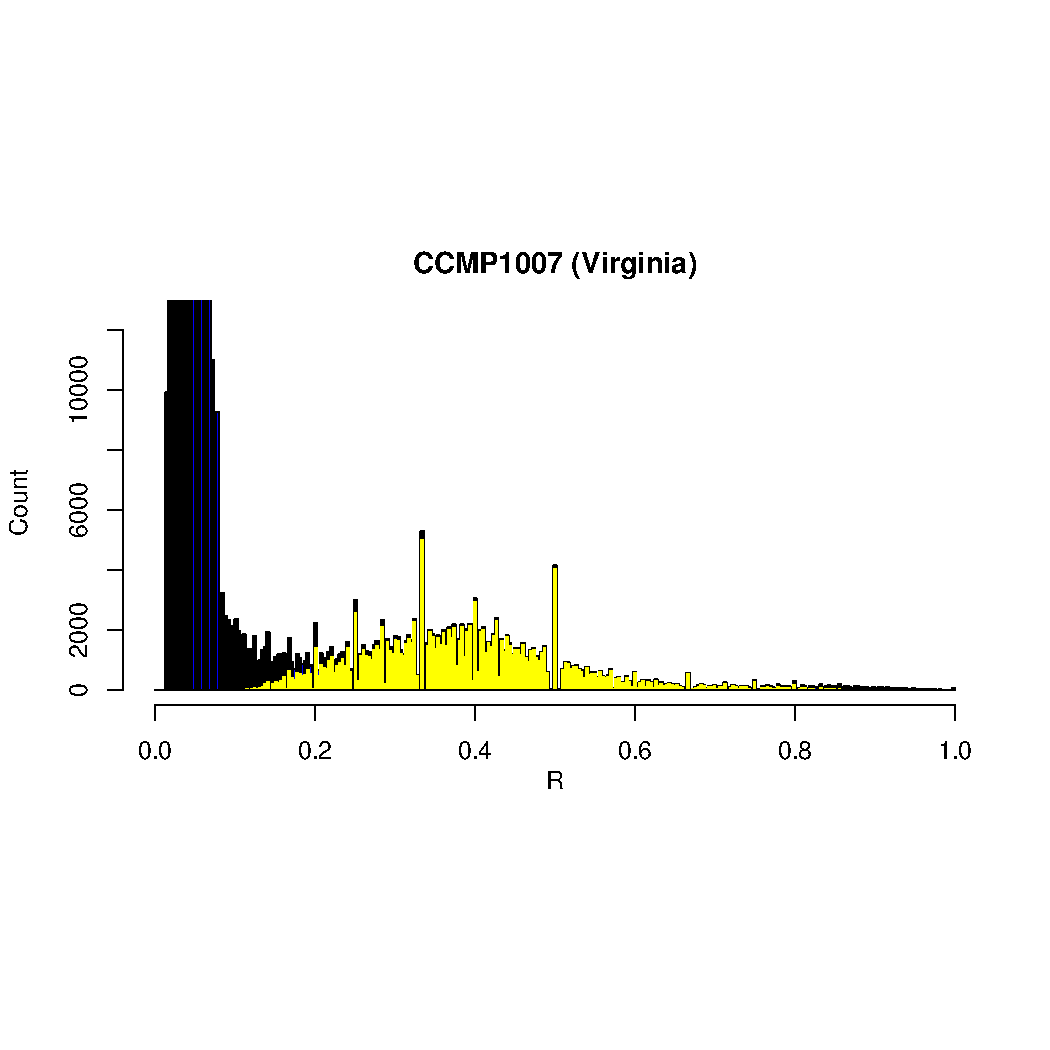
\includegraphics[width=\maxwidth]{FigS7-hwe-histo-figs-knitr/unnamed-chunk-10-1} 
\begin{kframe}\begin{verbatim}
#      [,1]     [,2]     [,3]   [,4]    [,5]  [,6]    [,7]    [,8]     [,9]     [,10]    [,11] 
# [1,] "blue"   "nm3"    "nm3x" "nm3hi" "red" "black" "green" "orange" "ornghi" "nzgrey" "grey"
# [2,] "201775" "189058" NA     "0"     NA    NA      NA      NA       NA       NA       NA
# 
# homnr:het ratios vs mod.humpth lo x hi, full-unfiltered :
#       hi
# lo          0.7     0.75     0.76     0.77     0.78     0.79      0.8     0.85      0.9
#   0.1  24.88452 33.21615 34.06024 36.83314 39.20644 42.54507 47.51026 77.67108 182.8116
#   0.15 22.01175 29.41870 30.16911 32.63426 34.74416 37.71226 42.12639 68.93983 162.4114
#   0.16 21.56408 28.82694 29.56275 31.97994 34.04879 36.95915 41.28741 67.57922 159.2324
#   0.17 21.21341 28.36340 29.08777 31.46740 33.50410 36.36923 40.63023 66.51344 156.7423
#   0.18 20.81365 27.83496 28.54630 30.88310 32.88315 35.69671 39.88103 65.29844 153.9035
#   0.19 20.44952 27.35363 28.05309 30.35089 32.31755 35.08415 39.19861 64.19174 151.3177
#   0.2  19.87647 26.59613 27.27690 29.51331 31.42743 34.12012 38.12466 62.45006 147.2484
#   0.25 17.59483 23.58008 24.18645 26.17843 27.88335 30.28175 33.84863 55.51544 131.0459
# 
# 
# 1012 coverage summary for retained sites:
#    Min. 1st Qu.  Median    Mean 3rd Qu.    Max. 
#   29.00   53.00   66.00   67.35   81.00  113.00 
# FigS7-hwe-histo-figs-mine/S7-full-unfiltered-1012chronly.pdf :
#   based on 28631165 positions with coverage in [ 28.02323 , 113.5889 ]
\end{verbatim}
\end{kframe}
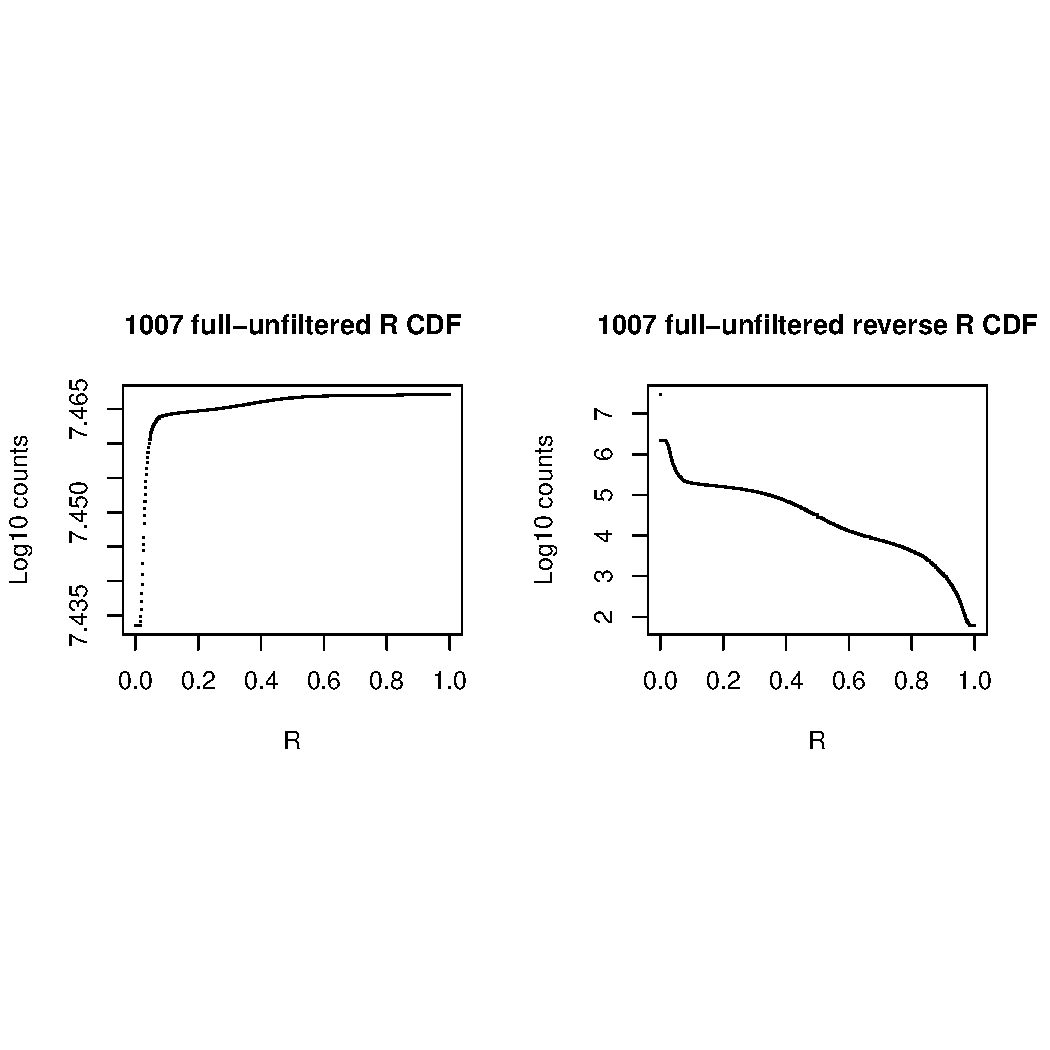
\includegraphics[width=\maxwidth]{FigS7-hwe-histo-figs-knitr/unnamed-chunk-10-2} 
\begin{kframe}\begin{verbatim}
#      [,1]     [,2]     [,3]     [,4]    [,5]  [,6]    [,7]    [,8]     [,9]     [,10]    [,11] 
# [1,] "blue"   "nm3"    "nm3x"   "nm3hi" "red" "black" "green" "orange" "ornghi" "nzgrey" "grey"
# [2,] "229627" "157109" "314218" "5677"  NA    NA      NA      "314218" "5677"   NA       NA    
# FigS7-hwe-histo-figs-mine/S7-full-unfiltered-1012chronly.pdf written; 301-bin histo follows:
\end{verbatim}
\end{kframe}
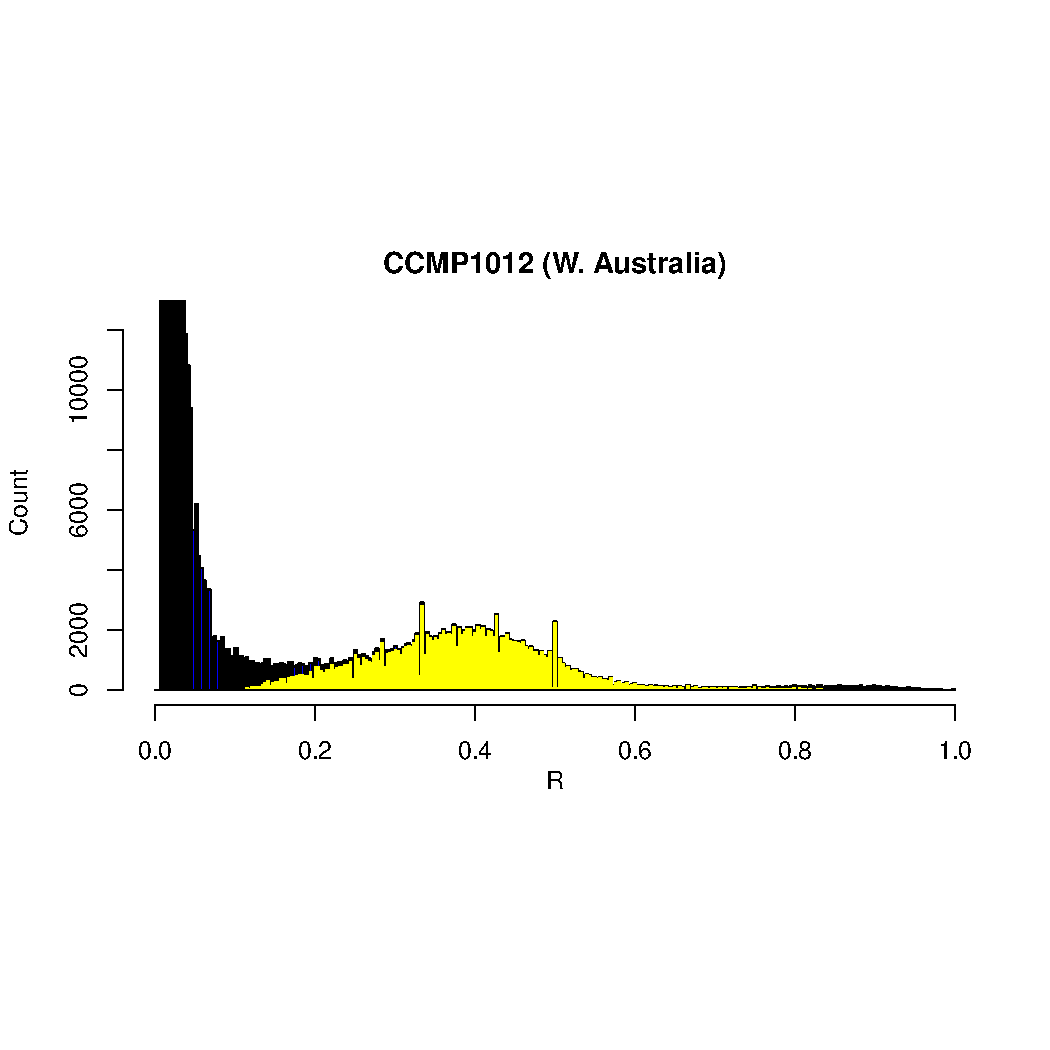
\includegraphics[width=\maxwidth]{FigS7-hwe-histo-figs-knitr/unnamed-chunk-10-3} 
\begin{kframe}\begin{verbatim}
#      [,1]     [,2]     [,3]   [,4]    [,5]  [,6]    [,7]    [,8]     [,9]     [,10]    [,11] 
# [1,] "blue"   "nm3"    "nm3x" "nm3hi" "red" "black" "green" "orange" "ornghi" "nzgrey" "grey"
# [2,] "229627" "218960" NA     "0"     NA    NA      NA      NA       NA       NA       NA
# 
# homnr:het ratios vs mod.humpth lo x hi, full-unfiltered :
#       hi
# lo          0.7     0.75     0.76     0.77     0.78     0.79      0.8     0.85       0.9
#   0.1  23.46121 27.96229 28.84008 30.03588 31.47903 33.08175 35.71851 54.10509 115.34067
#   0.15 21.57790 25.73244 26.54264 27.64638 28.97842 30.45774 32.89149 49.86246 106.38341
#   0.16 21.25281 25.34752 26.14606 27.23390 28.54676 30.00479 32.40349 49.13010 104.83721
#   0.17 20.94198 24.97950 25.76689 26.83954 28.13406 29.57172 31.93692 48.42989 103.35889
#   0.18 20.59535 24.56908 25.34403 26.39973 27.67380 29.08875 31.41658 47.64900 101.71025
#   0.19 20.28096 24.19684 24.96050 26.00084 27.25636 28.65071 30.94465 46.94076 100.21496
#   0.2  19.88397 23.72680 24.47622 25.49715 26.72925 28.09759 30.34874 46.04644  98.32684
#   0.25 18.04982 21.55516 22.23876 23.17002 24.29391 25.54207 27.59552 41.91456  89.60339
# 
# 
# 1013 coverage summary for retained sites:
#    Min. 1st Qu.  Median    Mean 3rd Qu.    Max. 
#   26.00   51.00   63.00   64.81   77.00  113.00 
# FigS7-hwe-histo-figs-mine/S7-full-unfiltered-1013chronly.pdf :
#   based on 28362674 positions with coverage in [ 25.47672 , 113.8454 ]
\end{verbatim}
\end{kframe}
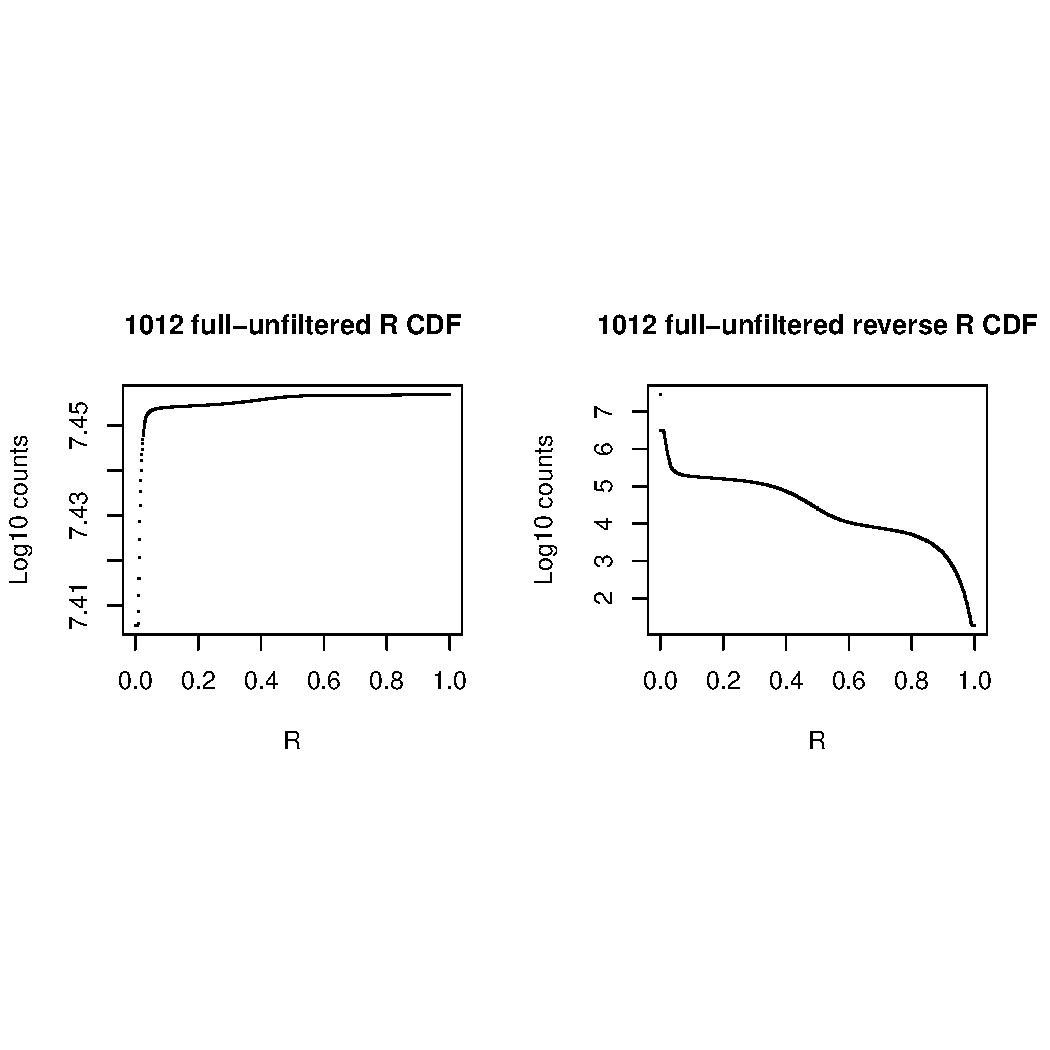
\includegraphics[width=\maxwidth]{FigS7-hwe-histo-figs-knitr/unnamed-chunk-10-4} 
\begin{kframe}\begin{verbatim}
#      [,1]     [,2]     [,3]     [,4]    [,5]  [,6]    [,7]    [,8]     [,9]     [,10]    [,11] 
# [1,] "blue"   "nm3"    "nm3x"   "nm3hi" "red" "black" "green" "orange" "ornghi" "nzgrey" "grey"
# [2,] "390935" "238281" "476562" "48719" NA    NA      NA      "476562" "48719"  NA       NA    
# FigS7-hwe-histo-figs-mine/S7-full-unfiltered-1013chronly.pdf written; 301-bin histo follows:
\end{verbatim}
\end{kframe}
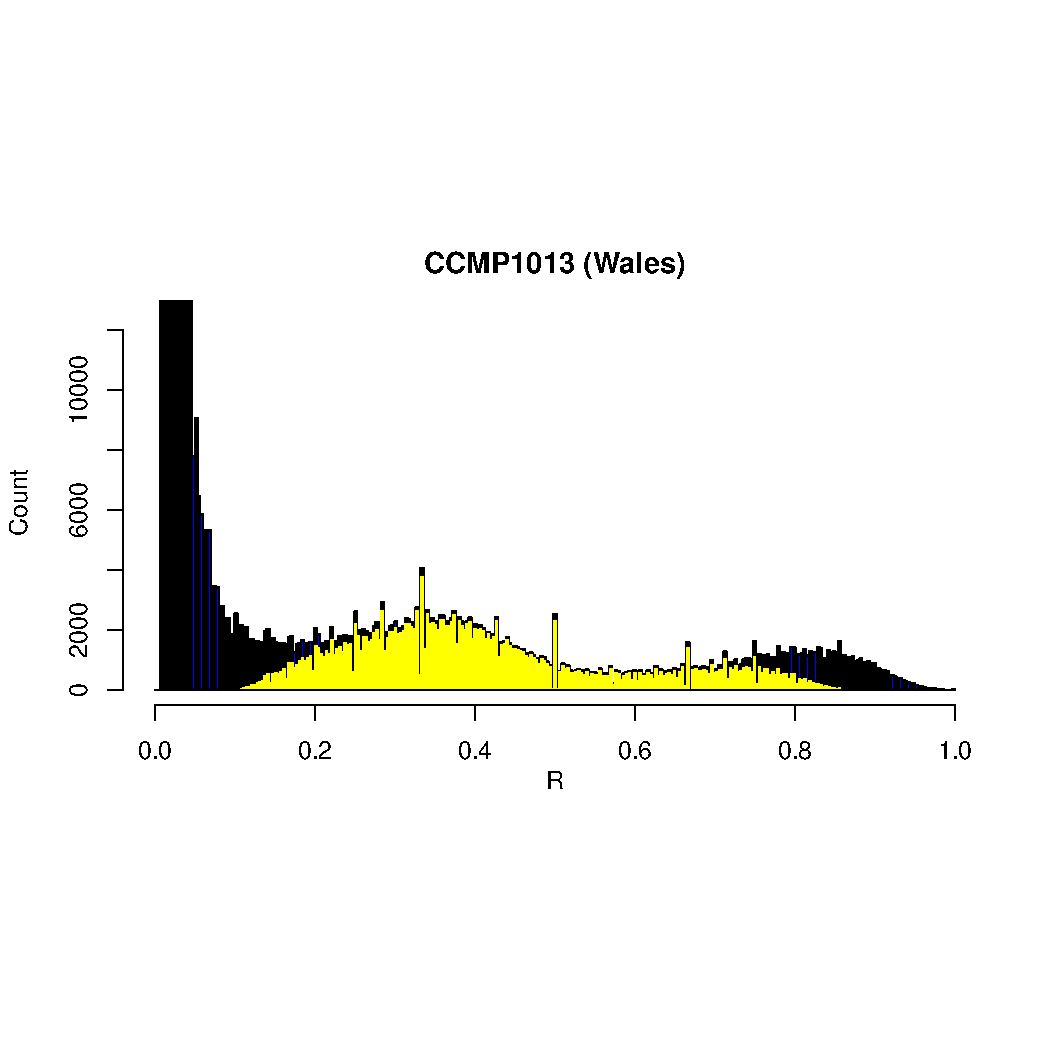
\includegraphics[width=\maxwidth]{FigS7-hwe-histo-figs-knitr/unnamed-chunk-10-5} 
\begin{kframe}\begin{verbatim}
#      [,1]     [,2]     [,3]   [,4]    [,5]  [,6]    [,7]    [,8]     [,9]     [,10]    [,11] 
# [1,] "blue"   "nm3"    "nm3x" "nm3hi" "red" "black" "green" "orange" "ornghi" "nzgrey" "grey"
# [2,] "390935" "299573" NA     "0"     NA    NA      NA      NA       NA       NA       NA
# 
# homnr:het ratios vs mod.humpth lo x hi, full-unfiltered :
#       hi
# lo          0.7     0.75     0.76     0.77     0.78     0.79      0.8      0.85      0.9
#   0.1  3.543958 4.642082 4.893028 5.245136 5.688758 6.186528 6.910646 13.113563 41.85776
#   0.15 3.175237 4.184254 4.414837 4.738373 5.145997 5.603376 6.268735 11.968314 38.38005
#   0.16 3.112576 4.106450 4.333572 4.652253 5.053759 5.504274 6.159648 11.773689 37.78905
#   0.17 3.054242 4.034019 4.257919 4.572080 4.967891 5.412015 6.058093 11.592504 37.23885
#   0.18 2.987545 3.951203 4.171420 4.480413 4.869712 5.306530 5.941979 11.385342 36.60978
#   0.19 2.926322 3.875185 4.092021 4.396269 4.779591 5.209702 5.835395 11.195183 36.03233
#   0.2  2.847336 3.777110 3.989584 4.287712 4.663323 5.084782 5.697887 10.949852 35.28735
#   0.25 2.495148 3.339810 3.532834 3.803670 4.144898 4.527776 5.084757  9.855953 31.96558
# 
# 
# 1014 coverage summary for retained sites:
#    Min. 1st Qu.  Median    Mean 3rd Qu.    Max. 
#   14.00   24.00   30.00   31.03   37.00   52.00 
# FigS7-hwe-histo-figs-mine/S7-full-unfiltered-1014chronly.pdf :
#   based on 28207955 positions with coverage in [ 13.94298 , 52.25889 ]
\end{verbatim}
\end{kframe}
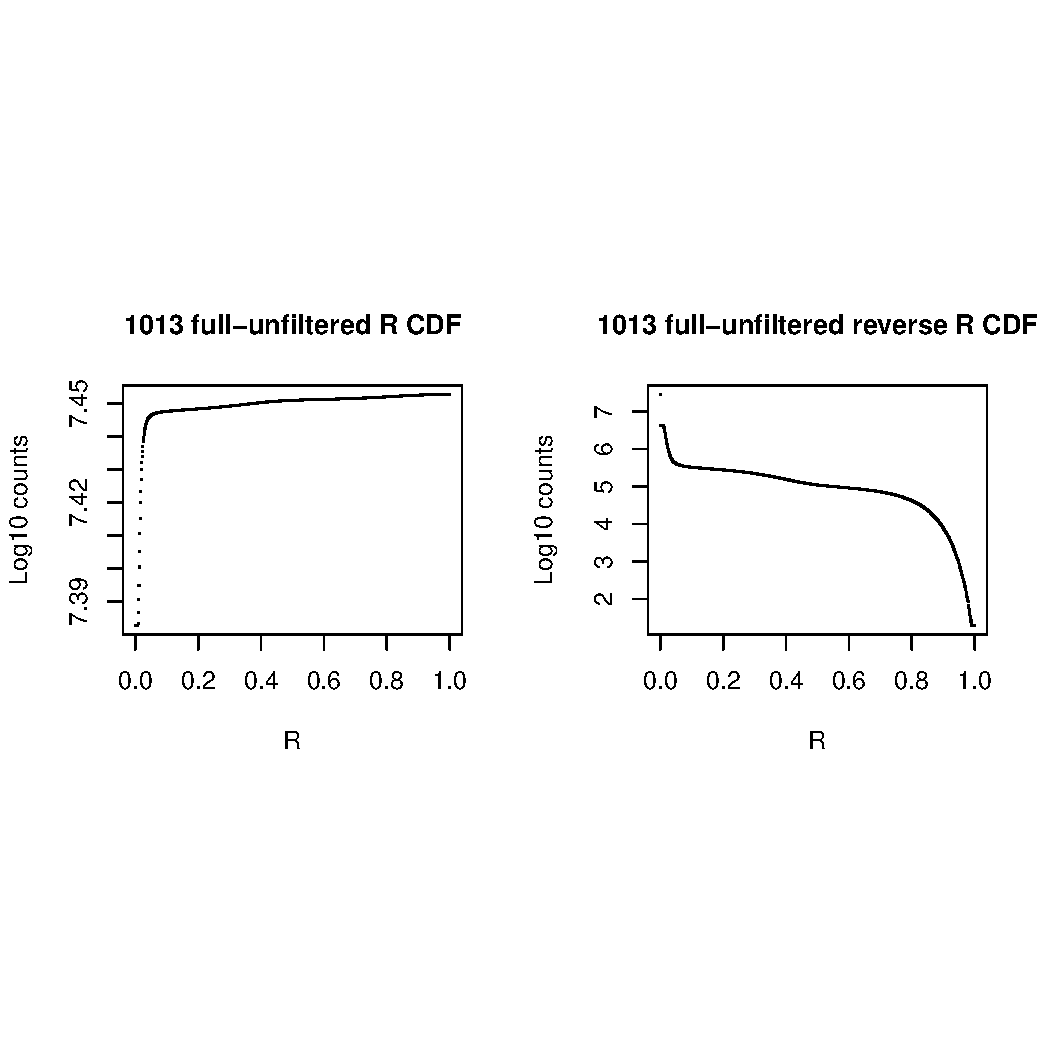
\includegraphics[width=\maxwidth]{FigS7-hwe-histo-figs-knitr/unnamed-chunk-10-6} 
\begin{kframe}\begin{verbatim}
#      [,1]     [,2]    [,3]     [,4]    [,5]  [,6]    [,7]    [,8]     [,9]     [,10]    [,11] 
# [1,] "blue"   "nm3"   "nm3x"   "nm3hi" "red" "black" "green" "orange" "ornghi" "nzgrey" "grey"
# [2,] "147635" "79824" "159648" "33"    NA    NA      NA      "159648" "33"     NA       NA    
# FigS7-hwe-histo-figs-mine/S7-full-unfiltered-1014chronly.pdf written; 301-bin histo follows:
\end{verbatim}
\end{kframe}
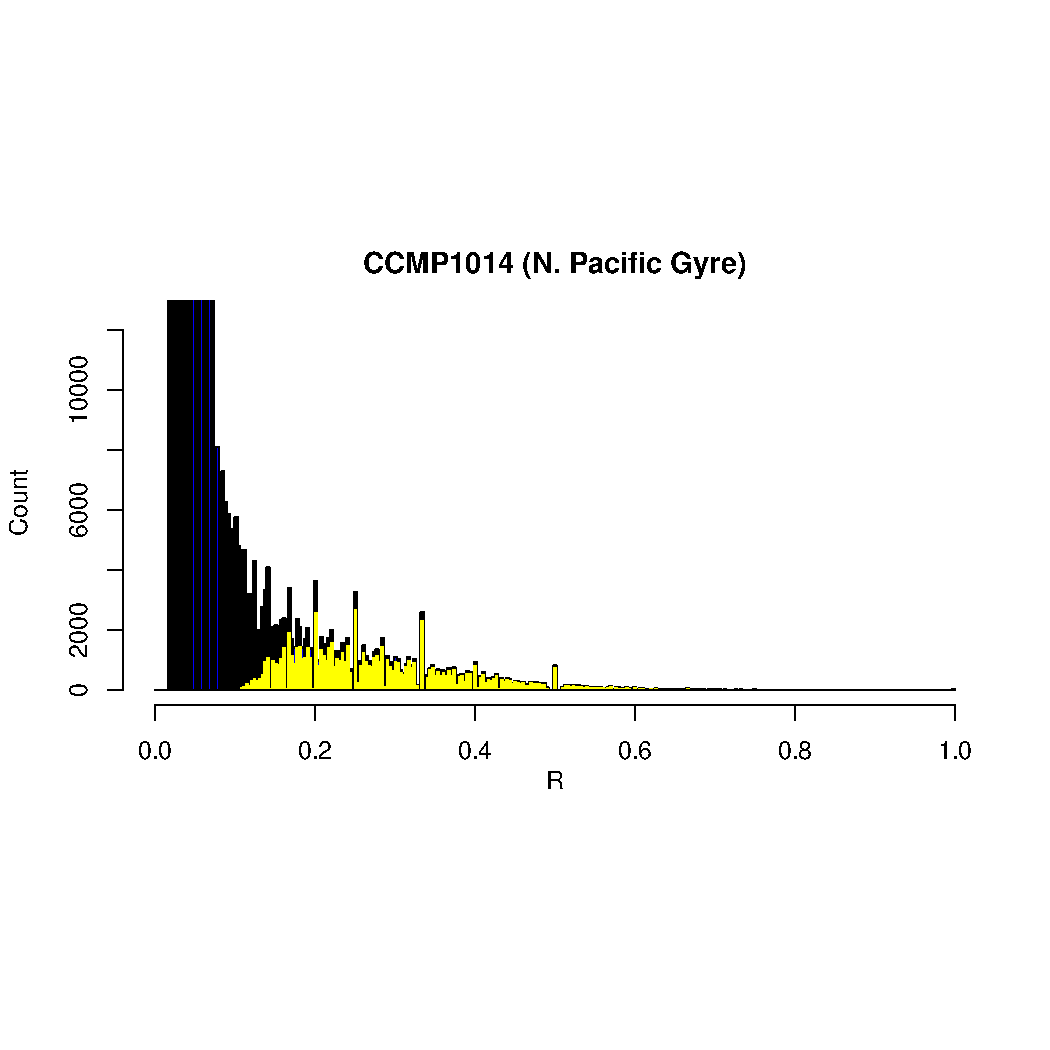
\includegraphics[width=\maxwidth]{FigS7-hwe-histo-figs-knitr/unnamed-chunk-10-7} 
\begin{kframe}\begin{verbatim}
#      [,1]     [,2]     [,3]   [,4]    [,5]  [,6]    [,7]    [,8]     [,9]     [,10]    [,11] 
# [1,] "blue"   "nm3"    "nm3x" "nm3hi" "red" "black" "green" "orange" "ornghi" "nzgrey" "grey"
# [2,] "147635" "146828" NA     "0"     NA    NA      NA      NA       NA       NA       NA
# 
# homnr:het ratios vs mod.humpth lo x hi, full-unfiltered :
#       hi
# lo           0.7    0.75     0.76     0.77     0.78     0.79      0.8      0.85       0.9
#   0.1  1051.2517 3092.62 3290.085 3866.025 4686.303 5155.033 6724.261 11897.538 11897.538
#   0.15  675.1633 1986.92 2113.809 2483.900 3011.000 3312.200 4320.565  7644.846  7644.846
#   0.16  632.9388 1862.78 1981.745 2328.725 2822.909 3105.300 4050.696  7167.385  7167.385
#   0.17  598.5102 1761.56 1874.064 2202.200 2669.545 2936.600 3830.652  6778.077  6778.077
#   0.18  556.4830 1638.00 1742.617 2047.750 2482.333 2730.667 3562.043  6302.846  6302.846
#   0.19  522.4082 1537.82 1636.043 1922.525 2330.545 2563.700 3344.261  5917.538  5917.538
#   0.2   472.2245 1390.28 1479.085 1738.100 2107.000 2317.800 3023.522  5350.077  5350.077
#   0.25  325.3197  958.38 1019.617 1198.225 1452.606 1597.967 2084.609  3688.923  3688.923
# 
# 
# 1015 coverage summary for retained sites:
#    Min. 1st Qu.  Median    Mean 3rd Qu.    Max. 
#   26.00   47.00   57.00   58.47   69.00   97.00 
# FigS7-hwe-histo-figs-mine/S7-full-unfiltered-1015chronly.pdf :
#   based on 28534472 positions with coverage in [ 25.72318 , 97.34986 ]
\end{verbatim}
\end{kframe}
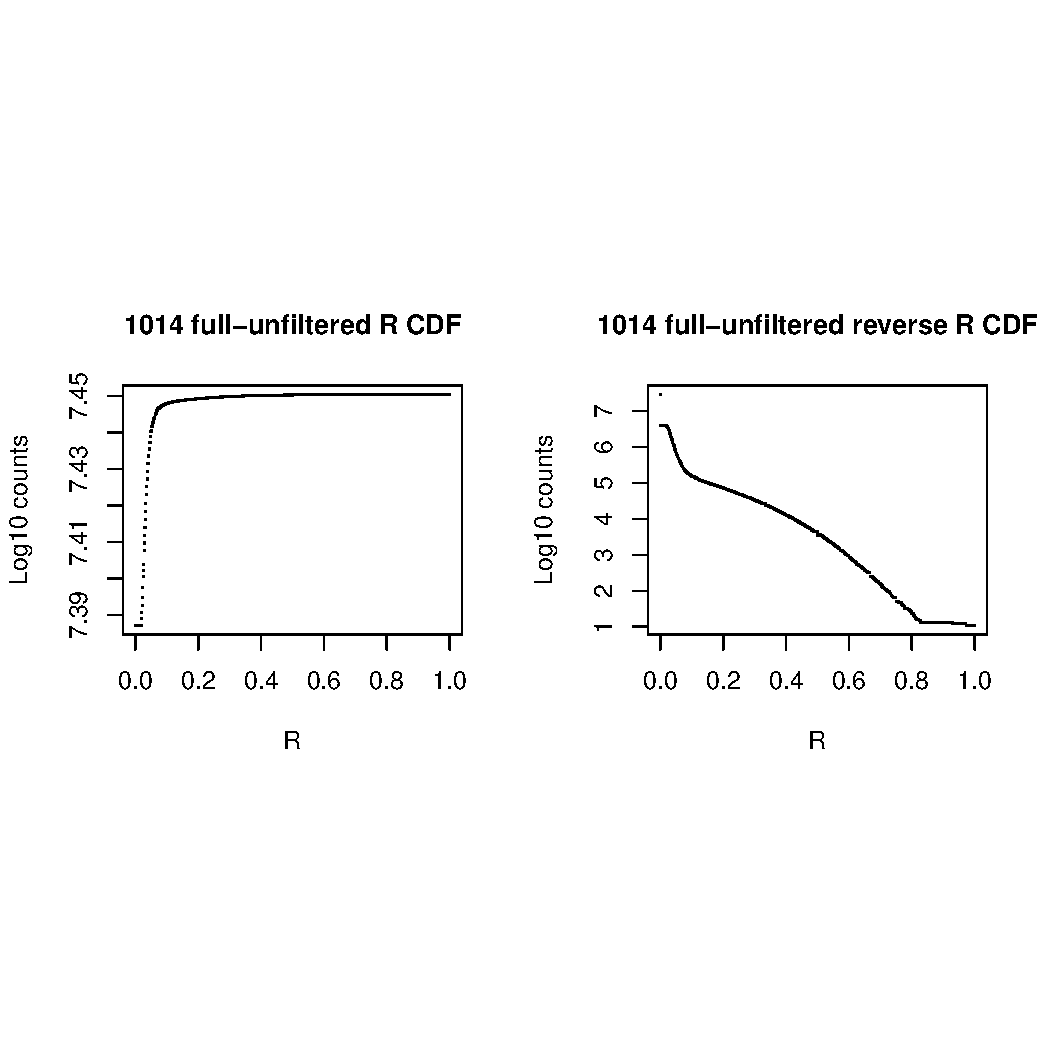
\includegraphics[width=\maxwidth]{FigS7-hwe-histo-figs-knitr/unnamed-chunk-10-8} 
\begin{kframe}\begin{verbatim}
#      [,1]     [,2]     [,3]     [,4]    [,5]  [,6]    [,7]    [,8]     [,9]     [,10]    [,11] 
# [1,] "blue"   "nm3"    "nm3x"   "nm3hi" "red" "black" "green" "orange" "ornghi" "nzgrey" "grey"
# [2,] "228154" "167786" "335572" "2426"  NA    NA      NA      "335572" "2426"   NA       NA    
# FigS7-hwe-histo-figs-mine/S7-full-unfiltered-1015chronly.pdf written; 301-bin histo follows:
\end{verbatim}
\end{kframe}
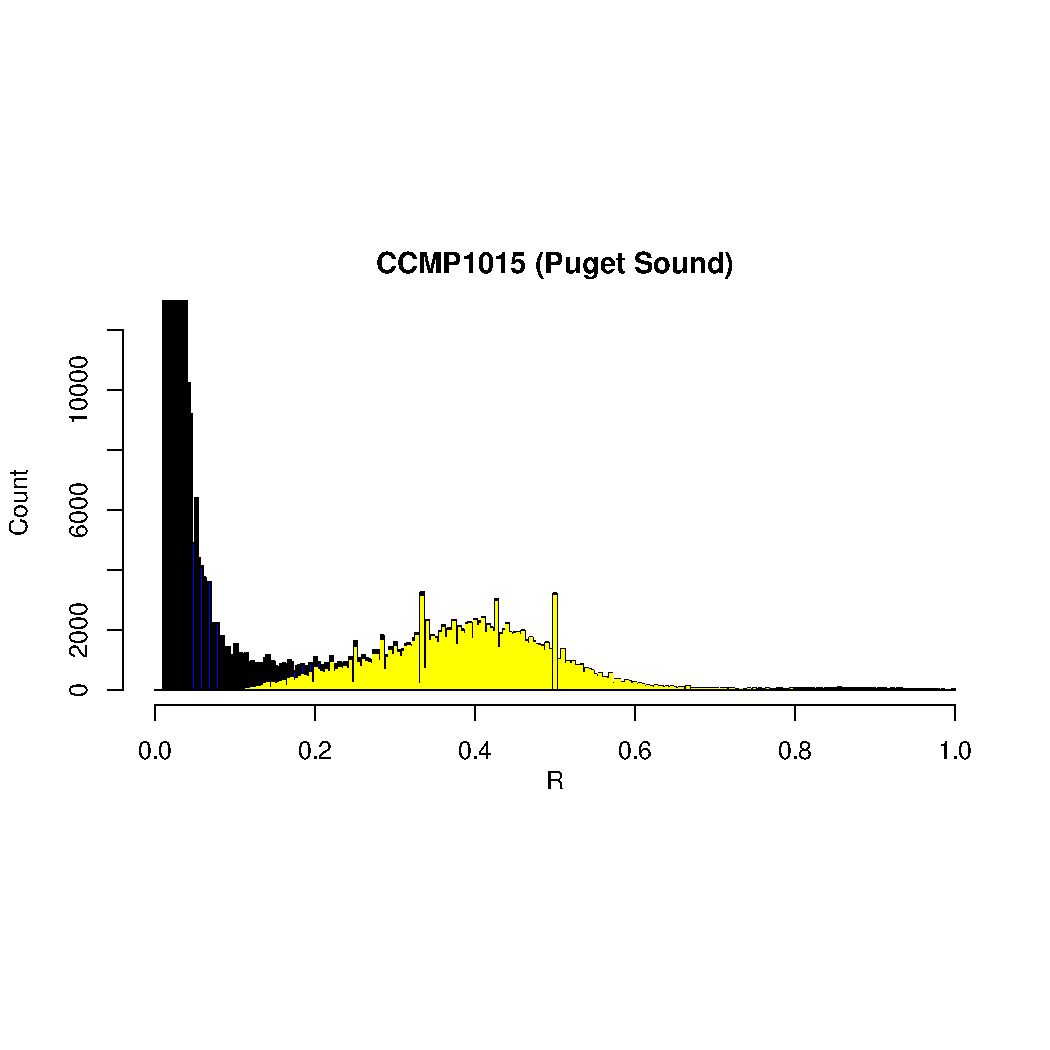
\includegraphics[width=\maxwidth]{FigS7-hwe-histo-figs-knitr/unnamed-chunk-10-9} 
\begin{kframe}\begin{verbatim}
#      [,1]     [,2]     [,3]   [,4]    [,5]  [,6]    [,7]    [,8]     [,9]     [,10]    [,11] 
# [1,] "blue"   "nm3"    "nm3x" "nm3hi" "red" "black" "green" "orange" "ornghi" "nzgrey" "grey"
# [2,] "228154" "221948" NA     "0"     NA    NA      NA      NA       NA       NA       NA
# 
# homnr:het ratios vs mod.humpth lo x hi, full-unfiltered :
#       hi
# lo          0.7     0.75     0.76     0.77     0.78     0.79      0.8      0.85      0.9
#   0.1  57.11623 69.31111 71.31323 74.48064 78.29499 81.97678 87.57458 125.39424 258.7631
#   0.15 52.61186 63.86157 65.70851 68.63043 72.14914 75.54557 80.70950 115.59790 238.6299
#   0.16 51.90033 63.00073 64.82315 67.70630 71.17831 74.52966 79.62506 114.05043 235.4495
#   0.17 51.21229 62.16831 63.96703 66.81267 70.23952 73.54729 78.57641 112.55403 232.3742
#   0.18 50.45077 61.24699 63.01948 65.82362 69.20049 72.46002 77.41579 110.89784 228.9704
#   0.19 49.74977 60.39891 62.14725 64.91318 68.24404 71.45916 76.34741 109.37328 225.8371
#   0.2  48.85005 59.31038 61.02773 63.74462 67.01643 70.17455 74.97614 107.41650 221.8156
#   0.25 44.71876 54.31220 55.88722 58.37896 61.37962 64.27601 68.67967  98.43157 203.3499
# 
# 
# 3367 coverage summary for retained sites:
#    Min. 1st Qu.  Median    Mean 3rd Qu.    Max. 
#   29.00   52.00   62.00   62.43   73.00   99.00 
# FigS7-hwe-histo-figs-mine/S7-full-unfiltered-3367chronly.pdf :
#   based on 28736089 positions with coverage in [ 28.82008 , 99.23682 ]
\end{verbatim}
\end{kframe}
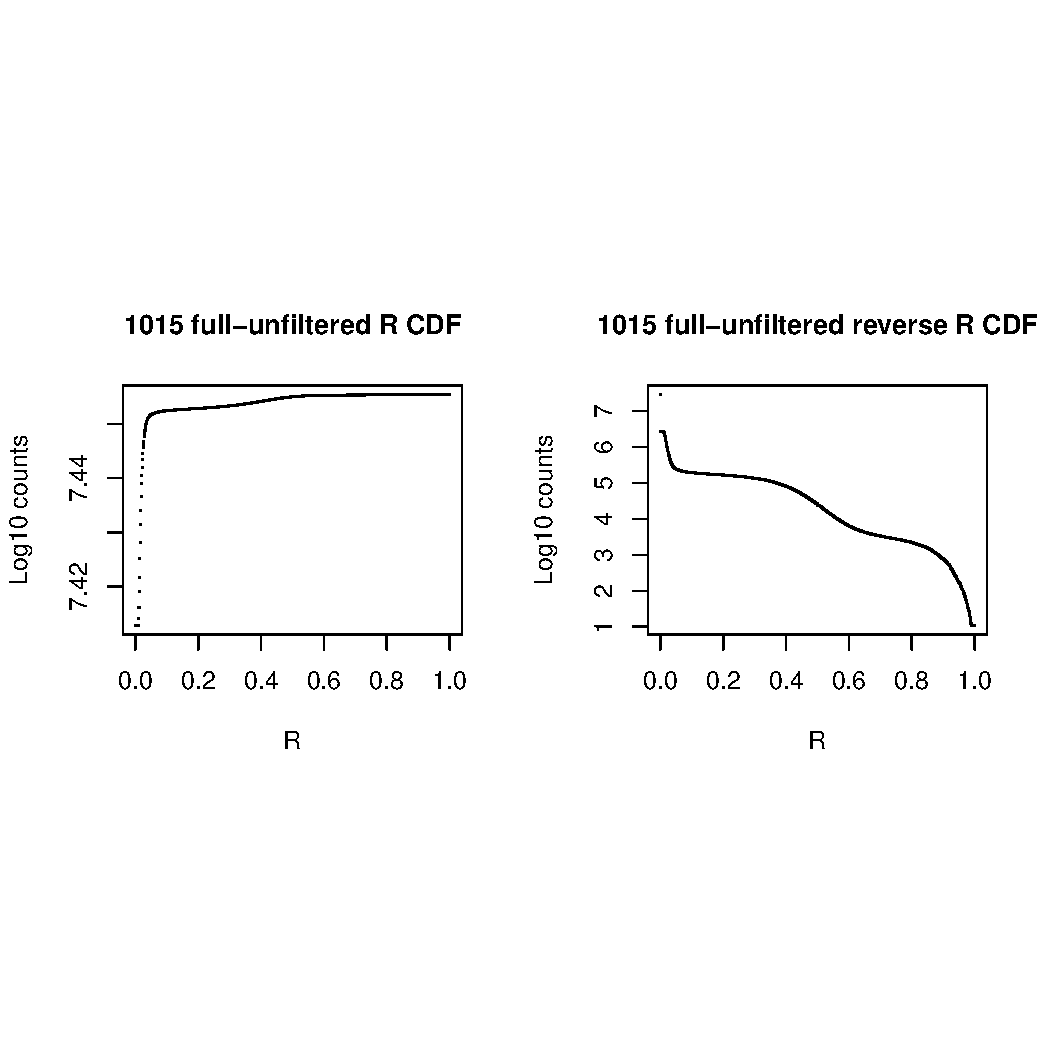
\includegraphics[width=\maxwidth]{FigS7-hwe-histo-figs-knitr/unnamed-chunk-10-10} 
\begin{kframe}\begin{verbatim}
#      [,1]     [,2]     [,3]     [,4]    [,5]  [,6]    [,7]    [,8]     [,9]     [,10]    [,11] 
# [1,] "blue"   "nm3"    "nm3x"   "nm3hi" "red" "black" "green" "orange" "ornghi" "nzgrey" "grey"
# [2,] "361564" "216091" "432182" "56690" NA    NA      NA      "432182" "56690"  NA       NA    
# FigS7-hwe-histo-figs-mine/S7-full-unfiltered-3367chronly.pdf written; 301-bin histo follows:
\end{verbatim}
\end{kframe}
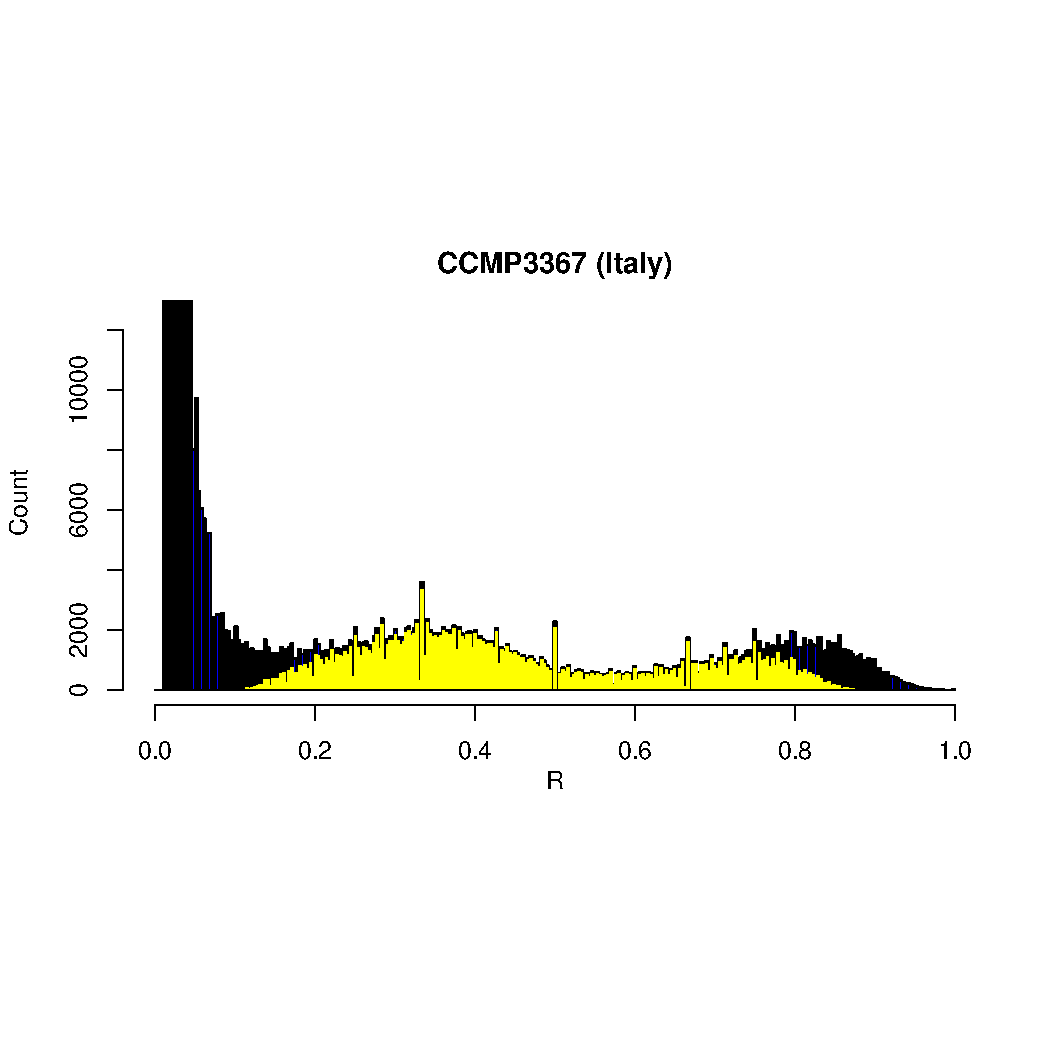
\includegraphics[width=\maxwidth]{FigS7-hwe-histo-figs-knitr/unnamed-chunk-10-11} 
\begin{kframe}\begin{verbatim}
#      [,1]     [,2]     [,3]   [,4]    [,5]  [,6]    [,7]    [,8]     [,9]     [,10]    [,11] 
# [1,] "blue"   "nm3"    "nm3x" "nm3hi" "red" "black" "green" "orange" "ornghi" "nzgrey" "grey"
# [2,] "361564" "254309" NA     "0"     NA    NA      NA      NA       NA       NA       NA
# 
# homnr:het ratios vs mod.humpth lo x hi, full-unfiltered :
#       hi
# lo          0.7     0.75     0.76     0.77     0.78     0.79      0.8      0.85      0.9
#   0.1  2.543089 3.441612 3.666529 3.962187 4.353404 4.797482 5.485629 11.399230 43.36521
#   0.15 2.301579 3.138856 3.348443 3.623947 3.988497 4.402306 5.043547 10.554055 40.34112
#   0.16 2.259910 3.086620 3.293561 3.565589 3.925538 4.334123 4.967271 10.408232 39.81936
#   0.17 2.219632 3.036127 3.240511 3.509177 3.864679 4.268216 4.893541 10.267275 39.31500
#   0.18 2.174058 2.978995 3.180486 3.445350 3.795819 4.193644 4.810118 10.107786 38.74434
#   0.19 2.132284 2.926628 3.125467 3.386845 3.732702 4.125292 4.733652  9.961598 38.22127
#   0.2  2.080464 2.861667 3.057217 3.314270 3.654405 4.040500 4.638795  9.780251 37.57240
#   0.25 1.840126 2.560378 2.740671 2.977669 3.291267 3.647238 4.198855  8.939173 34.56297
# 
# 
# 1335 coverage summary for retained sites:
#    Min. 1st Qu.  Median    Mean 3rd Qu.    Max. 
#    56.0    88.0   106.0   105.6   123.0   159.0 
# FigS7-hwe-histo-figs-mine/S7-full-unfiltered-1335chronly.pdf :
#   based on 27041564 positions with coverage in [ 55.82708 , 159.6581 ]
\end{verbatim}
\end{kframe}
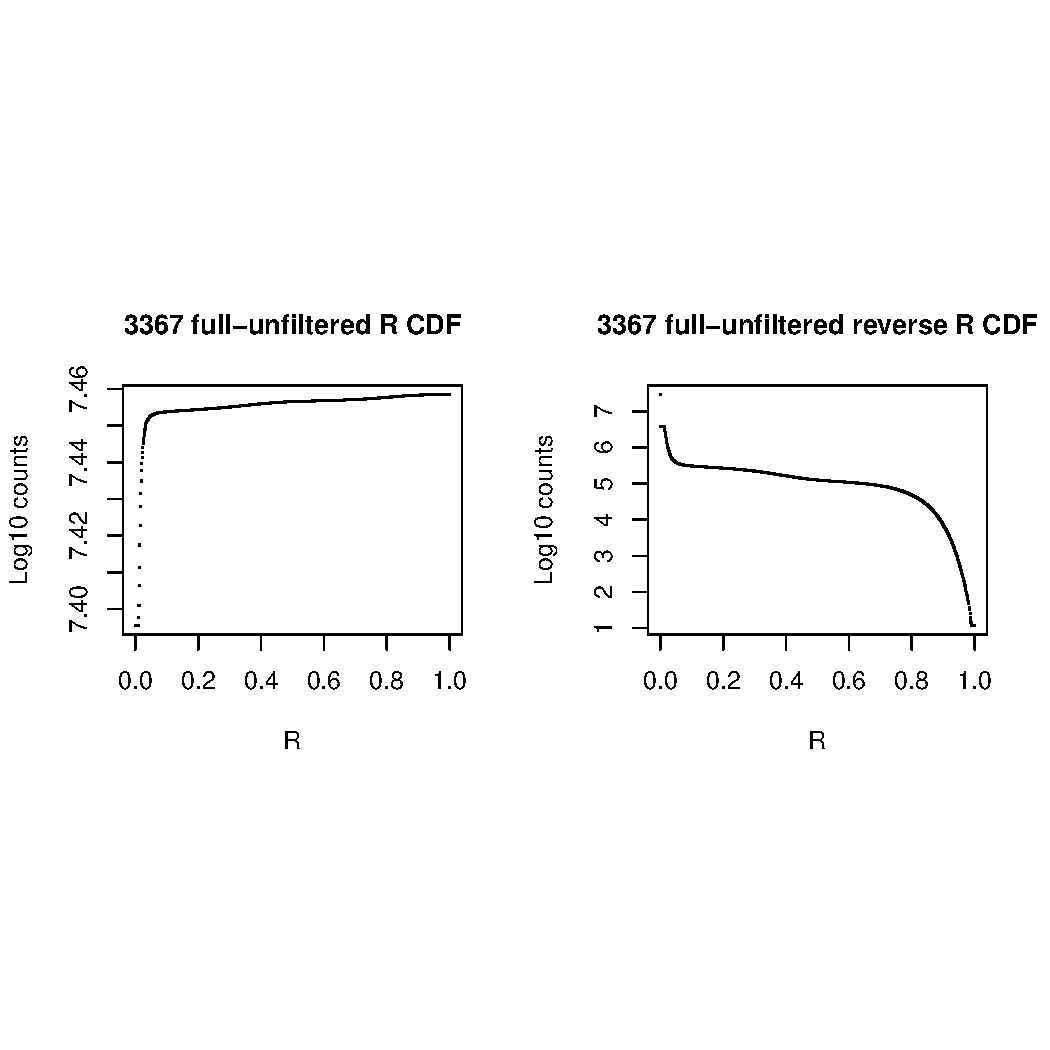
\includegraphics[width=\maxwidth]{FigS7-hwe-histo-figs-knitr/unnamed-chunk-10-12} 
\begin{kframe}\begin{verbatim}
#      [,1]     [,2]     [,3]     [,4]    [,5]  [,6]    [,7]    [,8]     [,9]     [,10]    [,11] 
# [1,] "blue"   "nm3"    "nm3x"   "nm3hi" "red" "black" "green" "orange" "ornghi" "nzgrey" "grey"
# [2,] "292931" "137007" "274014" "86"    NA    NA      NA      "274014" "86"     NA       NA    
# FigS7-hwe-histo-figs-mine/S7-full-unfiltered-1335chronly.pdf written; 301-bin histo follows:
\end{verbatim}
\end{kframe}
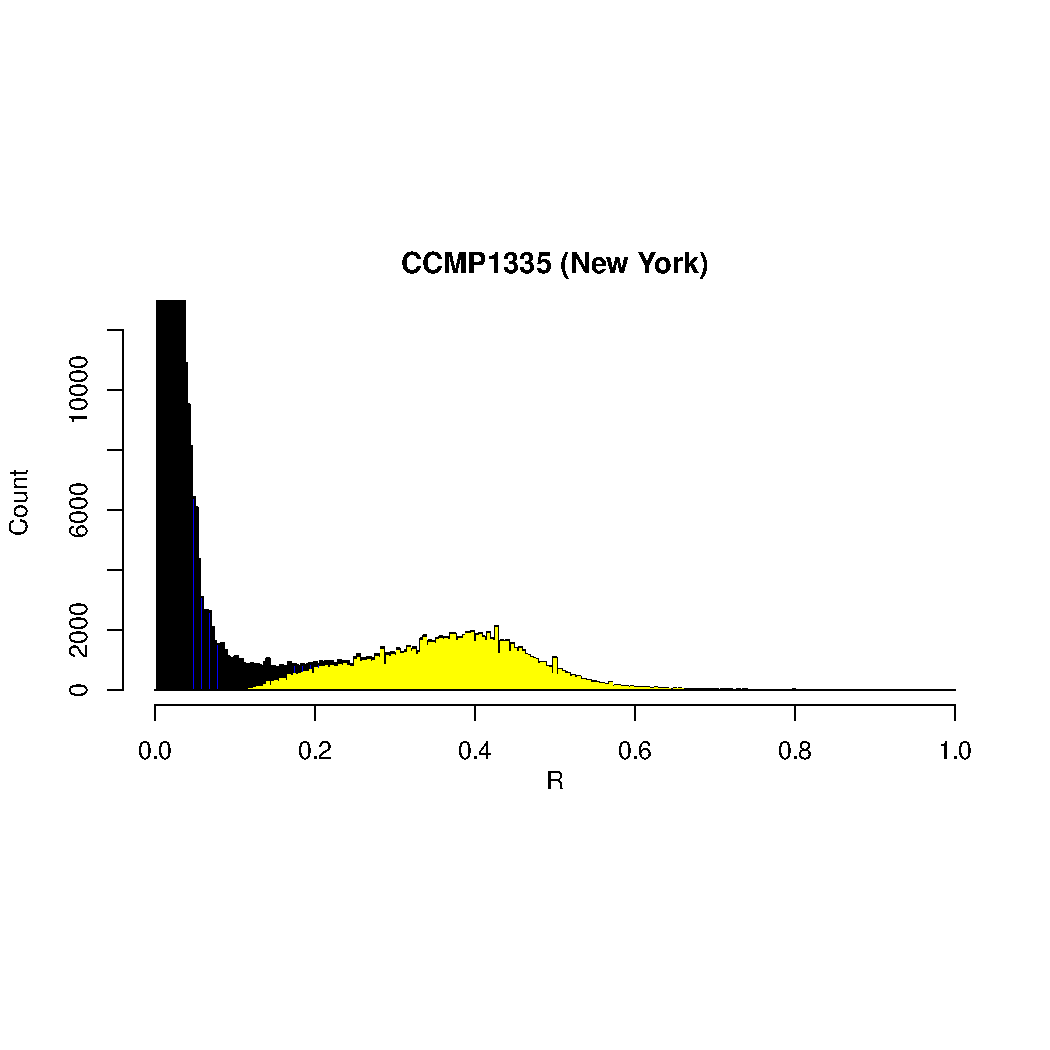
\includegraphics[width=\maxwidth]{FigS7-hwe-histo-figs-knitr/unnamed-chunk-10-13} 
\begin{kframe}\begin{verbatim}
#      [,1]     [,2]     [,3]   [,4]    [,5]  [,6]    [,7]    [,8]     [,9]     [,10]    [,11] 
# [1,] "blue"   "nm3"    "nm3x" "nm3hi" "red" "black" "green" "orange" "ornghi" "nzgrey" "grey"
# [2,] "292931" "291331" NA     "0"     NA    NA      NA      NA       NA       NA       NA
# 
# homnr:het ratios vs mod.humpth lo x hi, full-unfiltered :
#       hi
# lo          0.7      0.75     0.76    0.77     0.78     0.79      0.8     0.85      0.9
#   0.1  608.8269 1247.4646 1365.853 1584.55 1842.663 2113.067 2476.422 5466.414 14413.09
#   0.15 555.7615 1138.8268 1246.914 1446.58 1682.233 1929.107 2260.844 4990.655 13158.82
#   0.16 546.9154 1120.7165 1227.086 1423.58 1655.488 1898.440 2224.906 4911.345 12949.73
#   0.17 537.7769 1102.0079 1206.603 1399.82 1627.860 1866.760 2187.781 4829.414 12733.73
#   0.18 528.1654 1082.3307 1185.060 1374.83 1598.802 1833.440 2148.734 4743.241 12506.55
#   0.19 518.4192 1062.3780 1163.216 1349.49 1569.337 1799.653 2109.141 4655.862 12276.18
#   0.2  507.6346 1040.2992 1139.043 1321.45 1536.733 1762.267 2065.328 4559.172 12021.27
#   0.25 453.3462  929.1575 1017.362 1180.30 1372.605 1574.067 1844.781 4072.448 10738.09
# 
# 
# 
# ***
# *
# * Processing Chr1-unfiltered 
# *
# ***
# Chr1-unfiltered coverage stats:
#                   1007     1012     1013     1014     1015     3367      1335
# cov.means.all 36.28163 68.20058 66.69089 31.26632 59.47042 62.38345 103.91248
# cov.sigs.all  12.74224 23.95397 28.53029 11.58852 21.20817 21.64174  32.96697
# cov.means     36.28163 68.20058 66.69089 31.26632 59.47042 62.38345 103.91248
# cov.sigs      12.74224 23.95397 28.53029 11.58852 21.20817 21.64174  32.96697
# cov.min       23.53939 44.24661 38.16060 19.67780 38.26224 40.74172  70.94551
# 
# 
# 1007 coverage summary for retained sites:
#    Min. 1st Qu.  Median    Mean 3rd Qu.    Max. 
#   24.00   30.00   35.00   35.43   41.00   49.00 
# FigS7-hwe-histo-figs-mine/S7-Chr1-unfiltered-1007.pdf :
#   based on 2345963 positions with coverage in [ 23.53939 , 49.02388 ]
\end{verbatim}
\end{kframe}
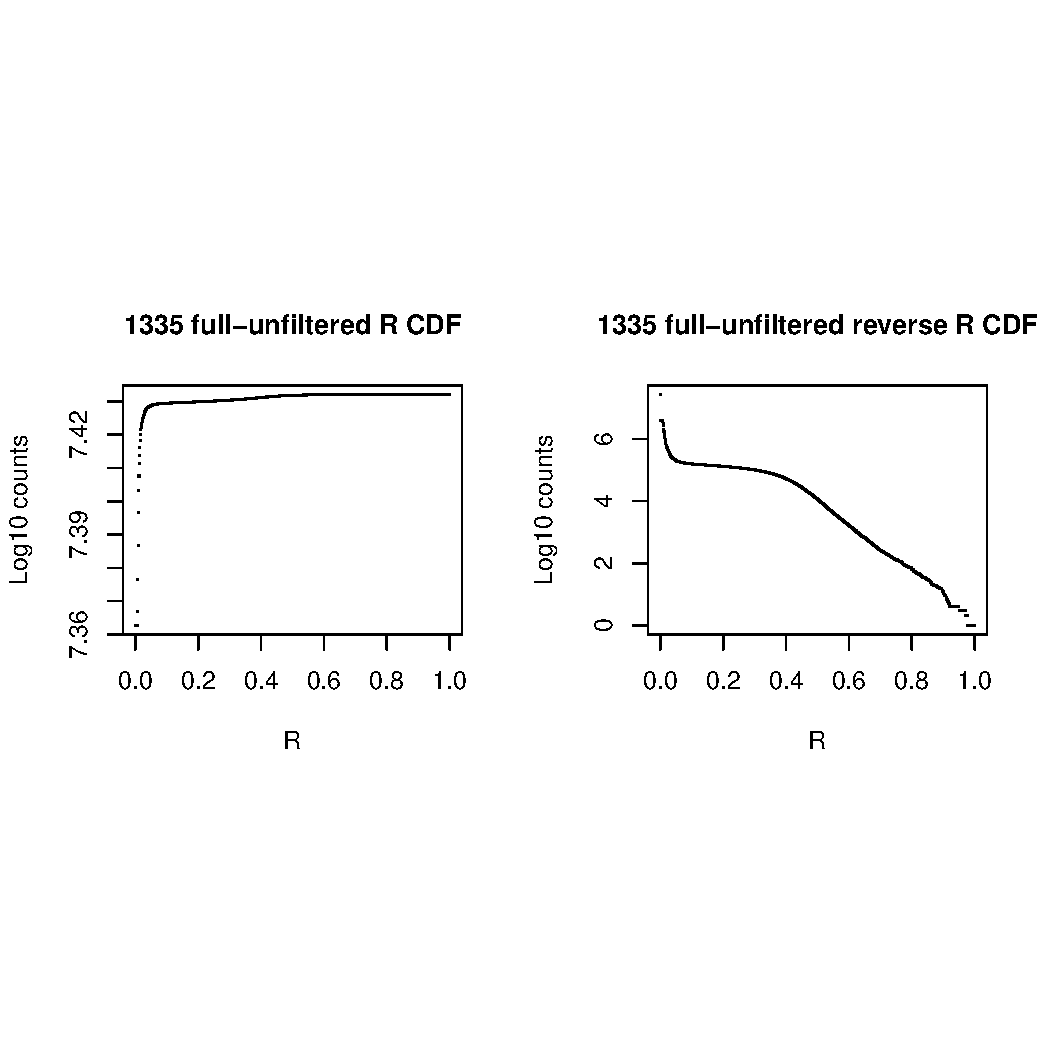
\includegraphics[width=\maxwidth]{FigS7-hwe-histo-figs-knitr/unnamed-chunk-10-14} 
\begin{kframe}\begin{verbatim}
#      [,1]    [,2]    [,3]    [,4]    [,5]  [,6]    [,7]    [,8]     [,9]     [,10]    [,11] 
# [1,] "blue"  "nm3"   "nm3x"  "nm3hi" "red" "black" "green" "orange" "ornghi" "nzgrey" "grey"
# [2,] "15569" "13053" "26106" "20"    NA    NA      NA      "26106"  "20"     NA       NA    
# FigS7-hwe-histo-figs-mine/S7-Chr1-unfiltered-1007.pdf written; 301-bin histo follows:
\end{verbatim}
\end{kframe}
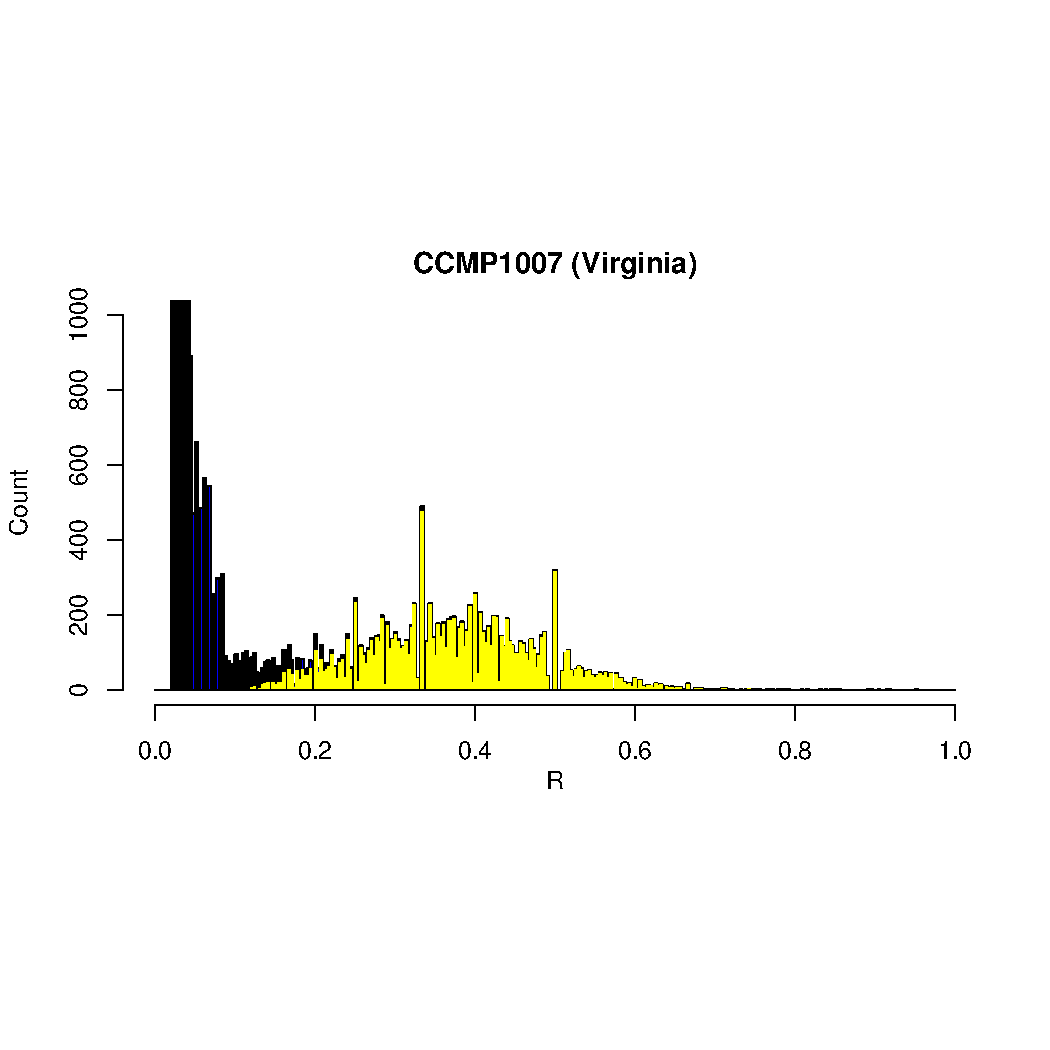
\includegraphics[width=\maxwidth]{FigS7-hwe-histo-figs-knitr/unnamed-chunk-10-15} 
\begin{kframe}\begin{verbatim}
#      [,1]    [,2]    [,3]   [,4]    [,5]  [,6]    [,7]    [,8]     [,9]     [,10]    [,11] 
# [1,] "blue"  "nm3"   "nm3x" "nm3hi" "red" "black" "green" "orange" "ornghi" "nzgrey" "grey"
# [2,] "15569" "15305" NA     "0"     NA    NA      NA      NA       NA       NA       NA
# 
# homnr:het ratios vs mod.humpth lo x hi, Chr1-unfiltered :
#       hi
# lo     0.7 0.75 0.76 0.77 0.78 0.79 0.8 0.85 0.9
#   0.1   NA   NA   NA   NA   NA   NA  NA   NA  NA
#   0.15  NA   NA   NA   NA   NA   NA  NA   NA  NA
#   0.16  NA   NA   NA   NA   NA   NA  NA   NA  NA
#   0.17  NA   NA   NA   NA   NA   NA  NA   NA  NA
#   0.18  NA   NA   NA   NA   NA   NA  NA   NA  NA
#   0.19  NA   NA   NA   NA   NA   NA  NA   NA  NA
#   0.2   NA   NA   NA   NA   NA   NA  NA   NA  NA
#   0.25  NA   NA   NA   NA   NA   NA  NA   NA  NA
# 
# 
# 1012 coverage summary for retained sites:
#    Min. 1st Qu.  Median    Mean 3rd Qu.    Max. 
#   45.00   56.00   66.00   66.54   76.00   92.00 
# FigS7-hwe-histo-figs-mine/S7-Chr1-unfiltered-1012.pdf :
#   based on 2318247 positions with coverage in [ 44.24661 , 92.15455 ]
\end{verbatim}
\end{kframe}
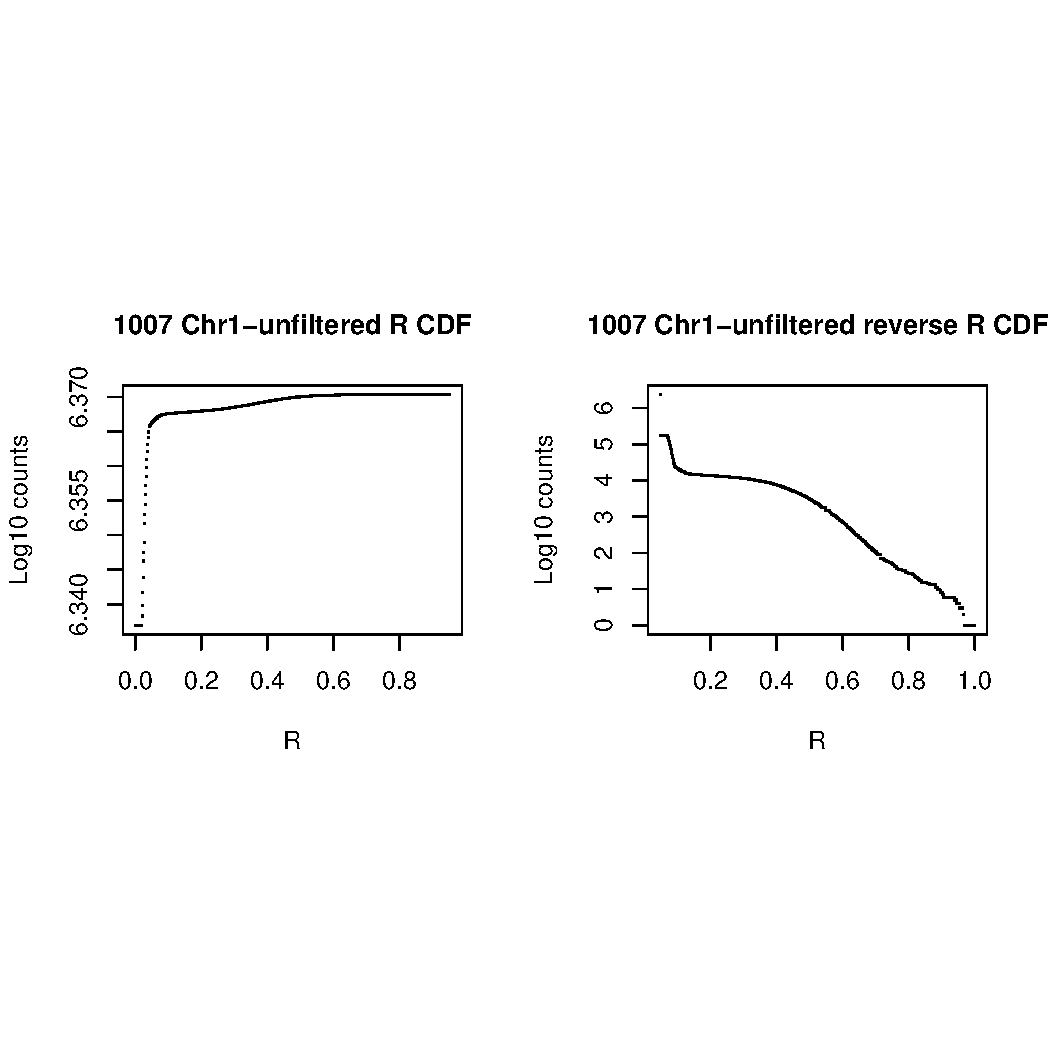
\includegraphics[width=\maxwidth]{FigS7-hwe-histo-figs-knitr/unnamed-chunk-10-16} 
\begin{kframe}\begin{verbatim}
#      [,1]    [,2]    [,3]    [,4]    [,5]  [,6]    [,7]    [,8]     [,9]     [,10]    [,11] 
# [1,] "blue"  "nm3"   "nm3x"  "nm3hi" "red" "black" "green" "orange" "ornghi" "nzgrey" "grey"
# [2,] "17190" "12973" "25946" "22"    NA    NA      NA      "25946"  "22"     NA       NA    
# FigS7-hwe-histo-figs-mine/S7-Chr1-unfiltered-1012.pdf written; 301-bin histo follows:
\end{verbatim}
\end{kframe}
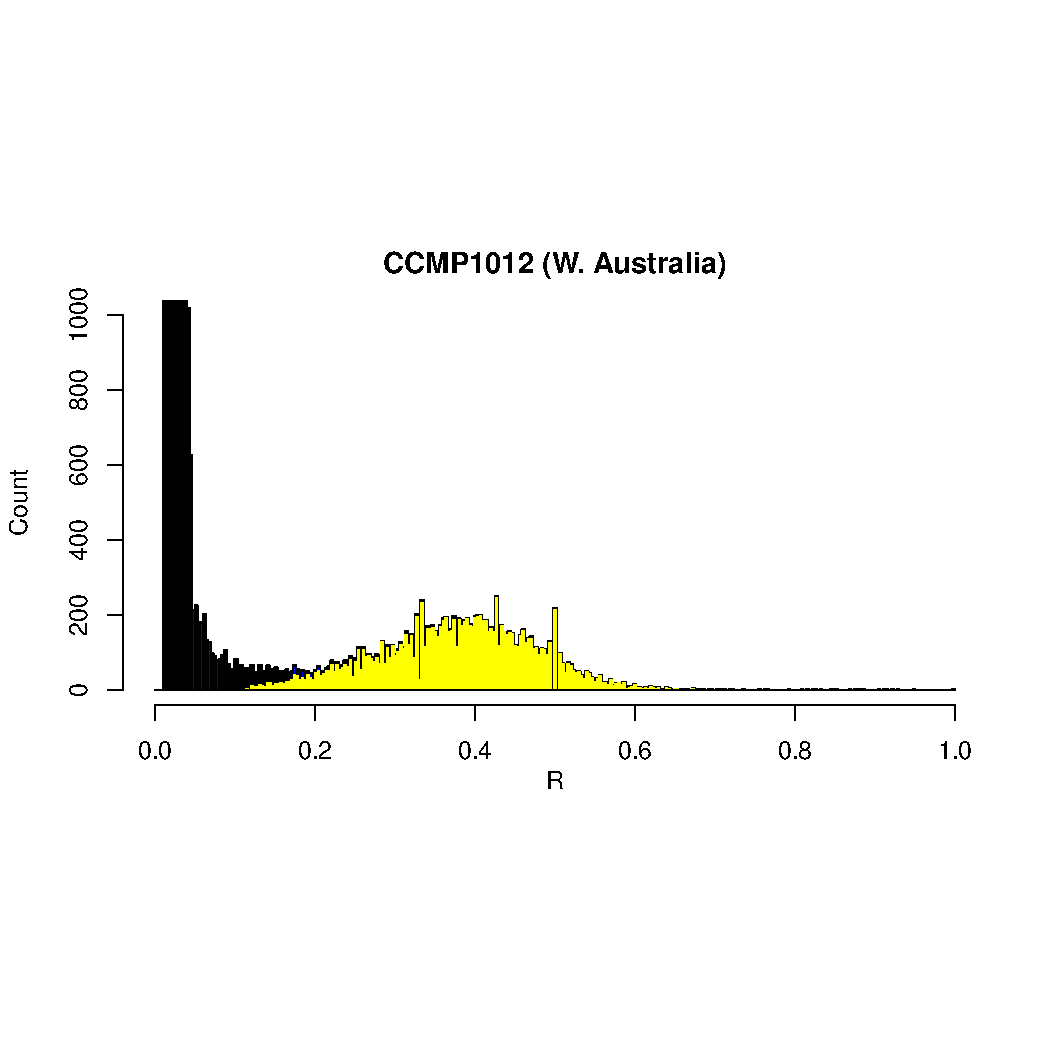
\includegraphics[width=\maxwidth]{FigS7-hwe-histo-figs-knitr/unnamed-chunk-10-17} 
\begin{kframe}\begin{verbatim}
#      [,1]    [,2]    [,3]   [,4]    [,5]  [,6]    [,7]    [,8]     [,9]     [,10]    [,11] 
# [1,] "blue"  "nm3"   "nm3x" "nm3hi" "red" "black" "green" "orange" "ornghi" "nzgrey" "grey"
# [2,] "17190" "17054" NA     "0"     NA    NA      NA      NA       NA       NA       NA
# 
# homnr:het ratios vs mod.humpth lo x hi, Chr1-unfiltered :
#       hi
# lo          0.7   0.75     0.76     0.77     0.78     0.79      0.8     0.85      0.9
#   0.1  408.5429 572.36 596.2500 650.5455 650.5455 650.5455 681.5714 954.6000 2046.714
#   0.15 384.6000 538.84 561.3333 612.4545 612.4545 612.4545 641.6667 898.7333 1927.000
#   0.16 380.0857 532.52 554.7500 605.2727 605.2727 605.2727 634.1429 888.2000 1904.429
#   0.17 376.2000 527.08 549.0833 599.0909 599.0909 599.0909 627.6667 879.1333 1885.000
#   0.18 371.1714 520.04 541.7500 591.0909 591.0909 591.0909 619.2857 867.4000 1859.857
#   0.19 367.5714 515.00 536.5000 585.3636 585.3636 585.3636 613.2857 859.0000 1841.857
#   0.2  362.3714 507.72 528.9167 577.0909 577.0909 577.0909 604.6190 846.8667 1815.857
#   0.25 334.2571 468.36 487.9167 532.3636 532.3636 532.3636 557.7619 781.2667 1675.286
# 
# 
# 1013 coverage summary for retained sites:
#    Min. 1st Qu.  Median    Mean 3rd Qu.    Max. 
#   39.00   52.00   62.00   63.06   73.00   95.00 
# FigS7-hwe-histo-figs-mine/S7-Chr1-unfiltered-1013.pdf :
#   based on 2488707 positions with coverage in [ 38.1606 , 95.22118 ]
\end{verbatim}
\end{kframe}
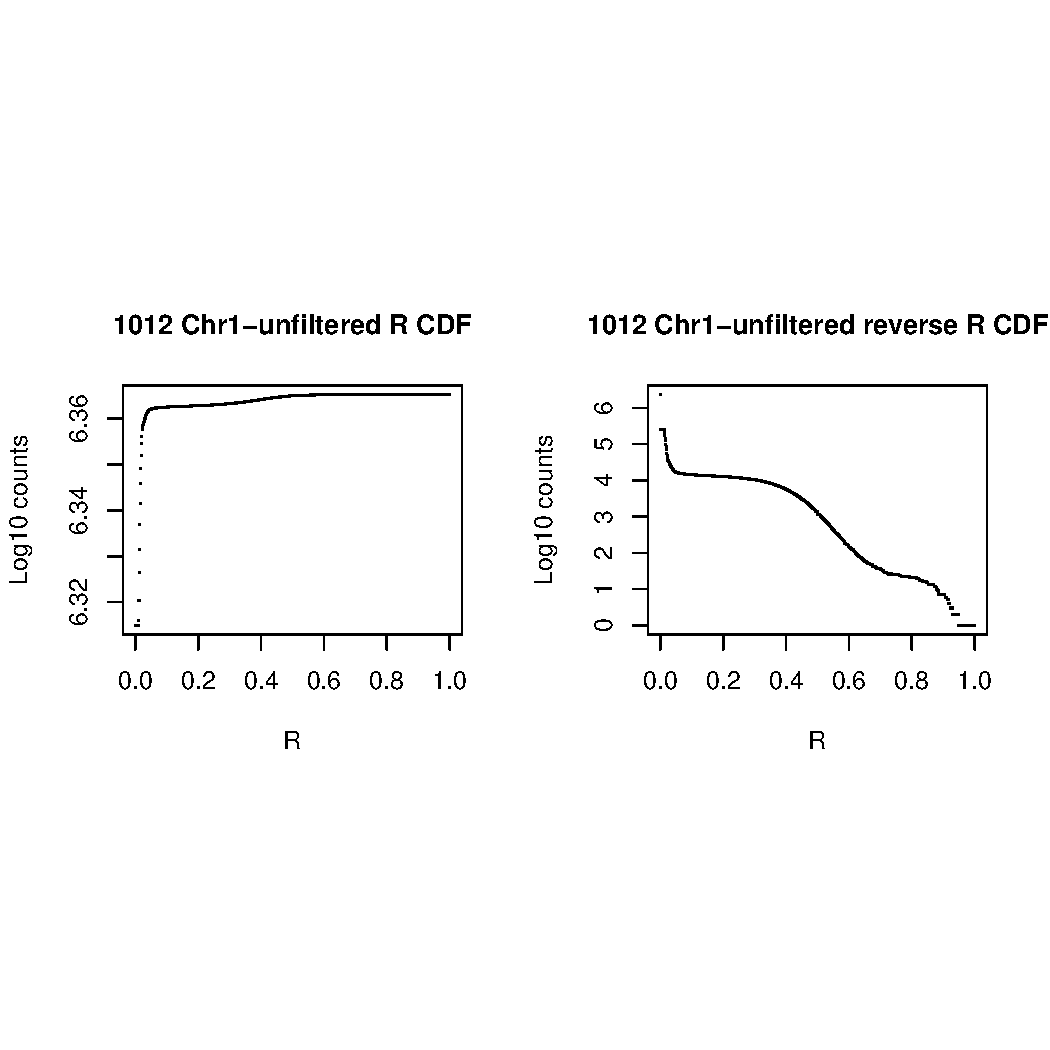
\includegraphics[width=\maxwidth]{FigS7-hwe-histo-figs-knitr/unnamed-chunk-10-18} 
\begin{kframe}\begin{verbatim}
#      [,1]    [,2]    [,3]    [,4]    [,5]  [,6]    [,7]    [,8]     [,9]     [,10]    [,11] 
# [1,] "blue"  "nm3"   "nm3x"  "nm3hi" "red" "black" "green" "orange" "ornghi" "nzgrey" "grey"
# [2,] "31142" "19774" "39548" "4389"  NA    NA      NA      "39548"  "4389"   NA       NA    
# FigS7-hwe-histo-figs-mine/S7-Chr1-unfiltered-1013.pdf written; 301-bin histo follows:
\end{verbatim}
\end{kframe}
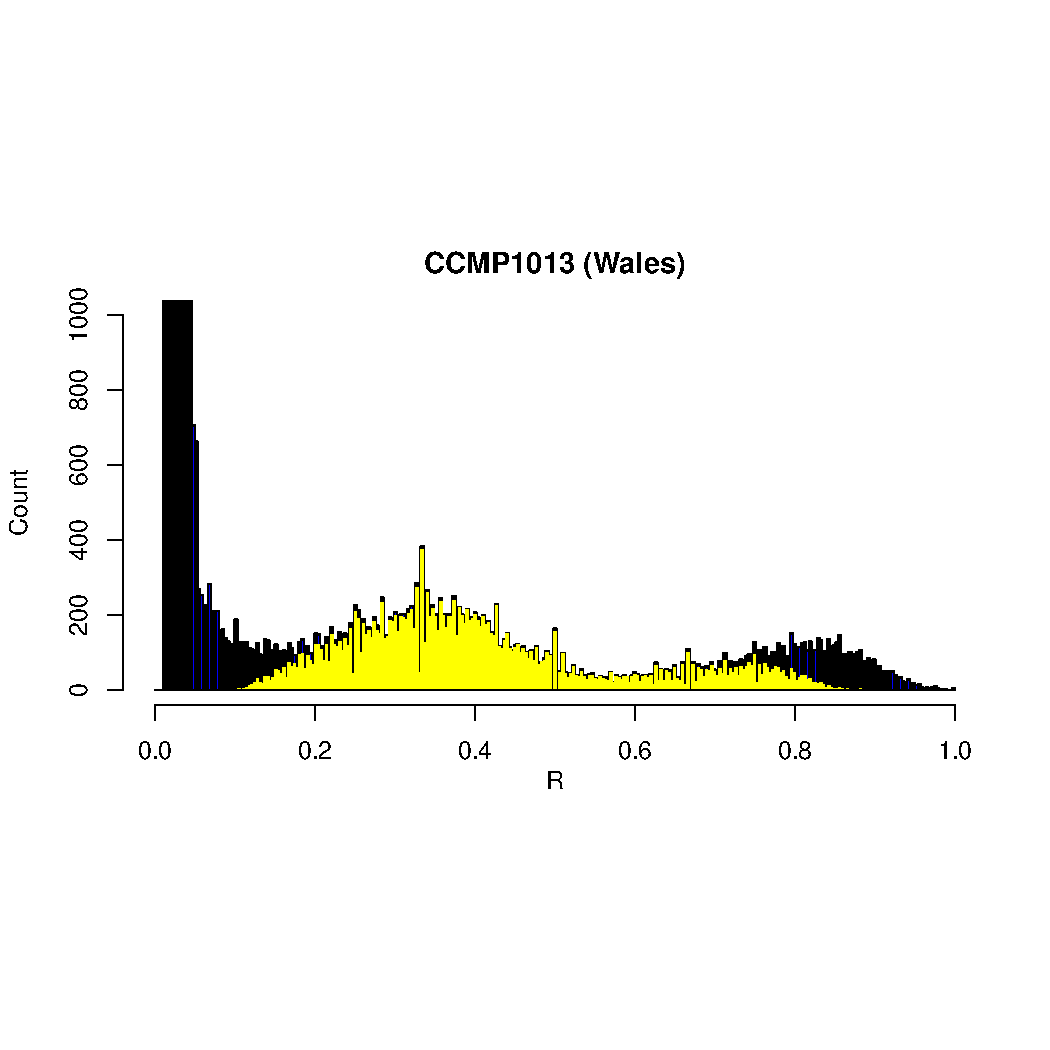
\includegraphics[width=\maxwidth]{FigS7-hwe-histo-figs-knitr/unnamed-chunk-10-19} 
\begin{kframe}\begin{verbatim}
#      [,1]    [,2]    [,3]   [,4]    [,5]  [,6]    [,7]    [,8]     [,9]     [,10]    [,11] 
# [1,] "blue"  "nm3"   "nm3x" "nm3hi" "red" "black" "green" "orange" "ornghi" "nzgrey" "grey"
# [2,] "31142" "23408" NA     "0"     NA    NA      NA      NA       NA       NA       NA
# 
# homnr:het ratios vs mod.humpth lo x hi, Chr1-unfiltered :
#       hi
# lo          0.7     0.75     0.76     0.77     0.78     0.79      0.8      0.85      0.9
#   0.1  3.225370 4.134443 4.354607 4.661746 5.064604 5.496008 6.182451 12.083821 41.75159
#   0.15 2.960183 3.812201 4.018548 4.306411 4.683985 5.088314 5.731675 11.262671 39.06847
#   0.16 2.911394 3.752916 3.956721 4.241038 4.613960 5.013308 5.648743 11.111598 38.57484
#   0.17 2.867328 3.699369 3.900878 4.181991 4.550712 4.945560 5.573836 10.975146 38.12898
#   0.18 2.816336 3.637407 3.836258 4.113665 4.477524 4.867167 5.487159 10.817251 37.61306
#   0.19 2.769122 3.580034 3.776426 4.050401 4.409758 4.794580 5.406902 10.671053 37.13535
#   0.2  2.699402 3.495315 3.688073 3.956980 4.309691 4.687394 5.288390 10.455166 36.42994
#   0.25 2.383223 3.111111 3.287395 3.533319 3.855884 4.201307 4.750936  9.476121 33.23089
# 
# 
# 1014 coverage summary for retained sites:
#    Min. 1st Qu.  Median    Mean 3rd Qu.    Max. 
#   20.00   25.00   30.00   29.96   35.00   42.00 
# FigS7-hwe-histo-figs-mine/S7-Chr1-unfiltered-1014.pdf :
#   based on 2253119 positions with coverage in [ 19.6778 , 42.85484 ]
\end{verbatim}
\end{kframe}
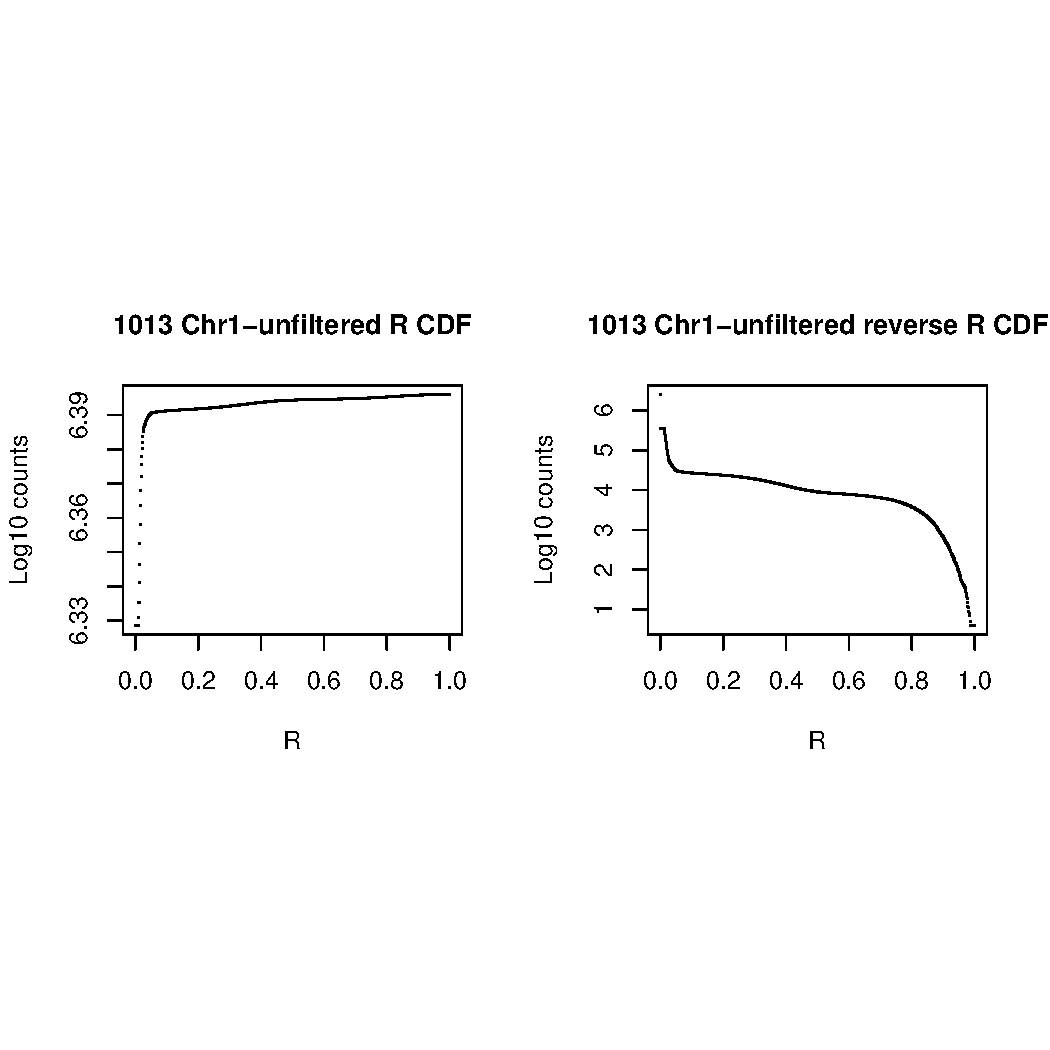
\includegraphics[width=\maxwidth]{FigS7-hwe-histo-figs-knitr/unnamed-chunk-10-20} 
\begin{kframe}\begin{verbatim}
#      [,1]    [,2]   [,3]    [,4]    [,5]  [,6]    [,7]    [,8]     [,9]     [,10]    [,11] 
# [1,] "blue"  "nm3"  "nm3x"  "nm3hi" "red" "black" "green" "orange" "ornghi" "nzgrey" "grey"
# [2,] "11144" "5903" "11806" "1"     NA    NA      NA      "11806"  "1"      NA       NA    
# FigS7-hwe-histo-figs-mine/S7-Chr1-unfiltered-1014.pdf written; 301-bin histo follows:
\end{verbatim}
\end{kframe}
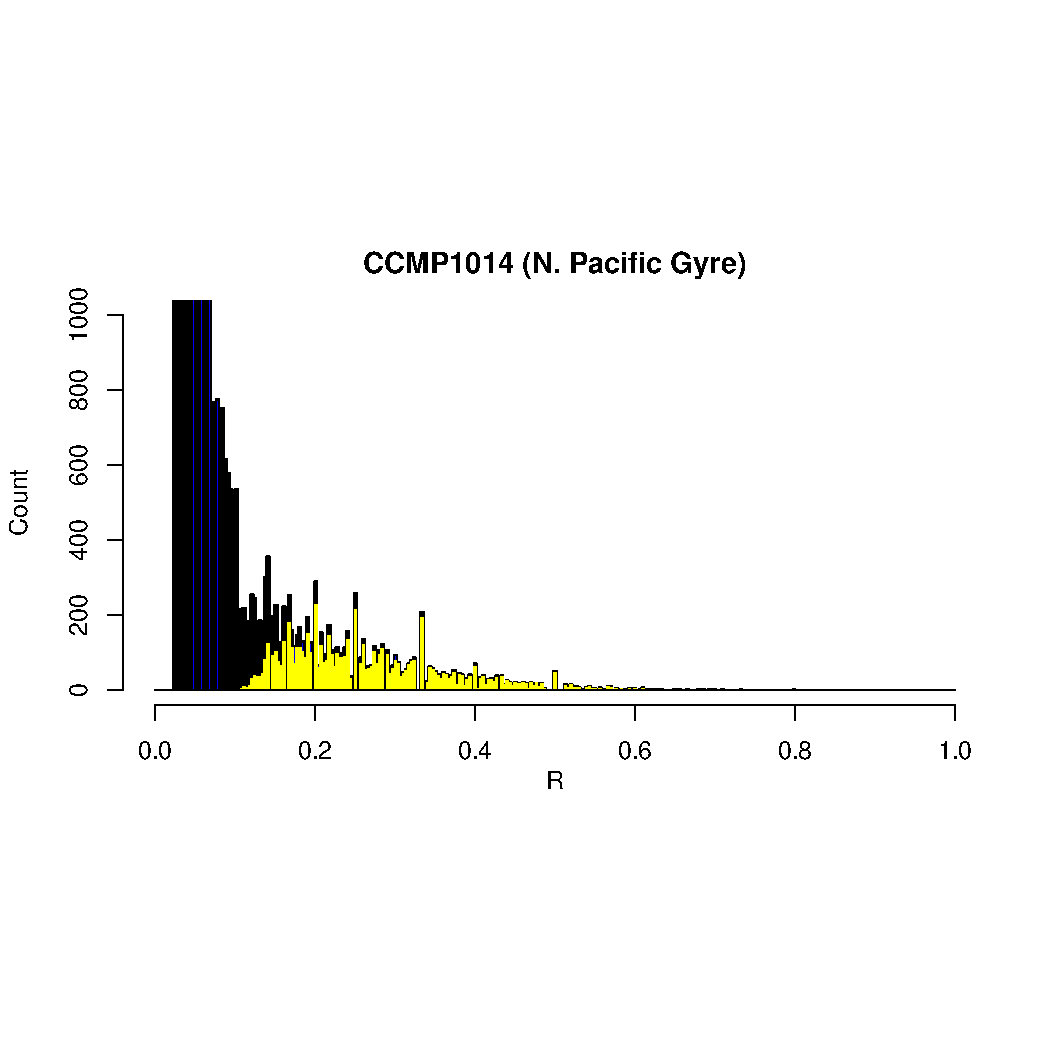
\includegraphics[width=\maxwidth]{FigS7-hwe-histo-figs-knitr/unnamed-chunk-10-21} 
\begin{kframe}\begin{verbatim}
#      [,1]    [,2]    [,3]   [,4]    [,5]  [,6]    [,7]    [,8]     [,9]     [,10]    [,11] 
# [1,] "blue"  "nm3"   "nm3x" "nm3hi" "red" "black" "green" "orange" "ornghi" "nzgrey" "grey"
# [2,] "11144" "11110" NA     "0"     NA    NA      NA      NA       NA       NA       NA
# 
# homnr:het ratios vs mod.humpth lo x hi, Chr1-unfiltered :
#       hi
# lo     0.7 0.75 0.76 0.77 0.78 0.79 0.8 0.85 0.9
#   0.1   NA   NA   NA   NA   NA   NA  NA   NA  NA
#   0.15  NA   NA   NA   NA   NA   NA  NA   NA  NA
#   0.16  NA   NA   NA   NA   NA   NA  NA   NA  NA
#   0.17  NA   NA   NA   NA   NA   NA  NA   NA  NA
#   0.18  NA   NA   NA   NA   NA   NA  NA   NA  NA
#   0.19  NA   NA   NA   NA   NA   NA  NA   NA  NA
#   0.2   NA   NA   NA   NA   NA   NA  NA   NA  NA
#   0.25  NA   NA   NA   NA   NA   NA  NA   NA  NA
# 
# 
# 1015 coverage summary for retained sites:
#    Min. 1st Qu.  Median    Mean 3rd Qu.    Max. 
#   39.00   49.00   57.00   57.65   66.00   80.00 
# FigS7-hwe-histo-figs-mine/S7-Chr1-unfiltered-1015.pdf :
#   based on 2348252 positions with coverage in [ 38.26224 , 80.67859 ]
\end{verbatim}
\end{kframe}
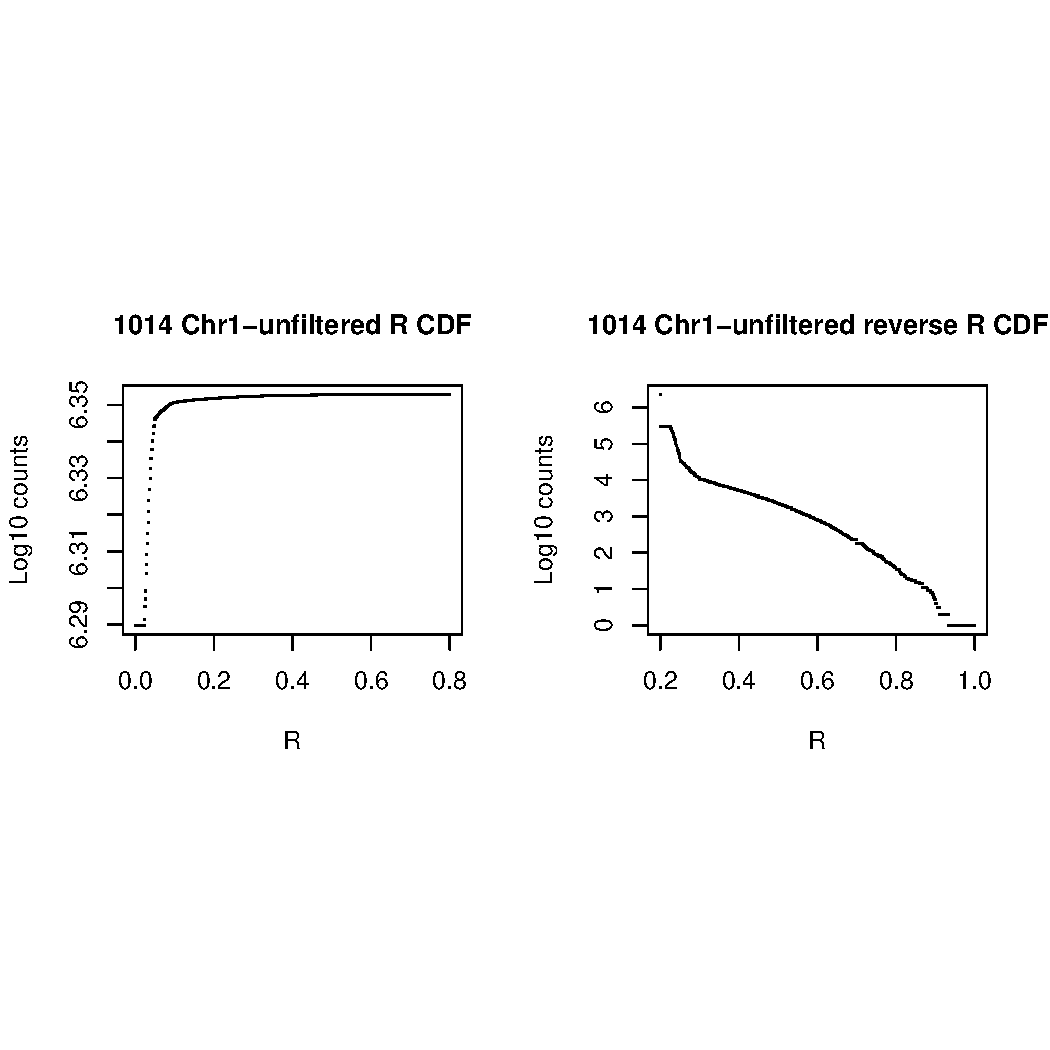
\includegraphics[width=\maxwidth]{FigS7-hwe-histo-figs-knitr/unnamed-chunk-10-22} 
\begin{kframe}\begin{verbatim}
#      [,1]    [,2]    [,3]    [,4]    [,5]  [,6]    [,7]    [,8]     [,9]     [,10]    [,11] 
# [1,] "blue"  "nm3"   "nm3x"  "nm3hi" "red" "black" "green" "orange" "ornghi" "nzgrey" "grey"
# [2,] "17265" "13575" "27150" "16"    NA    NA      NA      "27150"  "16"     NA       NA    
# FigS7-hwe-histo-figs-mine/S7-Chr1-unfiltered-1015.pdf written; 301-bin histo follows:
\end{verbatim}
\end{kframe}
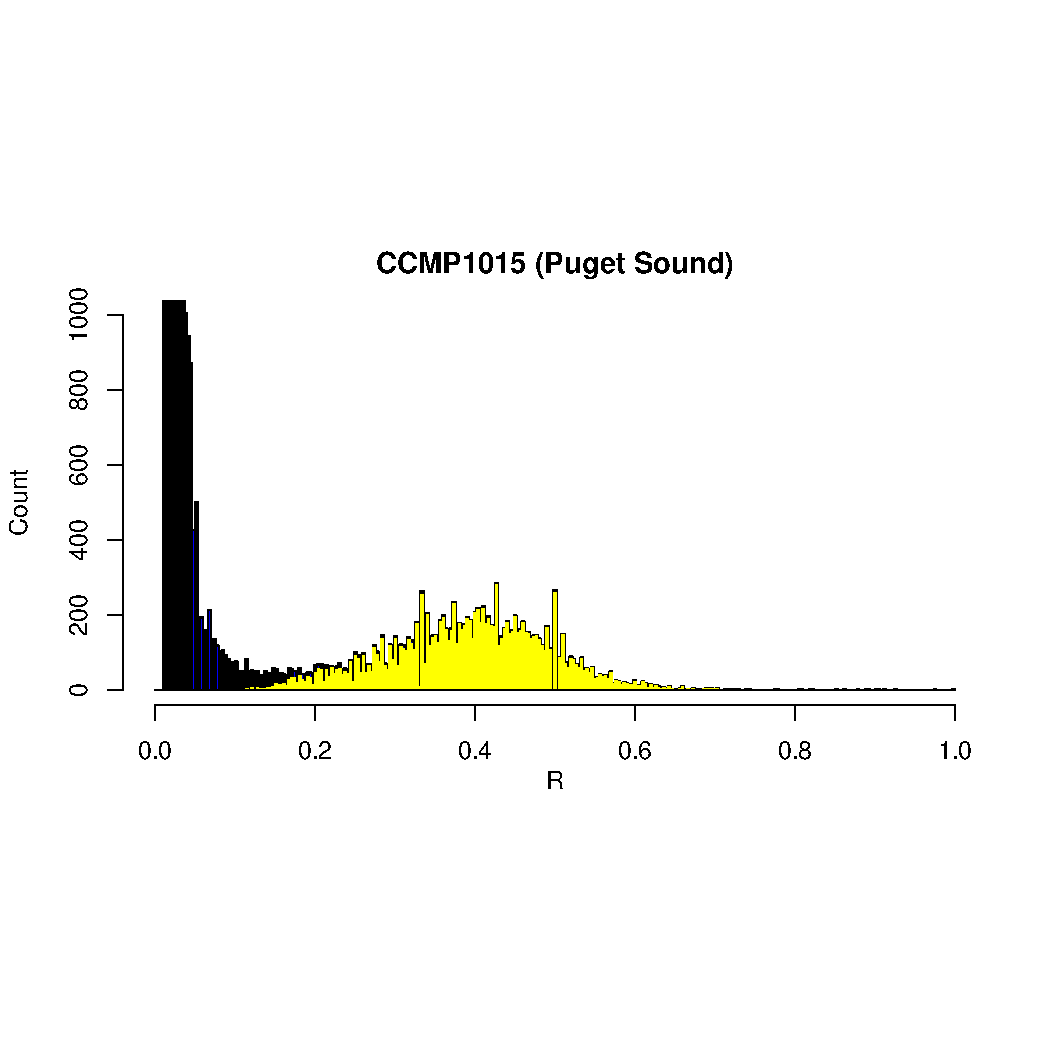
\includegraphics[width=\maxwidth]{FigS7-hwe-histo-figs-knitr/unnamed-chunk-10-23} 
\begin{kframe}\begin{verbatim}
#      [,1]    [,2]    [,3]   [,4]    [,5]  [,6]    [,7]    [,8]     [,9]     [,10]    [,11] 
# [1,] "blue"  "nm3"   "nm3x" "nm3hi" "red" "black" "green" "orange" "ornghi" "nzgrey" "grey"
# [2,] "17265" "17044" NA     "0"     NA    NA      NA      NA       NA       NA       NA
# 
# homnr:het ratios vs mod.humpth lo x hi, Chr1-unfiltered :
#       hi
# lo          0.7     0.75     0.76     0.77     0.78     0.79      0.8     0.85      0.9
#   0.1  462.2500 822.5556 822.5556 822.5556 925.5000 925.5000 925.5000 1234.333 2116.714
#   0.15 437.8438 779.1667 779.1667 779.1667 876.6875 876.6875 876.6875 1169.250 2005.143
#   0.16 433.4375 771.3333 771.3333 771.3333 867.8750 867.8750 867.8750 1157.500 1985.000
#   0.17 429.3750 764.1111 764.1111 764.1111 859.7500 859.7500 859.7500 1146.667 1966.429
#   0.18 424.6250 755.6667 755.6667 755.6667 850.2500 850.2500 850.2500 1134.000 1944.714
#   0.19 420.9688 749.1667 749.1667 749.1667 842.9375 842.9375 842.9375 1124.250 1928.000
#   0.2  415.6250 739.6667 739.6667 739.6667 832.2500 832.2500 832.2500 1110.000 1903.571
#   0.25 388.0625 690.6667 690.6667 690.6667 777.1250 777.1250 777.1250 1036.500 1777.571
# 
# 
# 3367 coverage summary for retained sites:
#    Min. 1st Qu.  Median    Mean 3rd Qu.    Max. 
#   41.00   53.00   62.00   61.89   70.00   84.00 
# FigS7-hwe-histo-figs-mine/S7-Chr1-unfiltered-3367.pdf :
#   based on 2440468 positions with coverage in [ 40.74172 , 84.02519 ]
\end{verbatim}
\end{kframe}
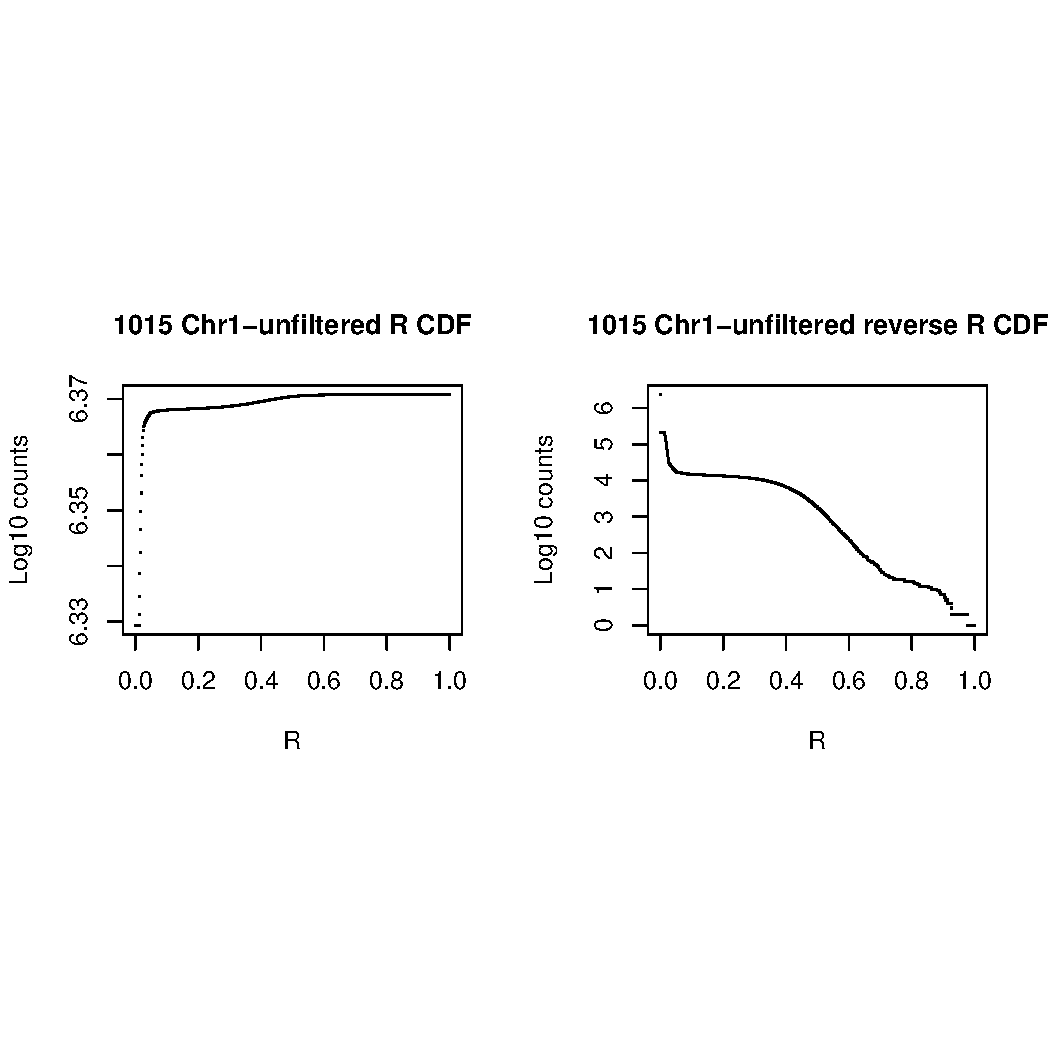
\includegraphics[width=\maxwidth]{FigS7-hwe-histo-figs-knitr/unnamed-chunk-10-24} 
\begin{kframe}\begin{verbatim}
#      [,1]    [,2]    [,3]    [,4]    [,5]  [,6]    [,7]    [,8]     [,9]     [,10]    [,11] 
# [1,] "blue"  "nm3"   "nm3x"  "nm3hi" "red" "black" "green" "orange" "ornghi" "nzgrey" "grey"
# [2,] "27475" "17108" "34216" "4791"  NA    NA      NA      "34216"  "4791"   NA       NA    
# FigS7-hwe-histo-figs-mine/S7-Chr1-unfiltered-3367.pdf written; 301-bin histo follows:
\end{verbatim}
\end{kframe}
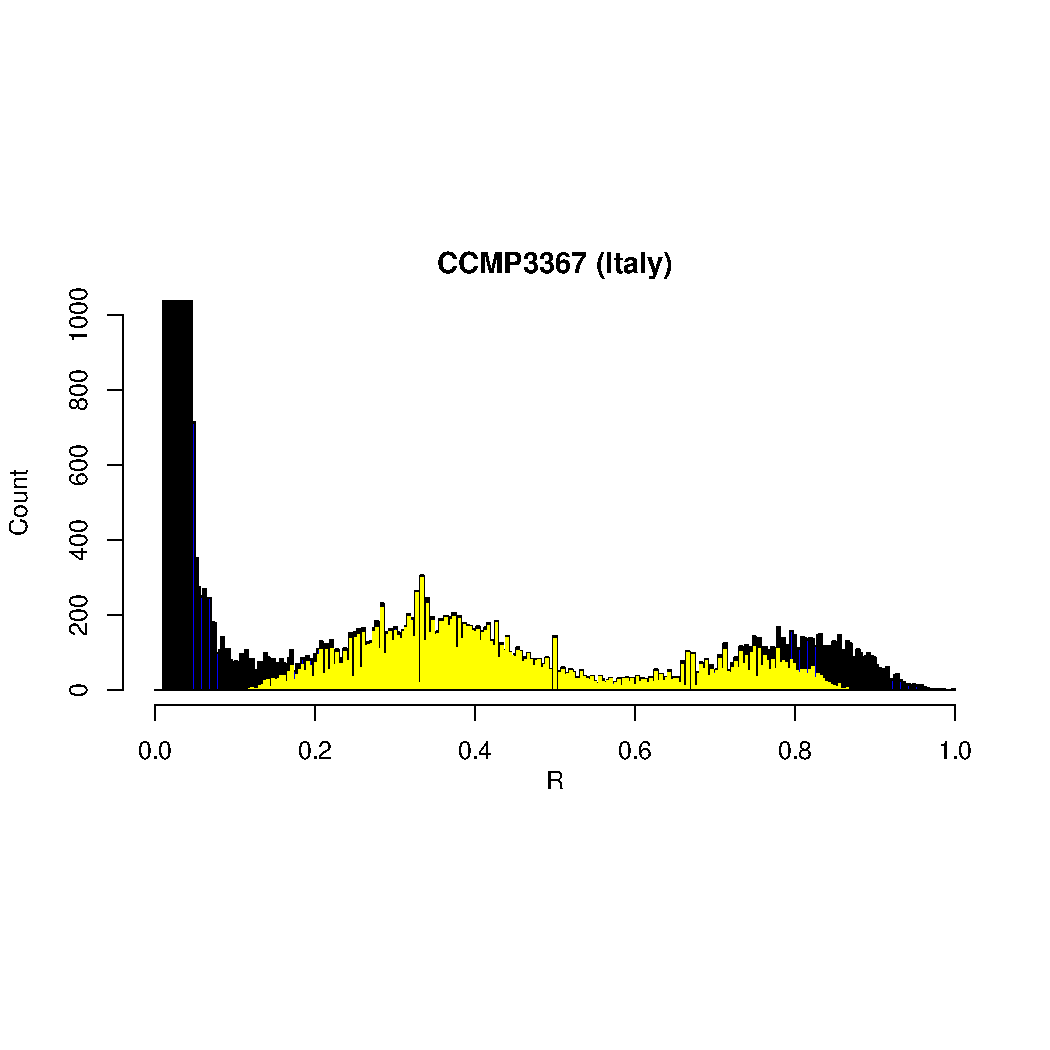
\includegraphics[width=\maxwidth]{FigS7-hwe-histo-figs-knitr/unnamed-chunk-10-25} 
\begin{kframe}\begin{verbatim}
#      [,1]    [,2]    [,3]   [,4]    [,5]  [,6]    [,7]    [,8]     [,9]     [,10]    [,11] 
# [1,] "blue"  "nm3"   "nm3x" "nm3hi" "red" "black" "green" "orange" "ornghi" "nzgrey" "grey"
# [2,] "27475" "19197" NA     "0"     NA    NA      NA      NA       NA       NA       NA
# 
# homnr:het ratios vs mod.humpth lo x hi, Chr1-unfiltered :
#       hi
# lo          0.7     0.75     0.76     0.77     0.78     0.79      0.8      0.85      0.9
#   0.1  2.374111 3.132404 3.330047 3.578267 3.915044 4.292280 4.875650 10.193959 39.34014
#   0.15 2.216216 2.939024 3.127419 3.364022 3.685039 4.044623 4.600694  9.670127 37.45238
#   0.16 2.182646 2.897909 3.084337 3.318471 3.636138 3.991968 4.542234  9.558754 37.05102
#   0.17 2.153627 2.862369 3.047097 3.279097 3.593867 3.946452 4.491702  9.462482 36.70408
#   0.18 2.122191 2.823868 3.006754 3.236441 3.548073 3.897144 4.436958  9.358188 36.32823
#   0.19 2.093172 2.788328 2.969514 3.197066 3.505802 3.851629 4.386426  9.261916 35.98129
#   0.2  2.048222 2.733275 2.911829 3.136074 3.440323 3.781124 4.308150  9.112789 35.44388
#   0.25 1.834708 2.471777 2.637824 2.846362 3.129300 3.446229 3.936339  8.404436 32.89116
# 
# 
# 1335 coverage summary for retained sites:
#    Min. 1st Qu.  Median    Mean 3rd Qu.    Max. 
#    71.0    92.0   105.0   104.7   118.0   136.0 
# FigS7-hwe-histo-figs-mine/S7-Chr1-unfiltered-1335.pdf :
#   based on 2357606 positions with coverage in [ 70.94551 , 136.8794 ]
\end{verbatim}
\end{kframe}
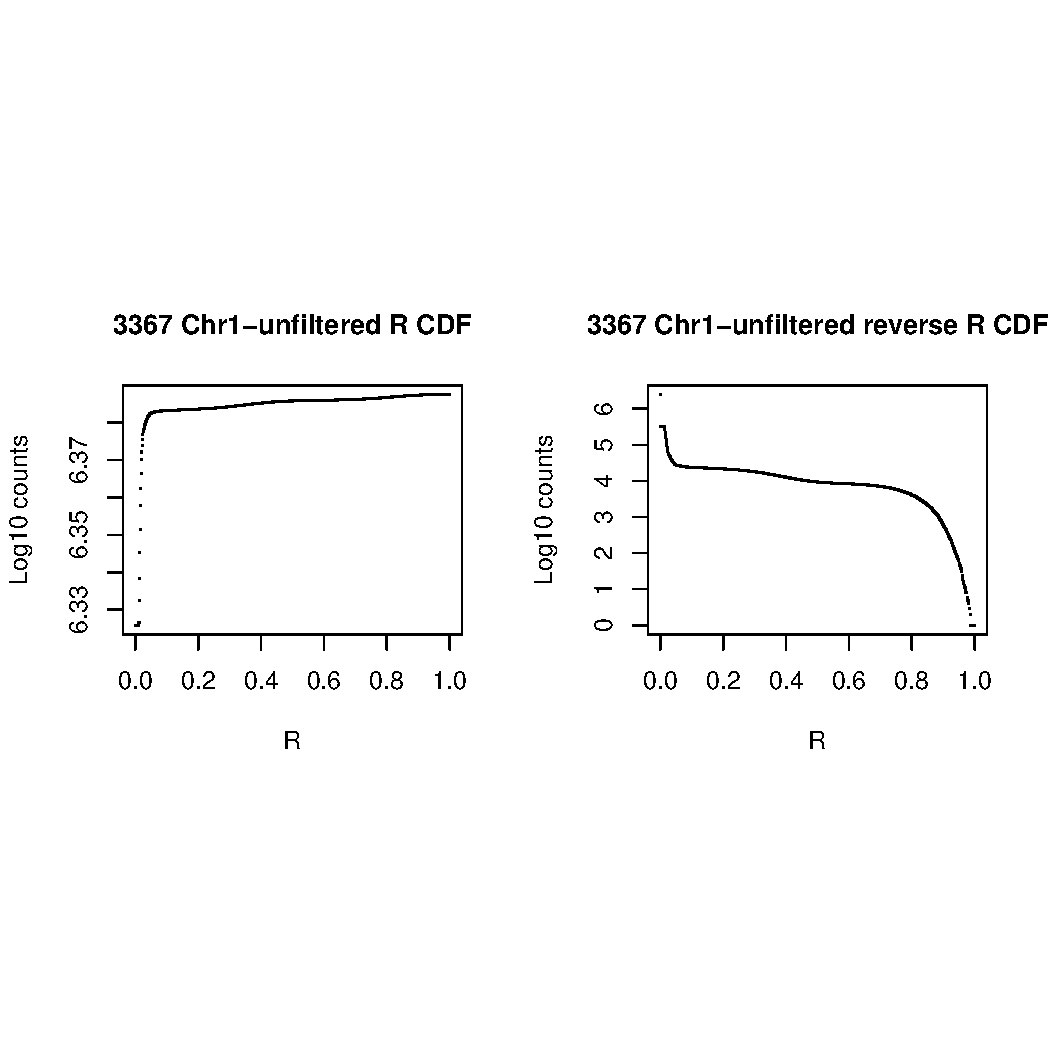
\includegraphics[width=\maxwidth]{FigS7-hwe-histo-figs-knitr/unnamed-chunk-10-26} 
\begin{kframe}\begin{verbatim}
#      [,1]    [,2]    [,3]    [,4]    [,5]  [,6]    [,7]    [,8]     [,9]     [,10]    [,11] 
# [1,] "blue"  "nm3"   "nm3x"  "nm3hi" "red" "black" "green" "orange" "ornghi" "nzgrey" "grey"
# [2,] "22527" "11598" "23196" "2"     NA    NA      NA      "23196"  "2"      NA       NA    
# FigS7-hwe-histo-figs-mine/S7-Chr1-unfiltered-1335.pdf written; 301-bin histo follows:
\end{verbatim}
\end{kframe}
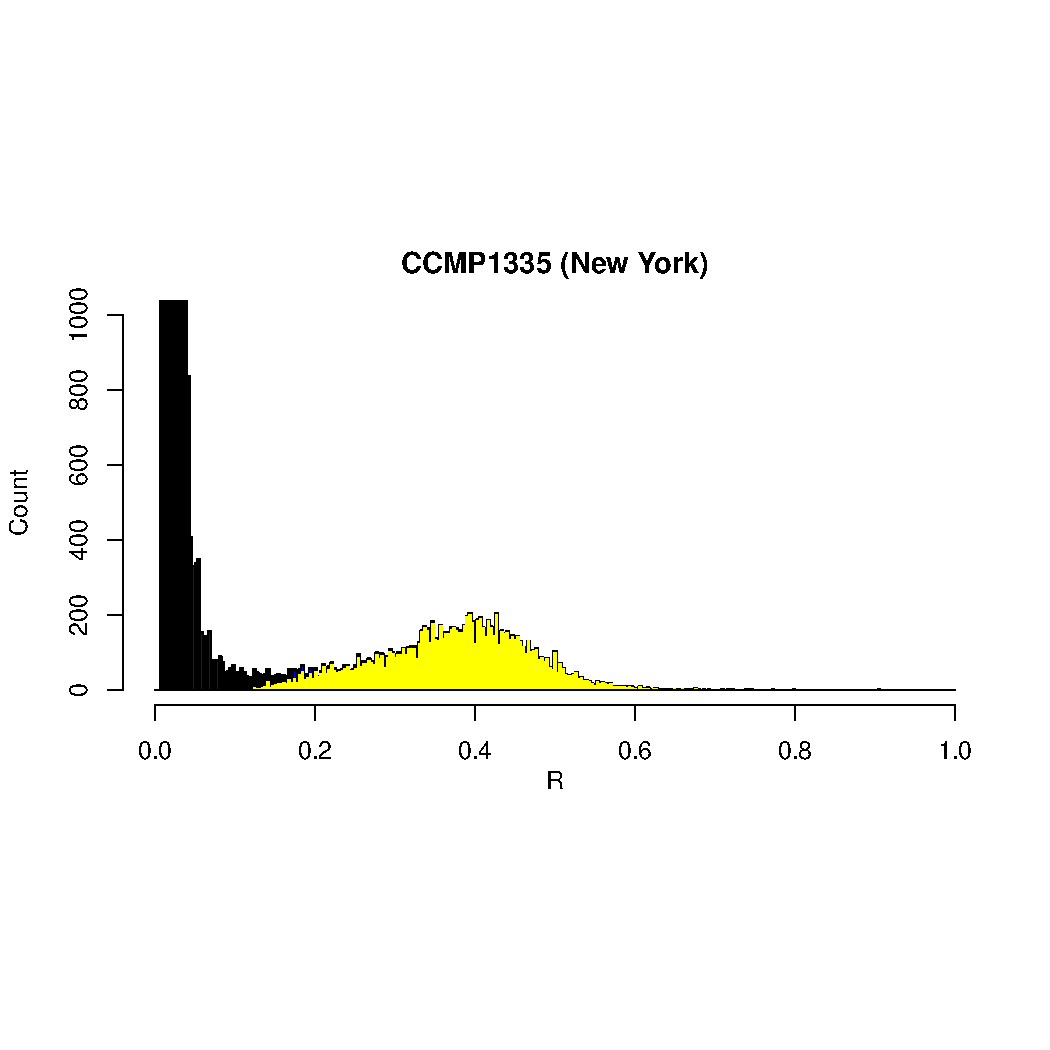
\includegraphics[width=\maxwidth]{FigS7-hwe-histo-figs-knitr/unnamed-chunk-10-27} 
\begin{kframe}\begin{verbatim}
#      [,1]    [,2]    [,3]   [,4]    [,5]  [,6]    [,7]    [,8]     [,9]     [,10]    [,11] 
# [1,] "blue"  "nm3"   "nm3x" "nm3hi" "red" "black" "green" "orange" "ornghi" "nzgrey" "grey"
# [2,] "22527" "22453" NA     "0"     NA    NA      NA      NA       NA       NA       NA
# 
# homnr:het ratios vs mod.humpth lo x hi, Chr1-unfiltered :
#       hi
# lo     0.7 0.75 0.76 0.77 0.78 0.79 0.8 0.85 0.9
#   0.1   NA   NA   NA   NA   NA   NA  NA   NA  NA
#   0.15  NA   NA   NA   NA   NA   NA  NA   NA  NA
#   0.16  NA   NA   NA   NA   NA   NA  NA   NA  NA
#   0.17  NA   NA   NA   NA   NA   NA  NA   NA  NA
#   0.18  NA   NA   NA   NA   NA   NA  NA   NA  NA
#   0.19  NA   NA   NA   NA   NA   NA  NA   NA  NA
#   0.2   NA   NA   NA   NA   NA   NA  NA   NA  NA
#   0.25  NA   NA   NA   NA   NA   NA  NA   NA  NA
# 
# 
# 
# ***
# *
# * Processing full-qfiltered 
# *
# ***
# full-qfiltered coverage stats:
#                    1007     1012     1013      1014     1015     3367     1335
# cov.means.all 28.706227 51.71471 45.68265 13.865883 50.24790 45.84290 83.66328
# cov.sigs.all  23.301651 36.71234 33.11370 11.514173 40.94410 34.27808 54.09077
# cov.means     28.275029 51.32497 45.40363 13.726105 48.78800 44.80421 81.88238
# cov.sigs      21.247546 35.10949 31.83052 11.227217 31.84672 29.32831 44.17400
# cov.min        7.027483 16.21548 13.57311  2.498888 16.94128 15.47590 37.70838
# 
# 
# 1007 coverage summary for retained sites:
#    Min. 1st Qu.  Median    Mean 3rd Qu.    Max. 
#    8.00   20.00   26.00   26.73   33.00   49.00 
# FigS7-hwe-histo-figs-mine/S7-full-qfiltered-1007chronly.pdf :
#   based on 28942481 positions with coverage in [ 7.027483 , 49.52257 ]
\end{verbatim}
\end{kframe}
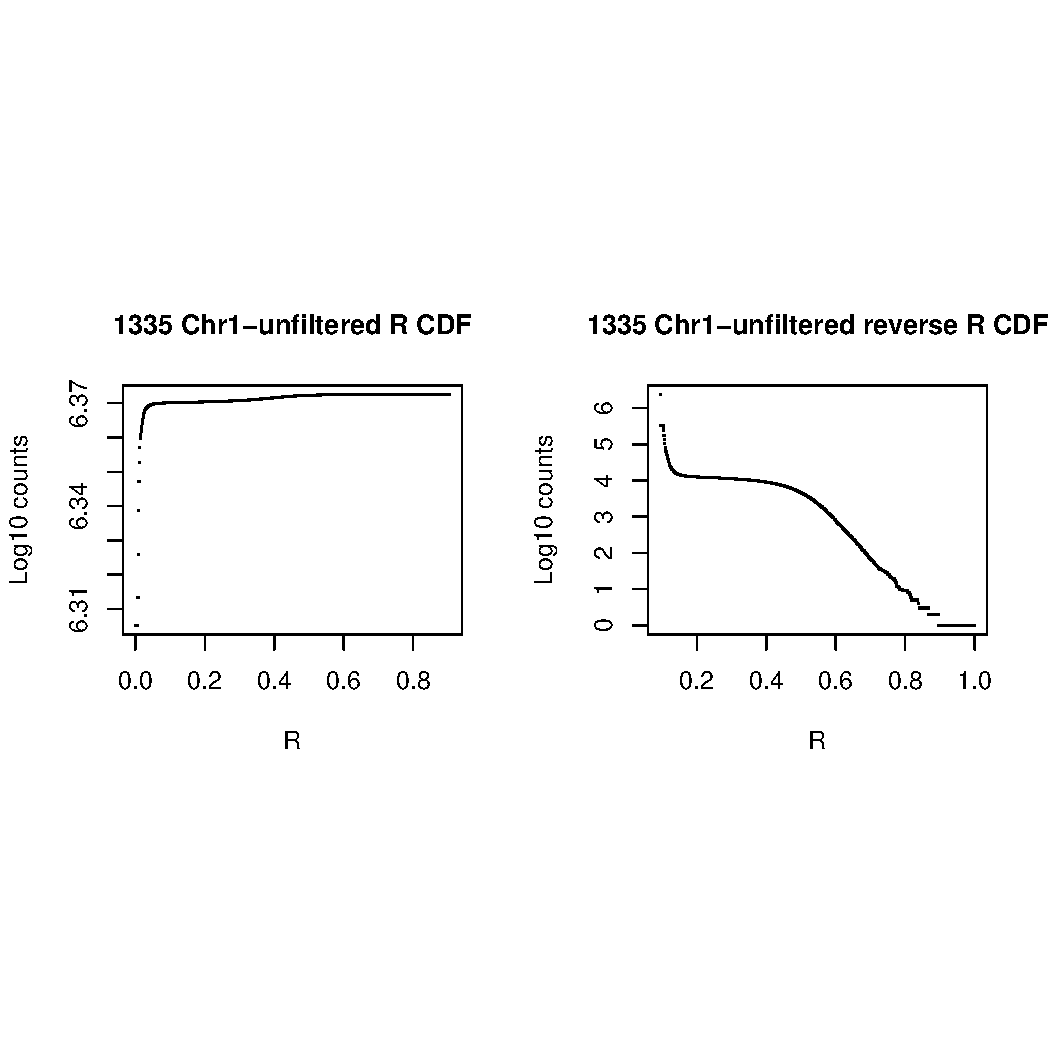
\includegraphics[width=\maxwidth]{FigS7-hwe-histo-figs-knitr/unnamed-chunk-10-28} 
\begin{kframe}\begin{verbatim}
#      [,1]     [,2]     [,3]     [,4]    [,5]  [,6]    [,7]    [,8]     [,9]     [,10]    [,11] 
# [1,] "blue"   "nm3"    "nm3x"   "nm3hi" "red" "black" "green" "orange" "ornghi" "nzgrey" "grey"
# [2,] "188959" "159187" "318374" "12048" NA    NA      NA      "318374" "12048"  NA       NA    
# FigS7-hwe-histo-figs-mine/S7-full-qfiltered-1007chronly.pdf written; 301-bin histo follows:
\end{verbatim}
\end{kframe}
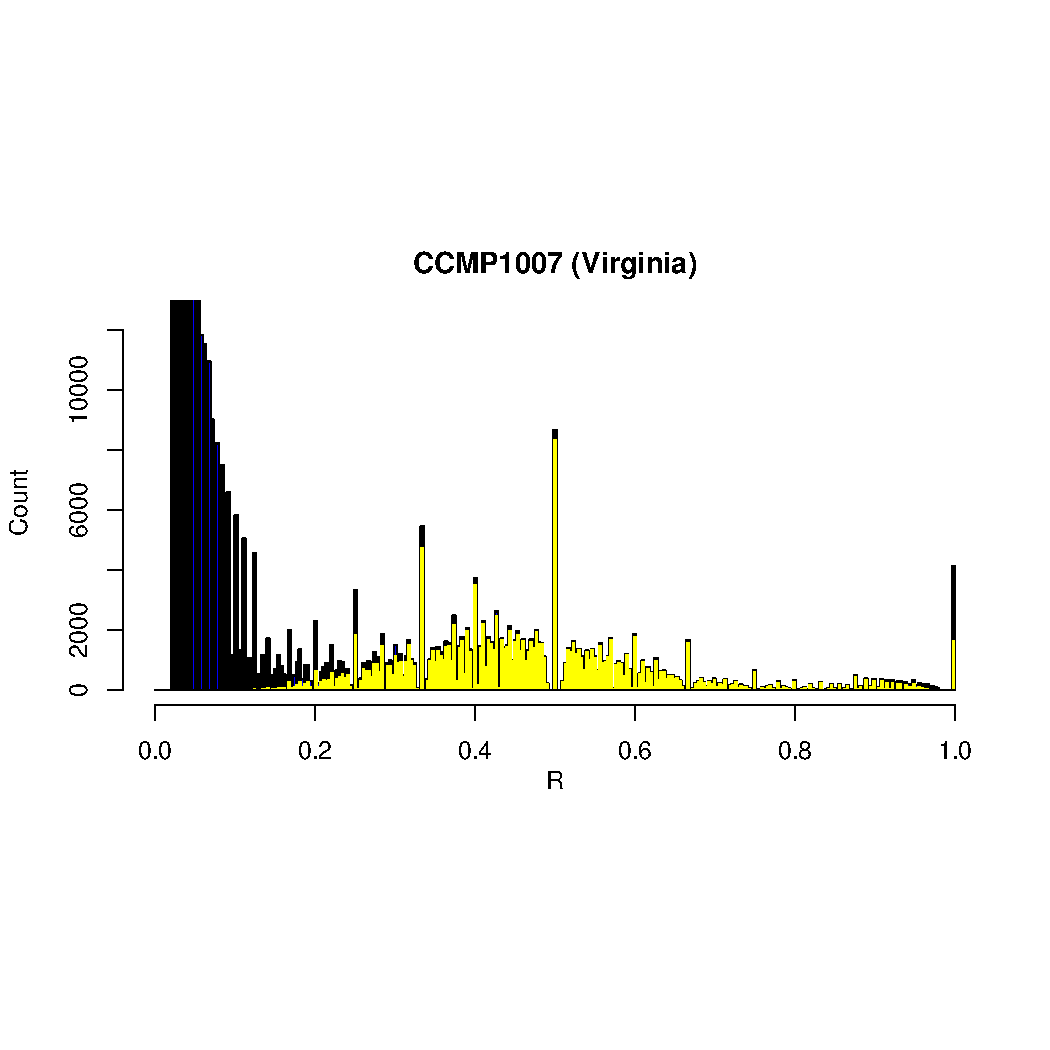
\includegraphics[width=\maxwidth]{FigS7-hwe-histo-figs-knitr/unnamed-chunk-10-29} 
\begin{kframe}\begin{verbatim}
#      [,1]     [,2]     [,3]   [,4]    [,5]  [,6]    [,7]    [,8]     [,9]     [,10]    [,11] 
# [1,] "blue"   "nm3"    "nm3x" "nm3hi" "red" "black" "green" "orange" "ornghi" "nzgrey" "grey"
# [2,] "188959" "160780" NA     "0"     NA    NA      NA      NA       NA       NA       NA
# 
# homnr:het ratios vs mod.humpth lo x hi, full-qfiltered :
#       hi
# lo           0.7     0.75     0.76     0.77     0.78     0.79      0.8     0.85      0.9
#   0.1  11.813491 14.53150 14.67976 15.13031 15.61716 15.98474 16.56226 18.46605 23.24132
#   0.15 10.533184 12.97962 13.11306 13.51859 13.95680 14.28765 14.80747 16.52103 20.81916
#   0.16 10.379156 12.79292 12.92458 13.32469 13.75705 14.08348 14.59635 16.28703 20.52776
#   0.17 10.229859 12.61195 12.74188 13.13675 13.56343 13.88558 14.39173 16.06022 20.24531
#   0.18 10.112212 12.46935 12.59792 12.98865 13.41086 13.72964 14.23048 15.88150 20.02274
#   0.19  9.954540 12.27823 12.40498 12.79016 13.20638 13.52064 14.01437 15.64196 19.72445
#   0.2   9.734079 12.01101 12.13520 12.51264 12.92048 13.22841 13.71221 15.30704 19.30737
#   0.25  8.947123 11.05712 11.17221 11.52197 11.89992 12.18527 12.63360 14.11151 17.81856
# 
# 
# 1012 coverage summary for retained sites:
#    Min. 1st Qu.  Median    Mean 3rd Qu.    Max. 
#   17.00   36.00   48.00   48.45   60.00   86.00 
# FigS7-hwe-histo-figs-mine/S7-full-qfiltered-1012chronly.pdf :
#   based on 28136229 positions with coverage in [ 16.21548 , 86.43446 ]
\end{verbatim}
\end{kframe}
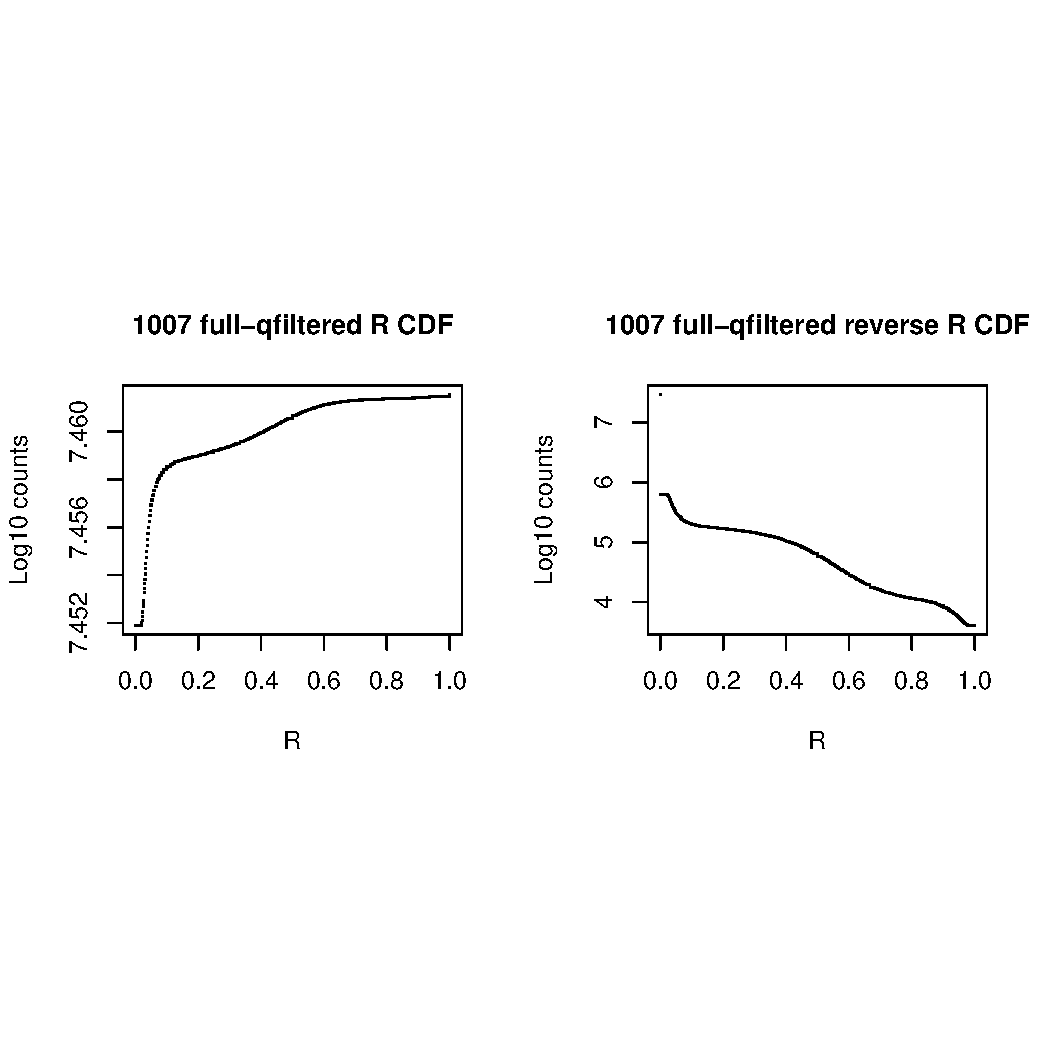
\includegraphics[width=\maxwidth]{FigS7-hwe-histo-figs-knitr/unnamed-chunk-10-30} 
\begin{kframe}\begin{verbatim}
#      [,1]     [,2]     [,3]     [,4]    [,5]  [,6]    [,7]    [,8]     [,9]     [,10]    [,11] 
# [1,] "blue"   "nm3"    "nm3x"   "nm3hi" "red" "black" "green" "orange" "ornghi" "nzgrey" "grey"
# [2,] "203028" "158178" "316356" "9952"  NA    NA      NA      "316356" "9952"   NA       NA    
# FigS7-hwe-histo-figs-mine/S7-full-qfiltered-1012chronly.pdf written; 301-bin histo follows:
\end{verbatim}
\end{kframe}
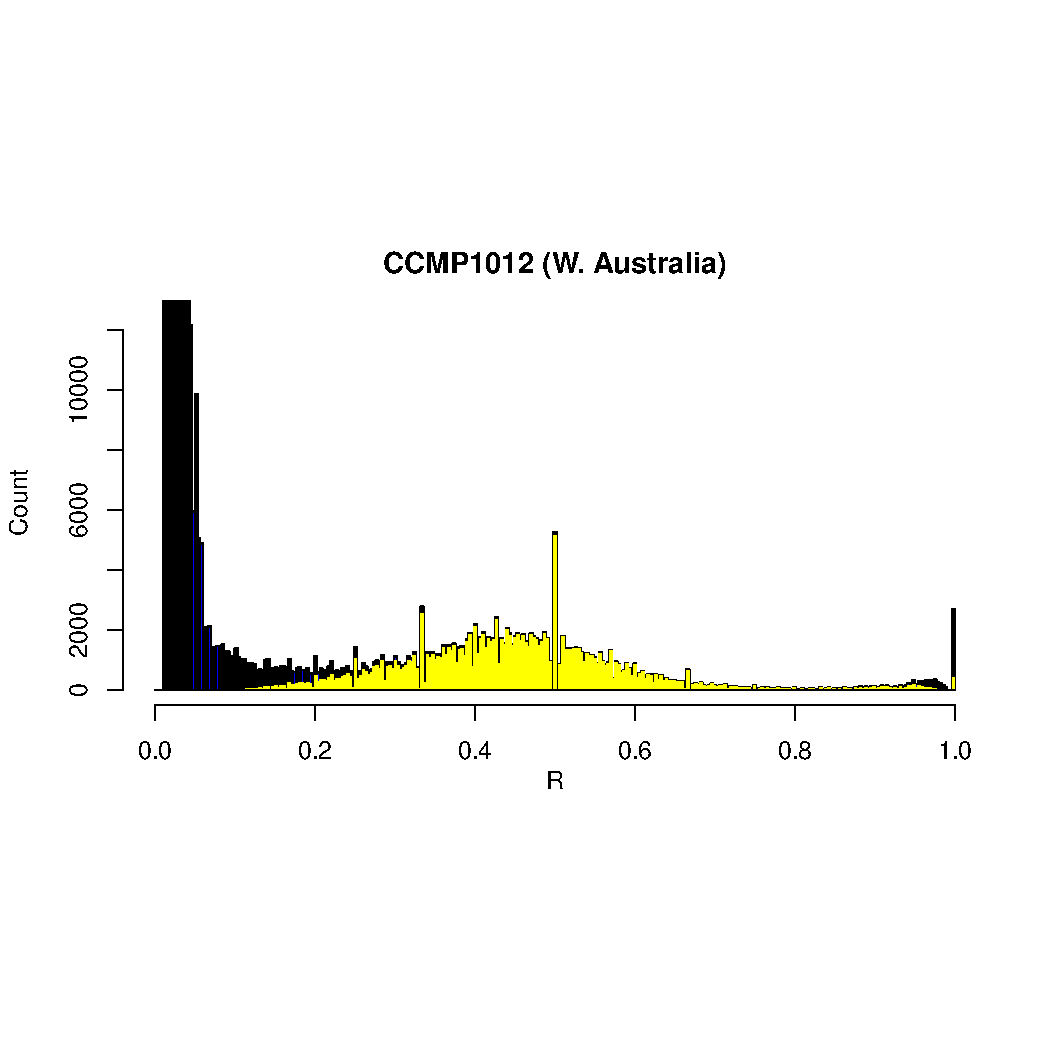
\includegraphics[width=\maxwidth]{FigS7-hwe-histo-figs-knitr/unnamed-chunk-10-31} 
\begin{kframe}\begin{verbatim}
#      [,1]     [,2]     [,3]   [,4]    [,5]  [,6]    [,7]    [,8]     [,9]     [,10]    [,11] 
# [1,] "blue"   "nm3"    "nm3x" "nm3hi" "red" "black" "green" "orange" "ornghi" "nzgrey" "grey"
# [2,] "203028" "181216" NA     "0"     NA    NA      NA      NA       NA       NA       NA
# 
# homnr:het ratios vs mod.humpth lo x hi, full-qfiltered :
#       hi
# lo          0.7     0.75     0.76     0.77     0.78     0.79      0.8     0.85      0.9
#   0.1  14.37715 16.72467 17.00154 17.39350 17.74814 18.06403 18.44932 19.86433 22.57843
#   0.15 13.35574 15.54733 15.80580 16.17172 16.50281 16.79771 17.15741 18.47843 21.01225
#   0.16 13.18433 15.34976 15.60515 15.96670 16.29383 16.58521 16.94062 18.24586 20.74943
#   0.17 13.03492 15.17754 15.43024 15.78798 16.11167 16.39998 16.75164 18.04314 20.52033
#   0.18 12.86467 14.98130 15.23093 15.58433 15.90410 16.18891 16.53631 17.81214 20.25928
#   0.19 12.71782 14.81202 15.05901 15.40867 15.72505 16.00684 16.35056 17.61287 20.03410
#   0.2  12.51100 14.57363 14.81689 15.16128 15.47289 15.75043 16.08897 17.33225 19.71697
#   0.25 11.65637 13.58853 13.81641 14.13901 14.43091 14.69090 15.00802 16.17266 18.40654
# 
# 
# 1013 coverage summary for retained sites:
#    Min. 1st Qu.  Median    Mean 3rd Qu.    Max. 
#   14.00   31.00   41.00   42.11   52.00   77.00 
# FigS7-hwe-histo-figs-mine/S7-full-qfiltered-1013chronly.pdf :
#   based on 27774773 positions with coverage in [ 13.57311 , 77.23415 ]
\end{verbatim}
\end{kframe}
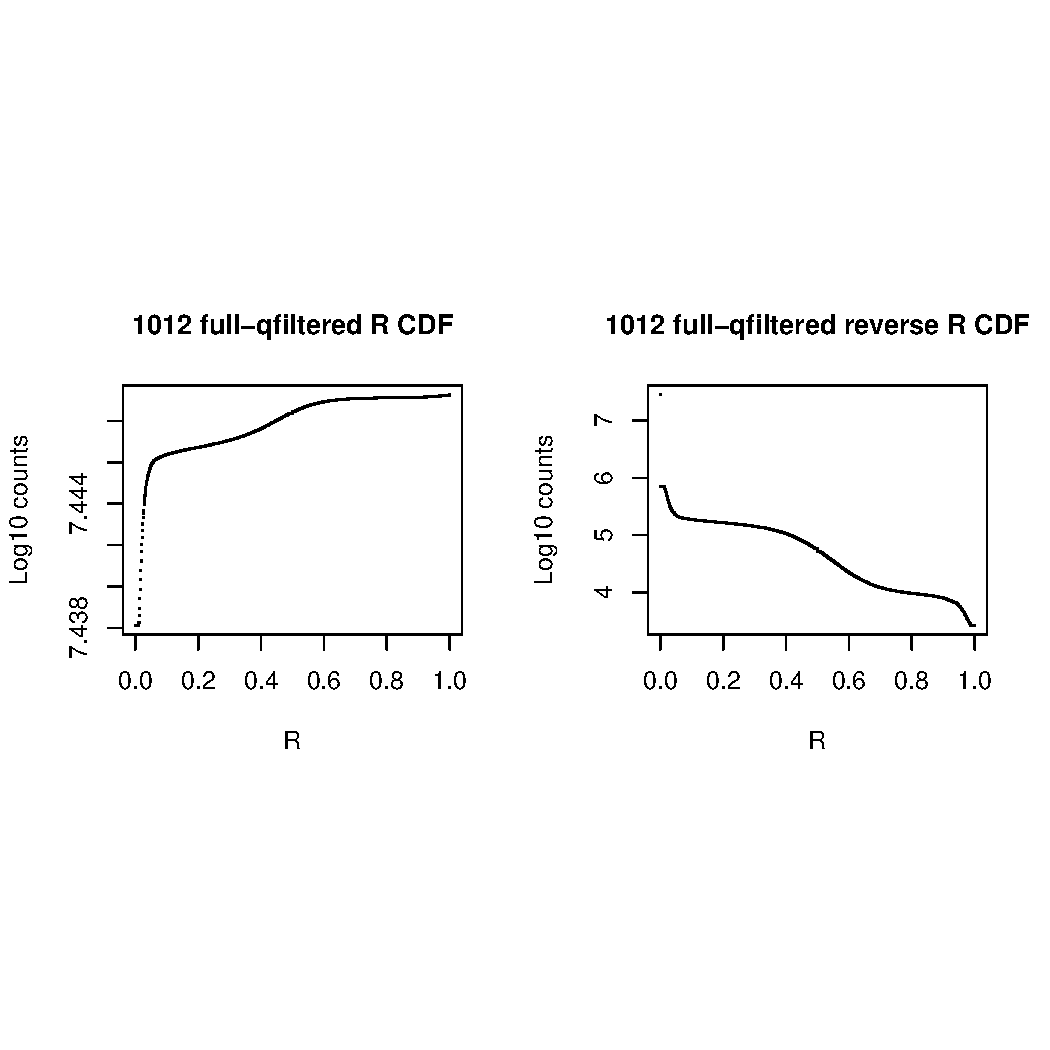
\includegraphics[width=\maxwidth]{FigS7-hwe-histo-figs-knitr/unnamed-chunk-10-32} 
\begin{kframe}\begin{verbatim}
#      [,1]     [,2]     [,3]     [,4]     [,5]  [,6]    [,7]    [,8]     [,9]     [,10]    [,11] 
# [1,] "blue"   "nm3"    "nm3x"   "nm3hi"  "red" "black" "green" "orange" "ornghi" "nzgrey" "grey"
# [2,] "343032" "194277" "388554" "101630" NA    NA      NA      "388554" "101630" NA       NA    
# FigS7-hwe-histo-figs-mine/S7-full-qfiltered-1013chronly.pdf written; 301-bin histo follows:
\end{verbatim}
\end{kframe}
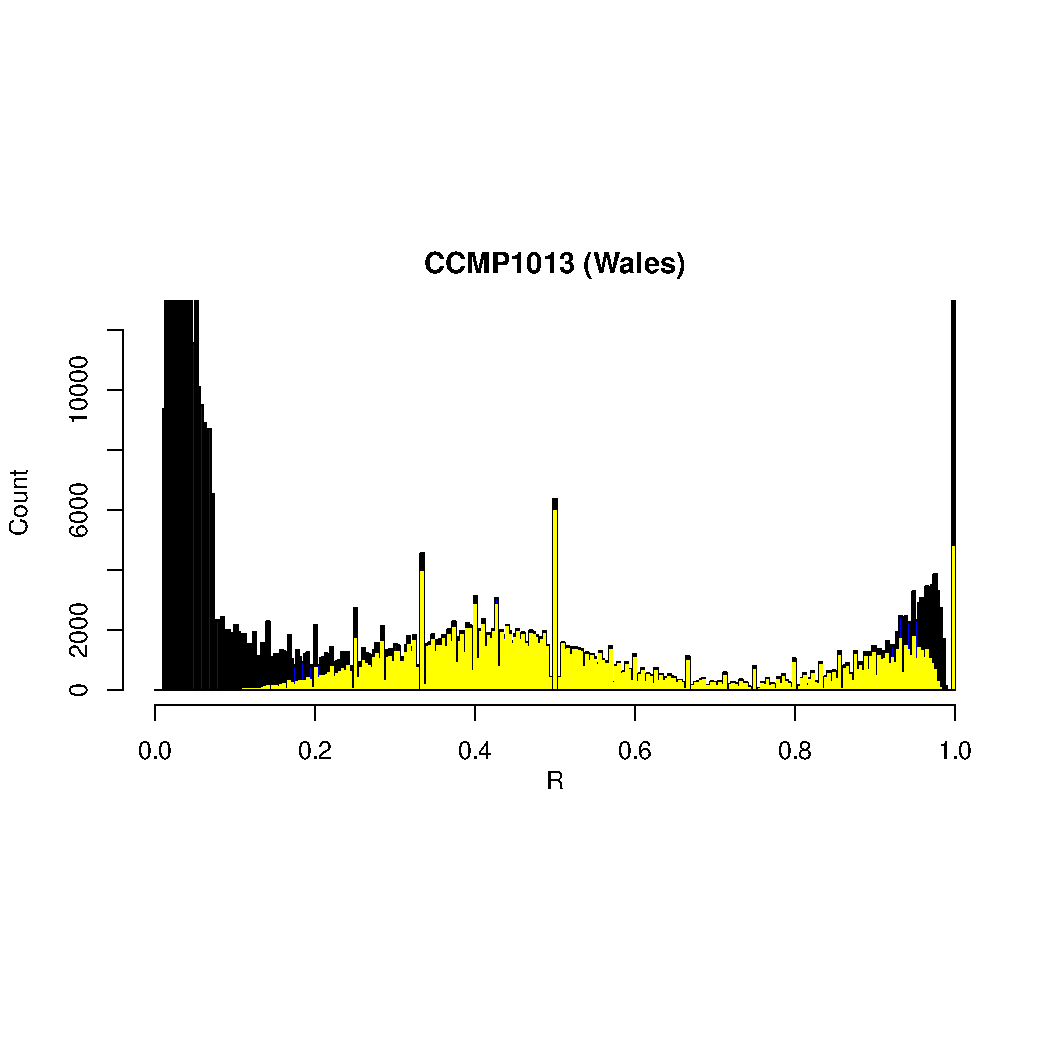
\includegraphics[width=\maxwidth]{FigS7-hwe-histo-figs-knitr/unnamed-chunk-10-33} 
\begin{kframe}\begin{verbatim}
#      [,1]     [,2]     [,3]   [,4]    [,5]  [,6]    [,7]    [,8]     [,9]     [,10]    [,11] 
# [1,] "blue"   "nm3"    "nm3x" "nm3hi" "red" "black" "green" "orange" "ornghi" "nzgrey" "grey"
# [2,] "343032" "224543" NA     "0"     NA    NA      NA      NA       NA       NA       NA
# 
# homnr:het ratios vs mod.humpth lo x hi, full-qfiltered :
#       hi
# lo          0.7     0.75     0.76     0.77     0.78     0.79      0.8     0.85      0.9
#   0.1  2.051954 2.166533 2.176196 2.199631 2.221735 2.256683 2.302579 2.509275 3.064857
#   0.15 1.848700 1.955648 1.964668 1.986542 2.007174 2.039794 2.082633 2.275564 2.794145
#   0.16 1.817728 1.923514 1.932436 1.954072 1.974479 2.006745 2.049119 2.239952 2.752895
#   0.17 1.790490 1.895253 1.904088 1.925515 1.945726 1.977679 2.019643 2.208632 2.716617
#   0.18 1.759649 1.863254 1.871992 1.893182 1.913169 1.944769 1.986270 2.173169 2.675540
#   0.19 1.731340 1.833882 1.842531 1.863503 1.883285 1.914562 1.955636 2.140618 2.637836
#   0.2  1.690091 1.791085 1.799603 1.820259 1.839742 1.870546 1.911000 2.093189 2.582897
#   0.25 1.534639 1.629797 1.637822 1.657285 1.675642 1.704666 1.742782 1.914443 2.375852
# 
# 
# 1014 coverage summary for retained sites:
#    Min. 1st Qu.  Median    Mean 3rd Qu.    Max. 
#    3.00    8.00   11.00   11.92   16.00   24.00 
# FigS7-hwe-histo-figs-mine/S7-full-qfiltered-1014chronly.pdf :
#   based on 27380065 positions with coverage in [ 2.498888 , 24.95332 ]
\end{verbatim}
\end{kframe}
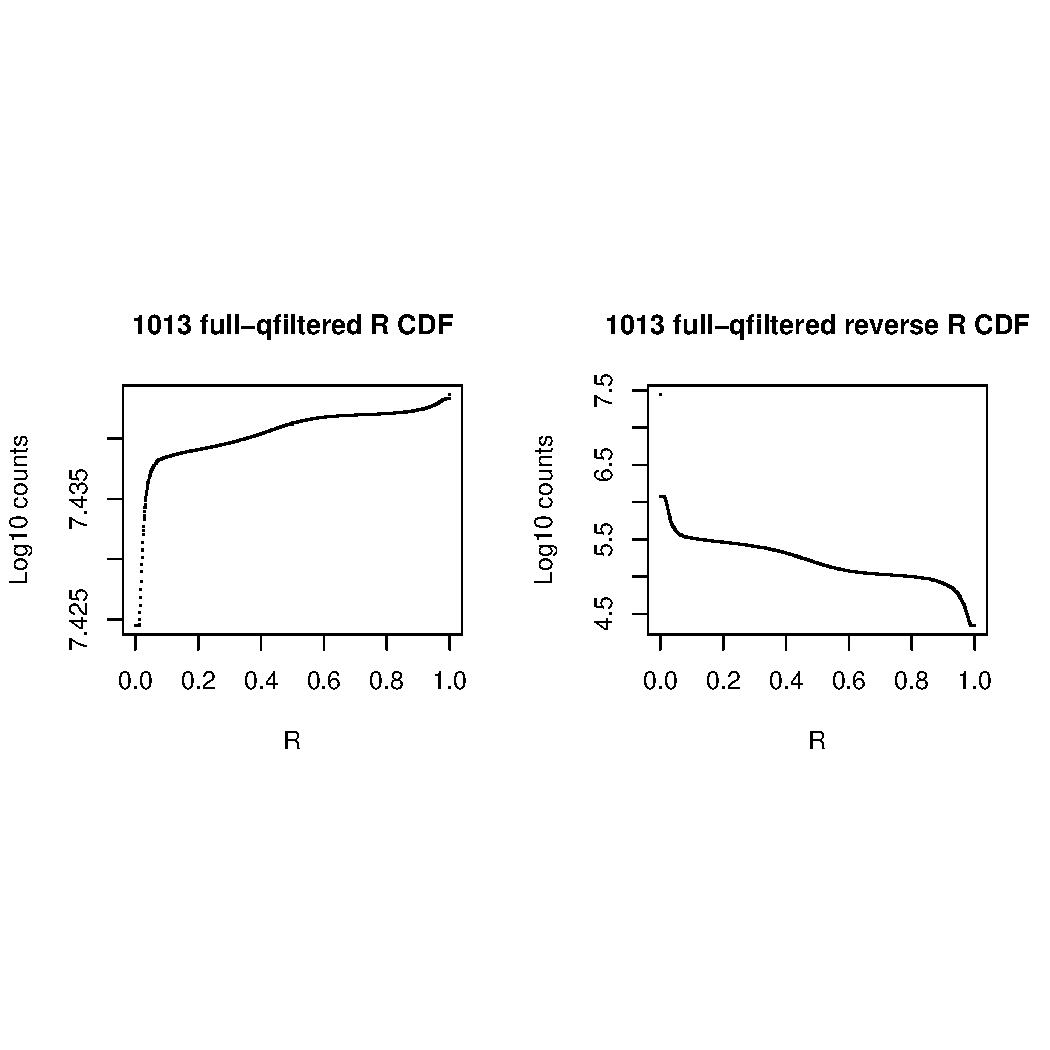
\includegraphics[width=\maxwidth]{FigS7-hwe-histo-figs-knitr/unnamed-chunk-10-34} 
\begin{kframe}\begin{verbatim}
#      [,1]     [,2]    [,3]     [,4]    [,5]  [,6]    [,7]    [,8]     [,9]     [,10]    [,11] 
# [1,] "blue"   "nm3"   "nm3x"   "nm3hi" "red" "black" "green" "orange" "ornghi" "nzgrey" "grey"
# [2,] "110916" "98608" "197216" "7160"  NA    NA      NA      "197216" "7160"   NA       NA    
# FigS7-hwe-histo-figs-mine/S7-full-qfiltered-1014chronly.pdf written; 301-bin histo follows:
\end{verbatim}
\end{kframe}
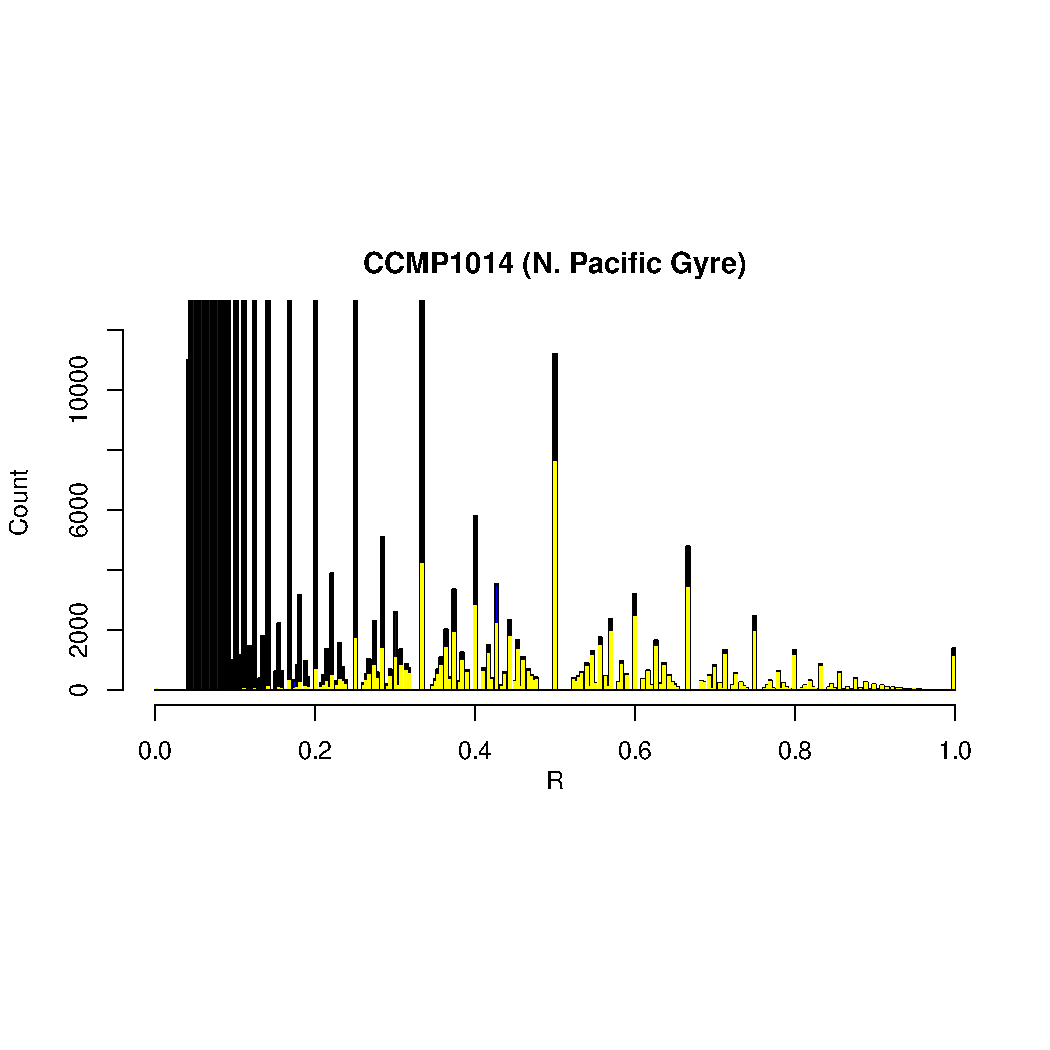
\includegraphics[width=\maxwidth]{FigS7-hwe-histo-figs-knitr/unnamed-chunk-10-35} 
\begin{kframe}\begin{verbatim}
#      [,1]     [,2]    [,3]   [,4]    [,5]  [,6]    [,7]    [,8]     [,9]     [,10]    [,11] 
# [1,] "blue"   "nm3"   "nm3x" "nm3hi" "red" "black" "green" "orange" "ornghi" "nzgrey" "grey"
# [2,] "110916" "86872" NA     "0"     NA    NA      NA      NA       NA       NA       NA
# 
# homnr:het ratios vs mod.humpth lo x hi, full-qfiltered :
#       hi
# lo          0.7     0.75     0.76     0.77     0.78     0.79      0.8     0.85       0.9
#   0.1  23.65374 39.01957 39.01957 41.74126 45.84039 48.21041 60.61859 91.13350 167.07022
#   0.15 15.04792 25.05004 25.05004 26.82168 29.48994 31.03266 39.10955 58.97270 108.40239
#   0.16 14.82263 24.68434 24.68434 26.43110 29.06190 30.58297 38.54647 58.13077 106.86653
#   0.17 12.48952 20.89707 20.89707 22.38627 24.62915 25.92593 32.71517 49.41168  90.96116
#   0.18 12.40485 20.75963 20.75963 22.23949 24.46829 25.75693 32.50356 49.09528  90.38396
#   0.19 12.08554 20.24131 20.24131 21.68592 23.86162 25.11957 31.70550 47.90199  88.20717
#   0.2  10.00986 16.87193 16.87193 18.08739 19.91797 20.97638 26.51762 40.14496  74.05677
#   0.25  7.60114 12.96194 12.96194 13.91147 15.34157 16.16842 20.49735 31.14333  57.63596
# 
# 
# 1015 coverage summary for retained sites:
#    Min. 1st Qu.  Median    Mean 3rd Qu.    Max. 
#   17.00   36.00   45.00   46.15   56.00   80.00 
# FigS7-hwe-histo-figs-mine/S7-full-qfiltered-1015chronly.pdf :
#   based on 28260470 positions with coverage in [ 16.94128 , 80.63472 ]
\end{verbatim}
\end{kframe}
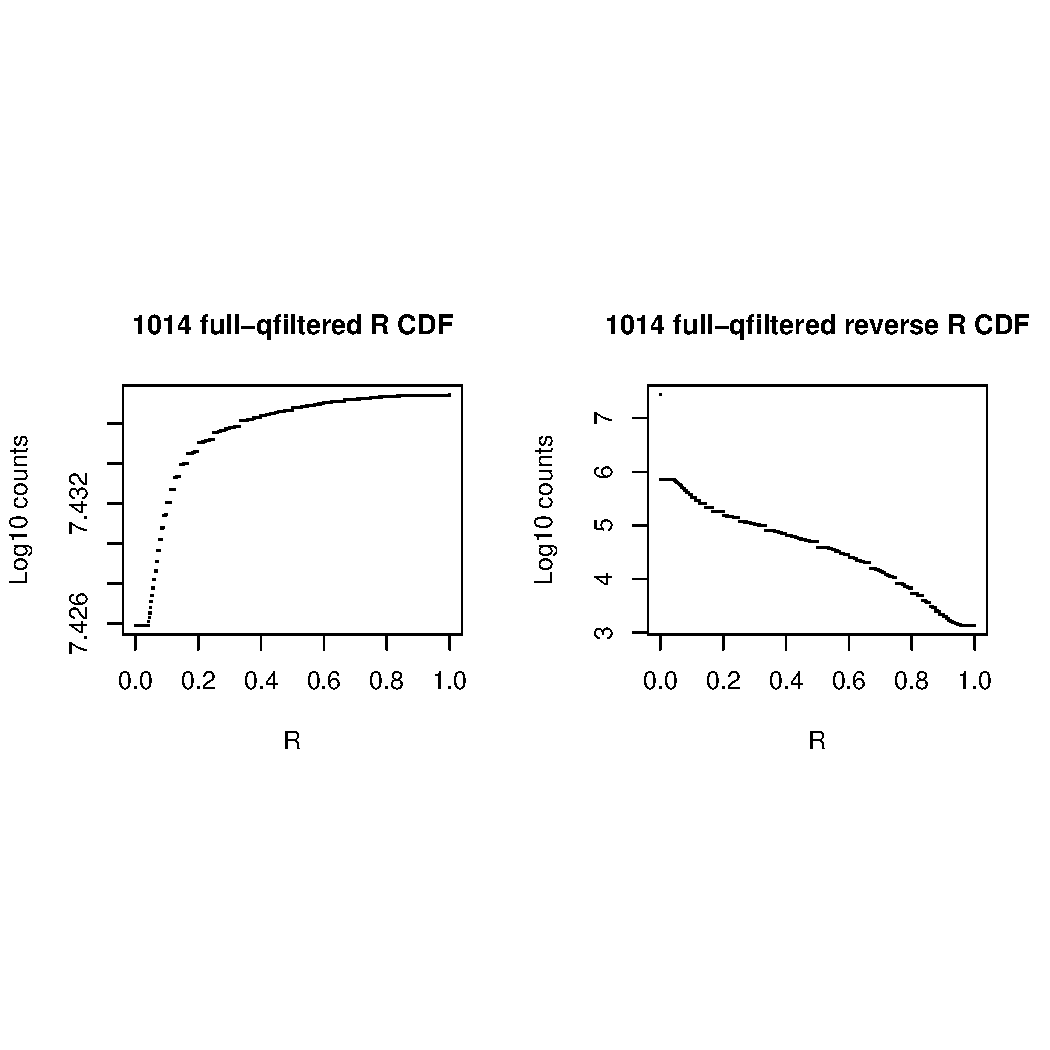
\includegraphics[width=\maxwidth]{FigS7-hwe-histo-figs-knitr/unnamed-chunk-10-36} 
\begin{kframe}\begin{verbatim}
#      [,1]     [,2]     [,3]     [,4]    [,5]  [,6]    [,7]    [,8]     [,9]     [,10]    [,11] 
# [1,] "blue"   "nm3"    "nm3x"   "nm3hi" "red" "black" "green" "orange" "ornghi" "nzgrey" "grey"
# [2,] "211232" "171287" "342574" "4220"  NA    NA      NA      "342574" "4220"   NA       NA    
# FigS7-hwe-histo-figs-mine/S7-full-qfiltered-1015chronly.pdf written; 301-bin histo follows:
\end{verbatim}
\end{kframe}
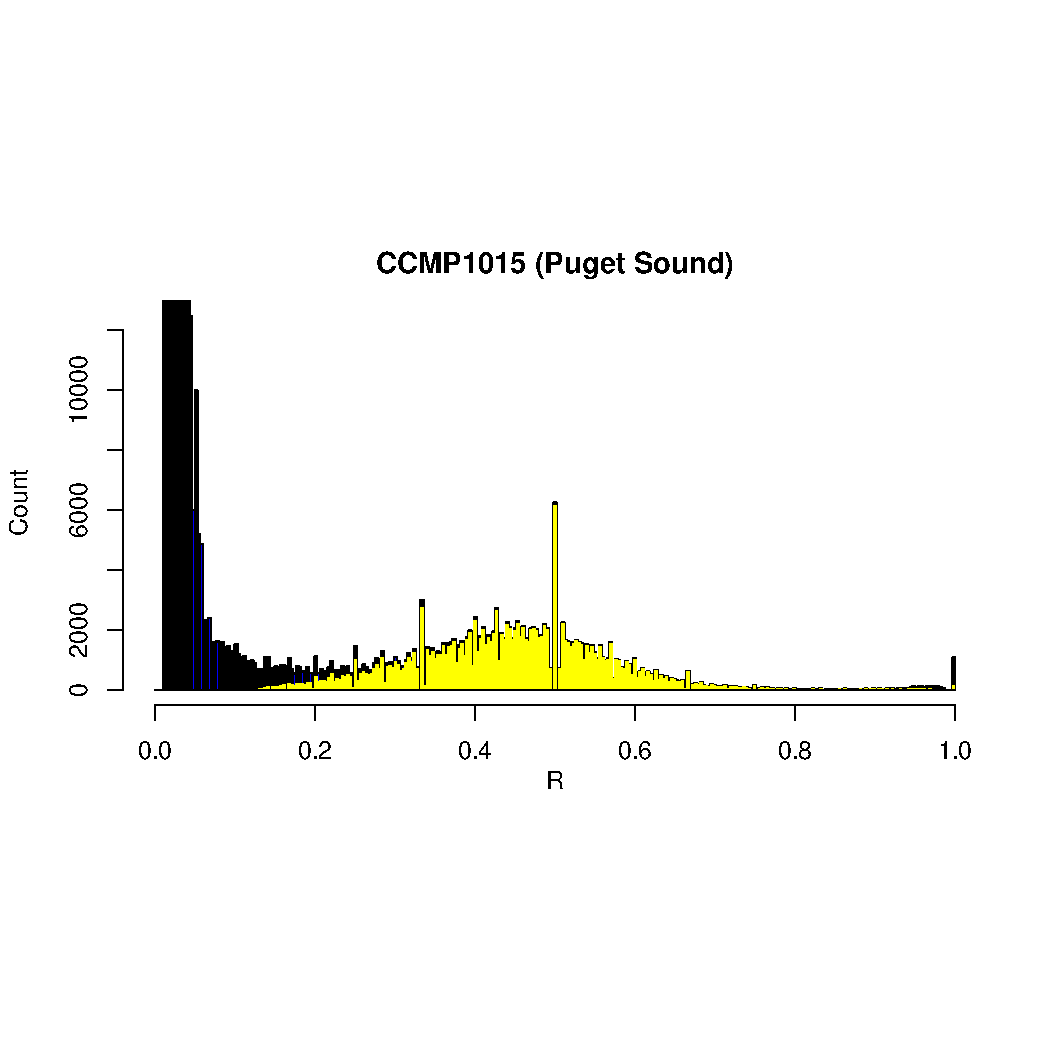
\includegraphics[width=\maxwidth]{FigS7-hwe-histo-figs-knitr/unnamed-chunk-10-37} 
\begin{kframe}\begin{verbatim}
#      [,1]     [,2]     [,3]   [,4]    [,5]  [,6]    [,7]    [,8]     [,9]     [,10]    [,11] 
# [1,] "blue"   "nm3"    "nm3x" "nm3hi" "red" "black" "green" "orange" "ornghi" "nzgrey" "grey"
# [2,] "211232" "194644" NA     "0"     NA    NA      NA      NA       NA       NA       NA
# 
# homnr:het ratios vs mod.humpth lo x hi, full-qfiltered :
#       hi
# lo          0.7     0.75     0.76     0.77     0.78     0.79      0.8     0.85      0.9
#   0.1  30.30116 40.75723 41.99162 43.67698 45.15846 46.74155 48.26213 53.83427 61.80406
#   0.15 28.21217 37.97043 39.12244 40.69532 42.07793 43.55537 44.97447 50.17473 57.61263
#   0.16 27.87119 37.51553 38.65409 40.20862 41.57508 43.03528 44.43782 49.57738 56.92846
#   0.17 27.57324 37.11806 38.24487 39.78336 41.13572 42.58084 43.96891 49.05543 56.33065
#   0.18 27.23177 36.66252 37.77587 39.29597 40.63216 42.06002 43.43150 48.45723 55.64550
#   0.19 26.95262 36.29012 37.39246 38.89752 40.22051 41.63425 42.99216 47.96820 55.08540
#   0.2  26.54128 35.74138 36.82749 38.31041 39.61393 41.00686 42.34479 47.24761 54.26007
#   0.25 24.89062 33.53932 34.56034 35.95438 37.17977 38.48922 39.74697 44.35594 50.94811
# 
# 
# 3367 coverage summary for retained sites:
#    Min. 1st Qu.  Median    Mean 3rd Qu.    Max. 
#   16.00   34.00   43.00   43.42   53.00   74.00 
# FigS7-hwe-histo-figs-mine/S7-full-qfiltered-3367chronly.pdf :
#   based on 28281913 positions with coverage in [ 15.4759 , 74.13251 ]
\end{verbatim}
\end{kframe}
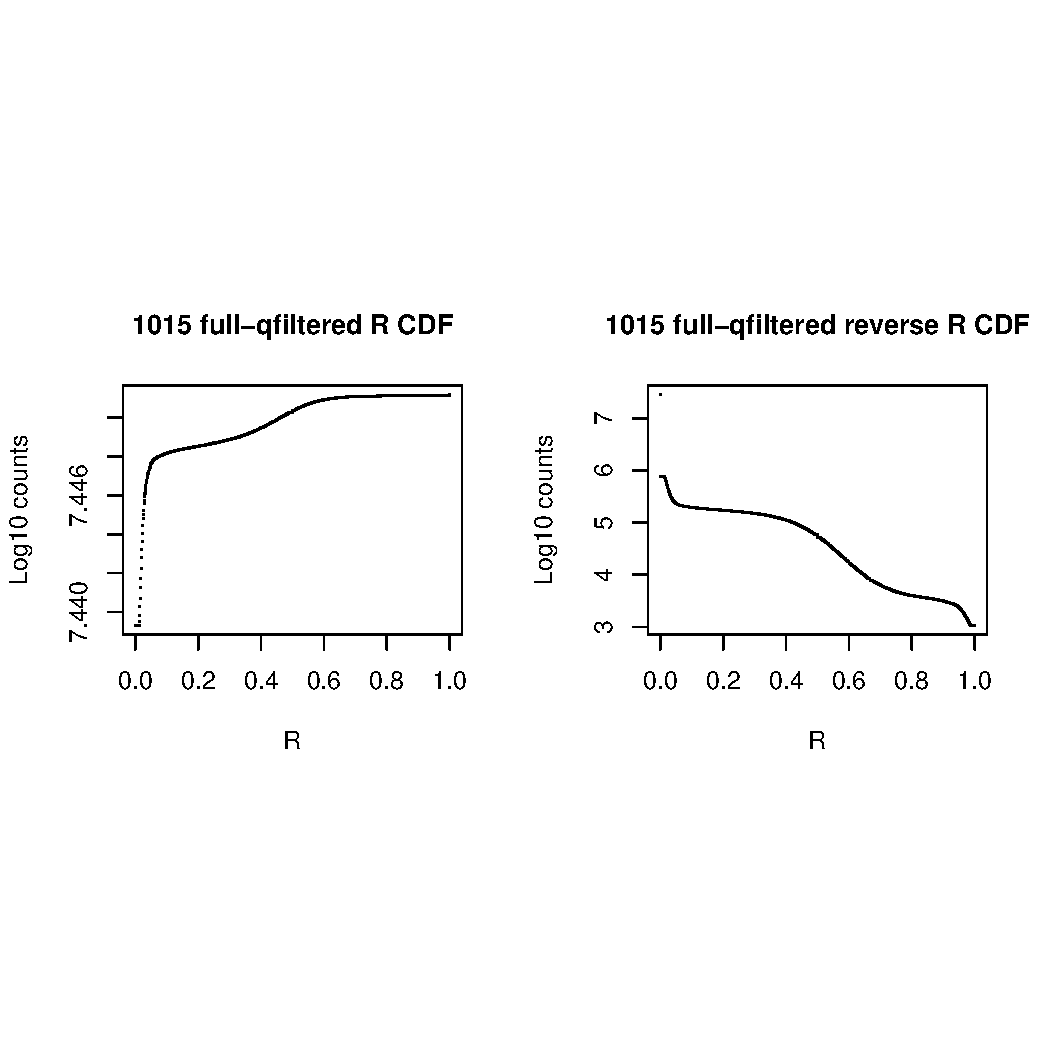
\includegraphics[width=\maxwidth]{FigS7-hwe-histo-figs-knitr/unnamed-chunk-10-38} 
\begin{kframe}\begin{verbatim}
#      [,1]     [,2]     [,3]     [,4]     [,5]  [,6]    [,7]    [,8]     [,9]     [,10]    [,11] 
# [1,] "blue"   "nm3"    "nm3x"   "nm3hi"  "red" "black" "green" "orange" "ornghi" "nzgrey" "grey"
# [2,] "323459" "164201" "328402" "117569" NA    NA      NA      "328402" "117569" NA       NA    
# FigS7-hwe-histo-figs-mine/S7-full-qfiltered-3367chronly.pdf written; 301-bin histo follows:
\end{verbatim}
\end{kframe}
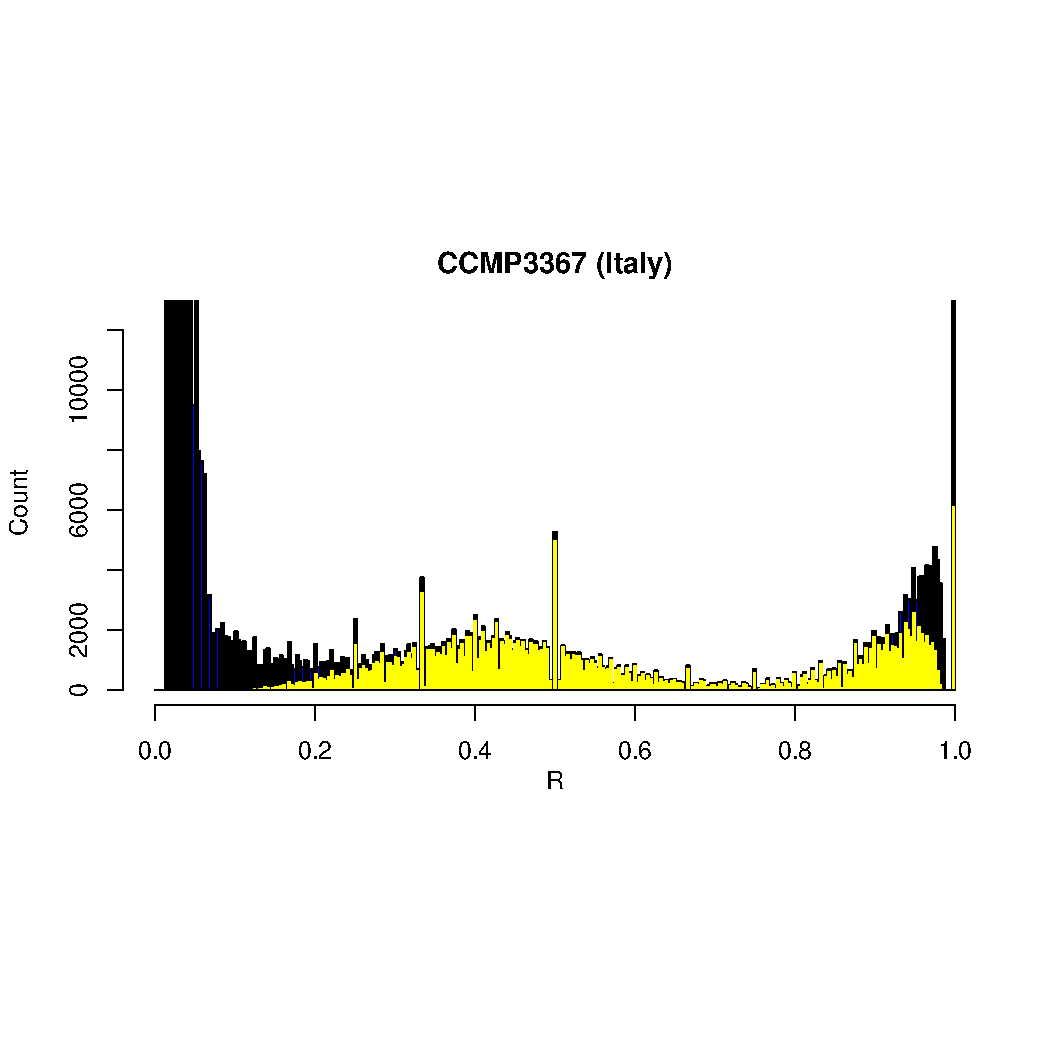
\includegraphics[width=\maxwidth]{FigS7-hwe-histo-figs-knitr/unnamed-chunk-10-39} 
\begin{kframe}\begin{verbatim}
#      [,1]     [,2]     [,3]   [,4]    [,5]  [,6]    [,7]    [,8]     [,9]     [,10]    [,11] 
# [1,] "blue"   "nm3"    "nm3x" "nm3hi" "red" "black" "green" "orange" "ornghi" "nzgrey" "grey"
# [2,] "323459" "191716" NA     "0"     NA    NA      NA      NA       NA       NA       NA
# 
# homnr:het ratios vs mod.humpth lo x hi, full-qfiltered :
#       hi
# lo          0.7     0.75     0.76     0.77     0.78     0.79      0.8     0.85      0.9
#   0.1  1.512561 1.578044 1.583807 1.599163 1.613325 1.629148 1.650408 1.804258 2.236845
#   0.15 1.372583 1.434417 1.439859 1.454360 1.467733 1.482674 1.502750 1.648029 2.056516
#   0.16 1.349635 1.410871 1.416260 1.430621 1.443865 1.458661 1.478543 1.622416 2.026952
#   0.17 1.328967 1.389664 1.395006 1.409240 1.422367 1.437034 1.456741 1.599349 2.000326
#   0.18 1.306124 1.366227 1.371516 1.385611 1.398609 1.413132 1.432645 1.573855 1.970900
#   0.19 1.285211 1.344768 1.350010 1.363977 1.376857 1.391248 1.410585 1.550514 1.943958
#   0.2  1.258038 1.316887 1.322066 1.335867 1.348594 1.362814 1.381920 1.520185 1.908951
#   0.25 1.143100 1.198953 1.203869 1.216967 1.229047 1.242543 1.260677 1.391904 1.760881
# 
# 
# 1335 coverage summary for retained sites:
#    Min. 1st Qu.  Median    Mean 3rd Qu.    Max. 
#   38.00   63.00   80.00   80.16   97.00  126.00 
# FigS7-hwe-histo-figs-mine/S7-full-qfiltered-1335chronly.pdf :
#   based on 26550021 positions with coverage in [ 37.70838 , 126.0564 ]
\end{verbatim}
\end{kframe}
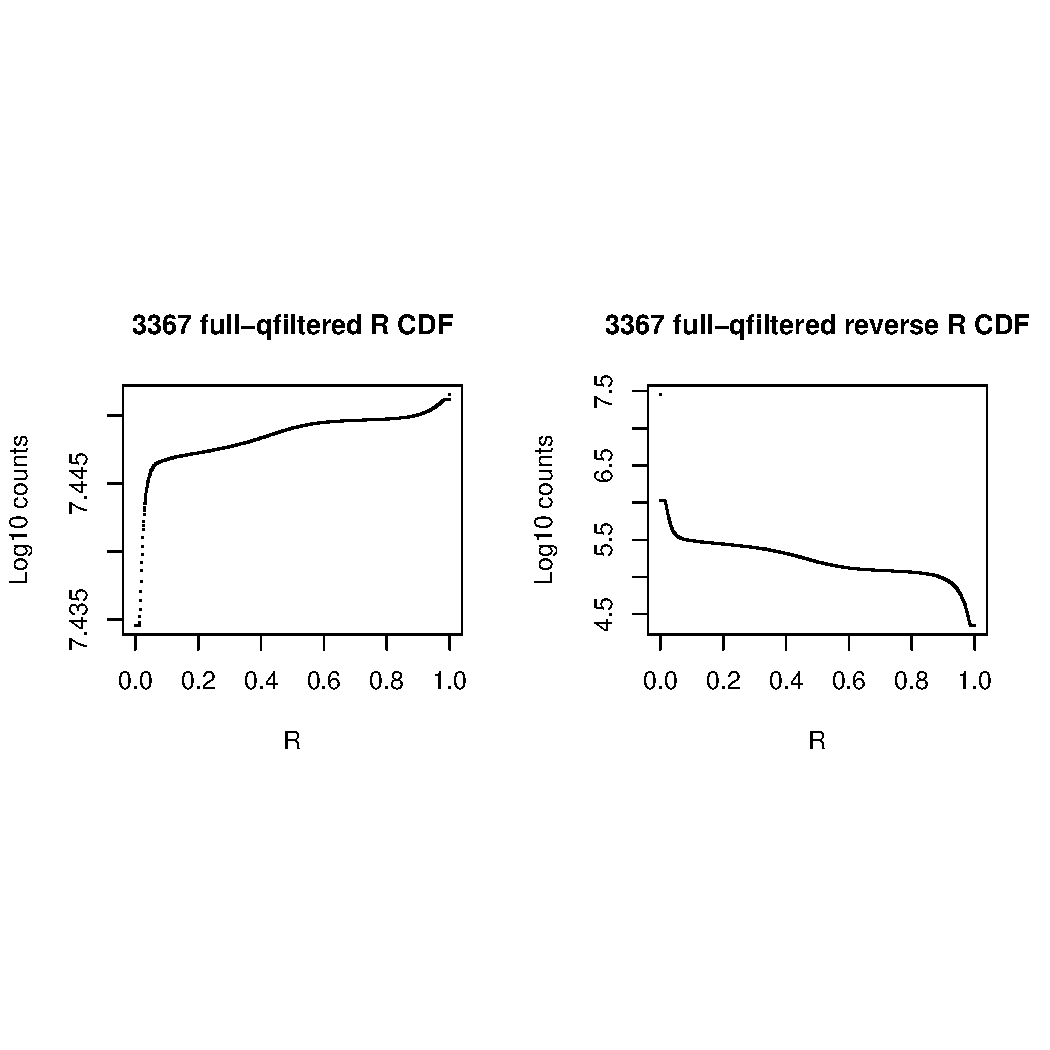
\includegraphics[width=\maxwidth]{FigS7-hwe-histo-figs-knitr/unnamed-chunk-10-40} 
\begin{kframe}\begin{verbatim}
#      [,1]     [,2]     [,3]     [,4]    [,5]  [,6]    [,7]    [,8]     [,9]     [,10]    [,11] 
# [1,] "blue"   "nm3"    "nm3x"   "nm3hi" "red" "black" "green" "orange" "ornghi" "nzgrey" "grey"
# [2,] "187629" "140476" "280952" "525"   NA    NA      NA      "280952" "525"    NA       NA    
# FigS7-hwe-histo-figs-mine/S7-full-qfiltered-1335chronly.pdf written; 301-bin histo follows:
\end{verbatim}
\end{kframe}
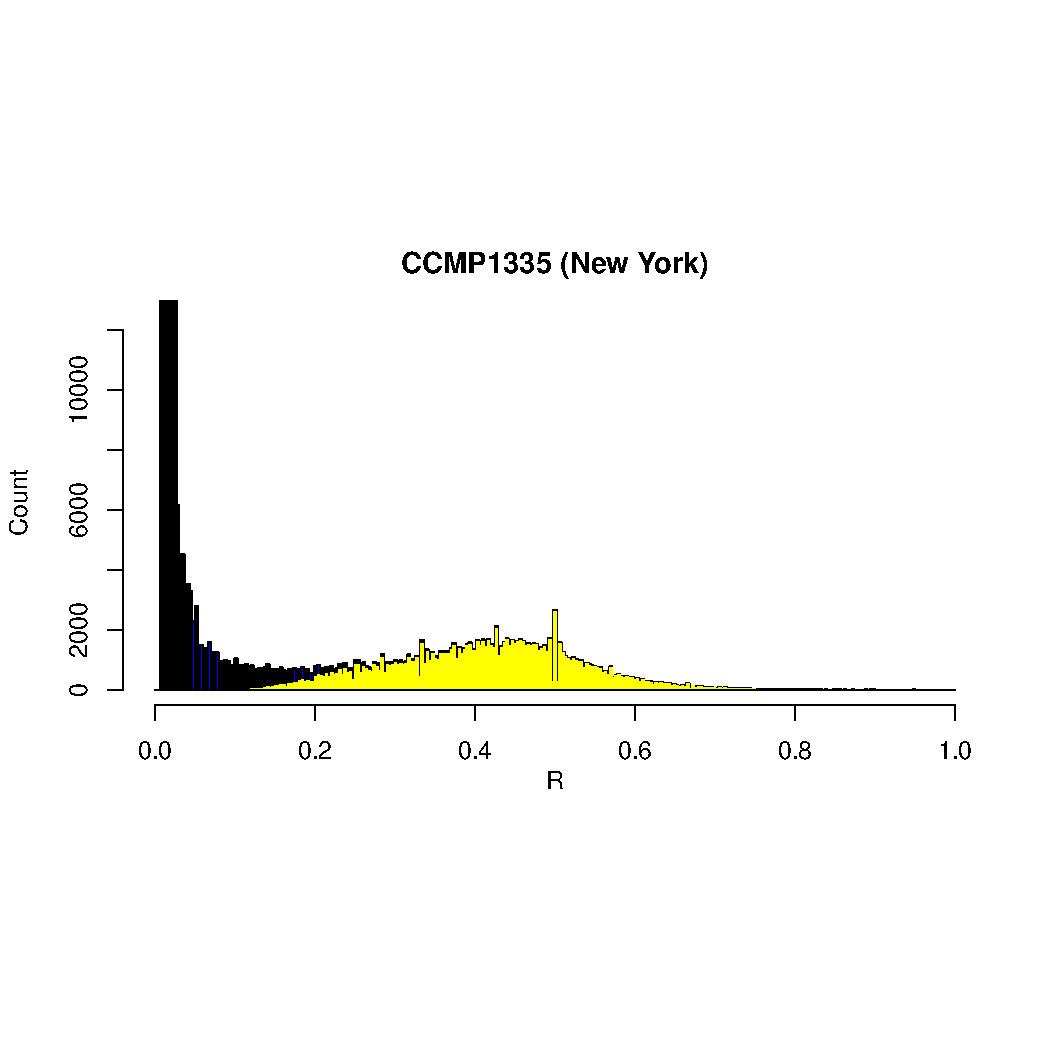
\includegraphics[width=\maxwidth]{FigS7-hwe-histo-figs-knitr/unnamed-chunk-10-41} 
\begin{kframe}\begin{verbatim}
#      [,1]     [,2]     [,3]   [,4]    [,5]  [,6]    [,7]    [,8]     [,9]     [,10]    [,11] 
# [1,] "blue"   "nm3"    "nm3x" "nm3hi" "red" "black" "green" "orange" "ornghi" "nzgrey" "grey"
# [2,] "187629" "180473" NA     "0"     NA    NA      NA      NA       NA       NA       NA
# 
# homnr:het ratios vs mod.humpth lo x hi, full-qfiltered :
#       hi
# lo          0.7     0.75     0.76     0.77     0.78     0.79      0.8     0.85      0.9
#   0.1  97.65646 208.4814 230.9369 264.4605 298.7135 336.4979 405.0386 751.1381 1610.724
#   0.15 90.82948 193.9854 214.8869 246.0908 277.9734 313.1432 376.9409 699.0905 1499.194
#   0.16 89.54216 191.2520 211.8605 242.6269 274.0626 308.7393 371.6427 689.2762 1478.163
#   0.17 88.40537 188.8382 209.1880 239.5681 270.6091 304.8504 366.9640 680.6095 1459.592
#   0.18 87.10806 186.0836 206.1380 236.0773 266.6679 300.4124 361.6247 670.7190 1438.398
#   0.19 85.92755 183.5769 203.3627 232.9008 263.0816 296.3739 356.7661 661.7190 1419.112
#   0.2  84.46284 180.4668 199.9192 228.9597 258.6319 291.3632 350.7378 650.5524 1395.184
#   0.25 77.46221 165.6021 183.4611 210.1227 237.3643 267.4145 321.9254 597.1810 1280.816
# 
# 
# 
# ***
# *
# * Processing Chr1-qfiltered 
# *
# ***
# Chr1-qfiltered coverage stats:
#                   1007     1012     1013      1014     1015     3367     1335
# cov.means.all 27.58495 49.25573 43.22936 12.431987 46.98747 43.44037 78.77898
# cov.sigs.all  11.57294 20.93111 21.50588  7.358896 19.36047 18.78854 29.76521
# cov.means     27.58495 49.25573 43.22936 12.431987 46.98747 43.44037 78.77898
# cov.sigs      11.57294 20.93111 21.50588  7.358896 19.36047 18.78854 29.76521
# cov.min       16.01202 28.32462 21.72348  5.073091 27.62700 24.65183 49.01378
# 
# 
# 1007 coverage summary for retained sites:
#    Min. 1st Qu.  Median    Mean 3rd Qu.    Max. 
#   17.00   22.00   27.00   27.06   32.00   39.00 
# FigS7-hwe-histo-figs-mine/S7-Chr1-qfiltered-1007.pdf :
#   based on 2274114 positions with coverage in [ 16.01202 , 39.15789 ]
\end{verbatim}
\end{kframe}
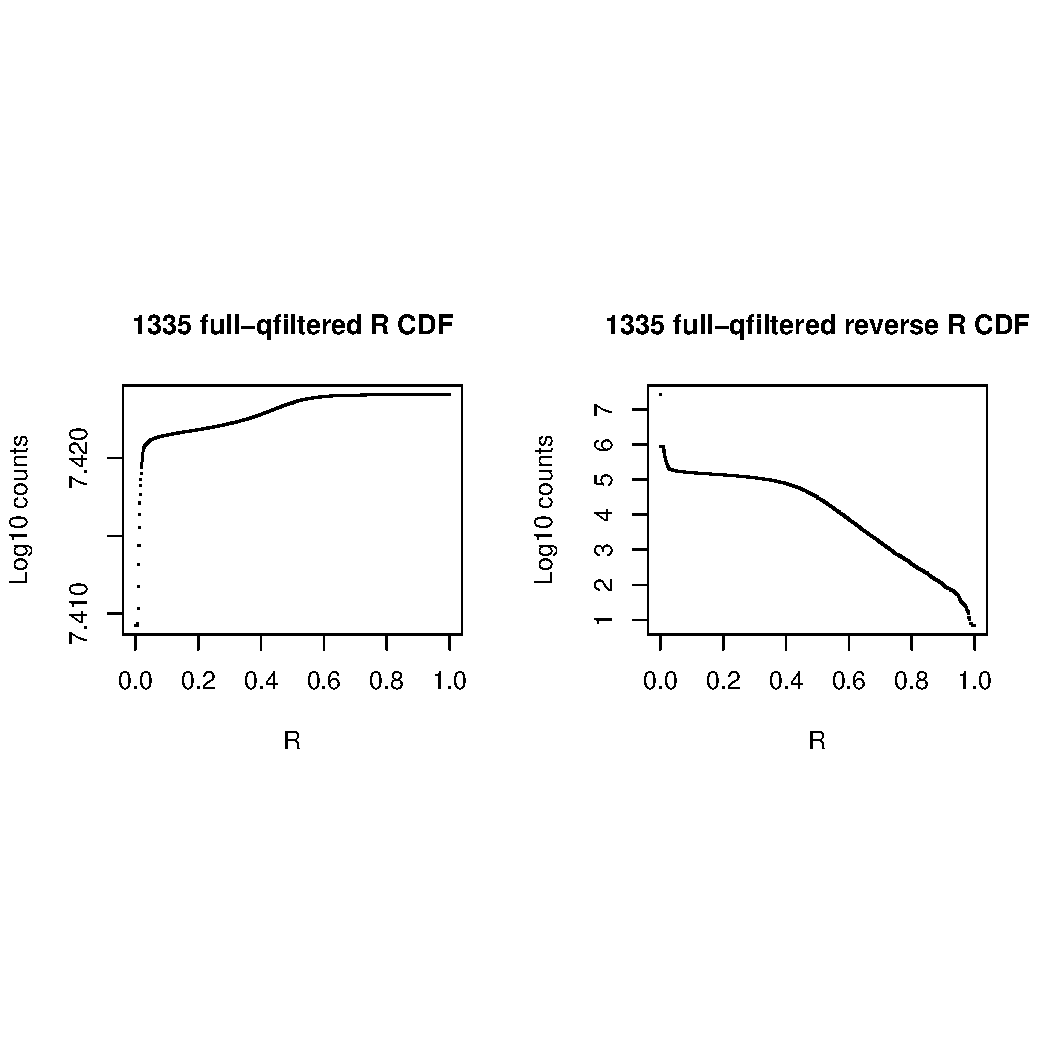
\includegraphics[width=\maxwidth]{FigS7-hwe-histo-figs-knitr/unnamed-chunk-10-42} 
\begin{kframe}\begin{verbatim}
#      [,1]    [,2]    [,3]    [,4]    [,5]  [,6]    [,7]    [,8]     [,9]     [,10]    [,11] 
# [1,] "blue"  "nm3"   "nm3x"  "nm3hi" "red" "black" "green" "orange" "ornghi" "nzgrey" "grey"
# [2,] "14568" "13279" "26558" "84"    NA    NA      NA      "26558"  "84"     NA       NA    
# FigS7-hwe-histo-figs-mine/S7-Chr1-qfiltered-1007.pdf written; 301-bin histo follows:
\end{verbatim}
\end{kframe}
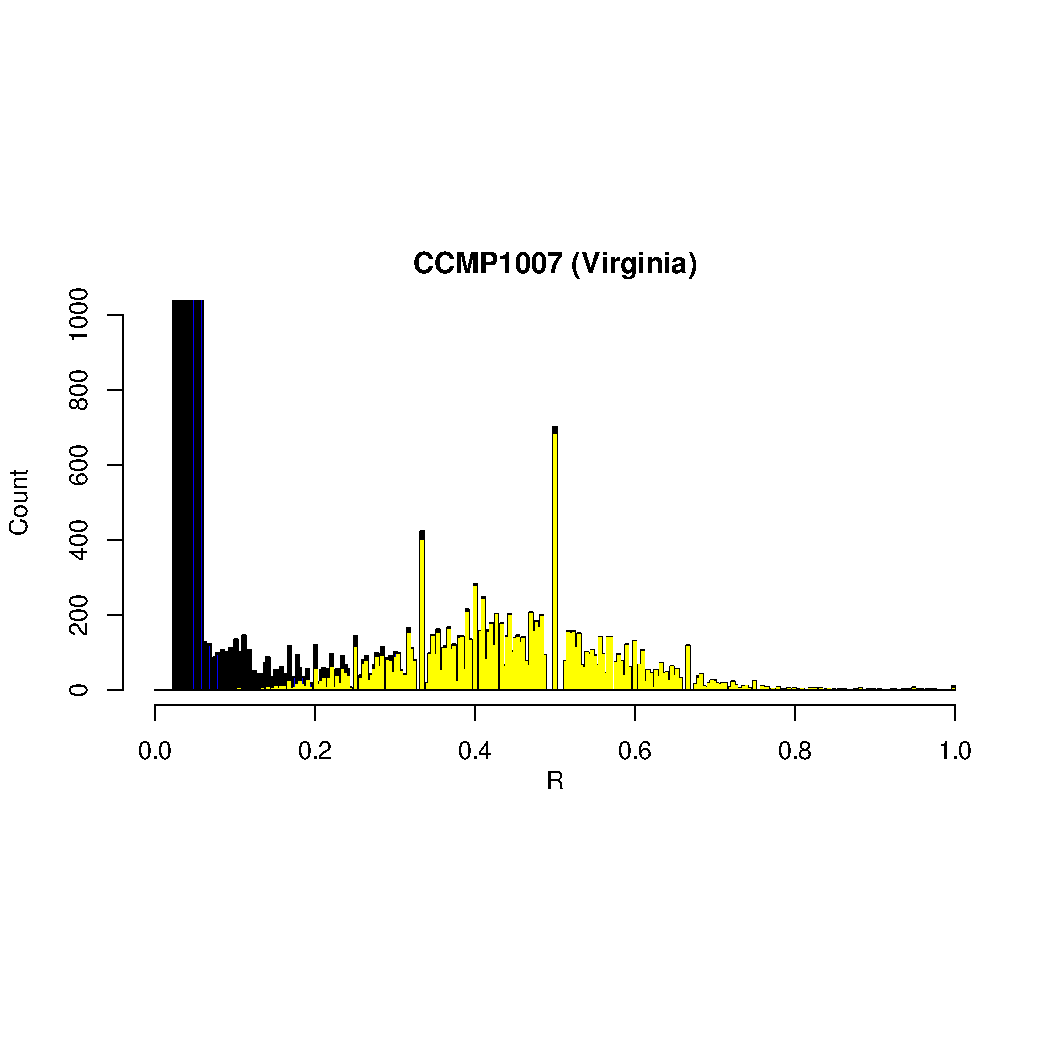
\includegraphics[width=\maxwidth]{FigS7-hwe-histo-figs-knitr/unnamed-chunk-10-43} 
\begin{kframe}\begin{verbatim}
#      [,1]    [,2]    [,3]   [,4]    [,5]  [,6]    [,7]    [,8]     [,9]     [,10]    [,11] 
# [1,] "blue"  "nm3"   "nm3x" "nm3hi" "red" "black" "green" "orange" "ornghi" "nzgrey" "grey"
# [2,] "14568" "13220" NA     "0"     NA    NA      NA      NA       NA       NA       NA
# 
# homnr:het ratios vs mod.humpth lo x hi, Chr1-qfiltered :
#       hi
# lo          0.7      0.75     0.76     0.77     0.78     0.79      0.8     0.85      0.9
#   0.1  49.61379 119.31148 130.0536 151.8958 173.7381 184.7975 208.6857 332.5909 443.7879
#   0.15 46.55862 112.04918 122.1429 142.6667 163.1905 173.5823 196.0286 312.4545 416.9394
#   0.16 46.11724 111.00000 121.0000 141.3333 161.6667 171.9620 194.2000 309.5455 413.0606
#   0.17 45.65172 109.89344 119.7946 139.9271 160.0595 170.2532 192.2714 306.4773 408.9697
#   0.18 45.13793 108.67213 118.4643 138.3750 158.2857 168.3671 190.1429 303.0909 404.4545
#   0.19 44.74483 107.73770 117.4464 137.1875 156.9286 166.9241 188.5143 300.5000 401.0000
#   0.2  44.06897 106.13115 115.6964 135.1458 154.5952 164.4430 185.7143 296.0455 395.0606
#   0.25 41.46897  99.95082 108.9643 127.2917 145.6190 154.8987 174.9429 278.9091 372.2121
# 
# 
# 1012 coverage summary for retained sites:
#    Min. 1st Qu.  Median    Mean 3rd Qu.    Max. 
#   29.00   39.00   47.00   48.01   57.00   70.00 
# FigS7-hwe-histo-figs-mine/S7-Chr1-qfiltered-1012.pdf :
#   based on 2273371 positions with coverage in [ 28.32462 , 70.18684 ]
\end{verbatim}
\end{kframe}
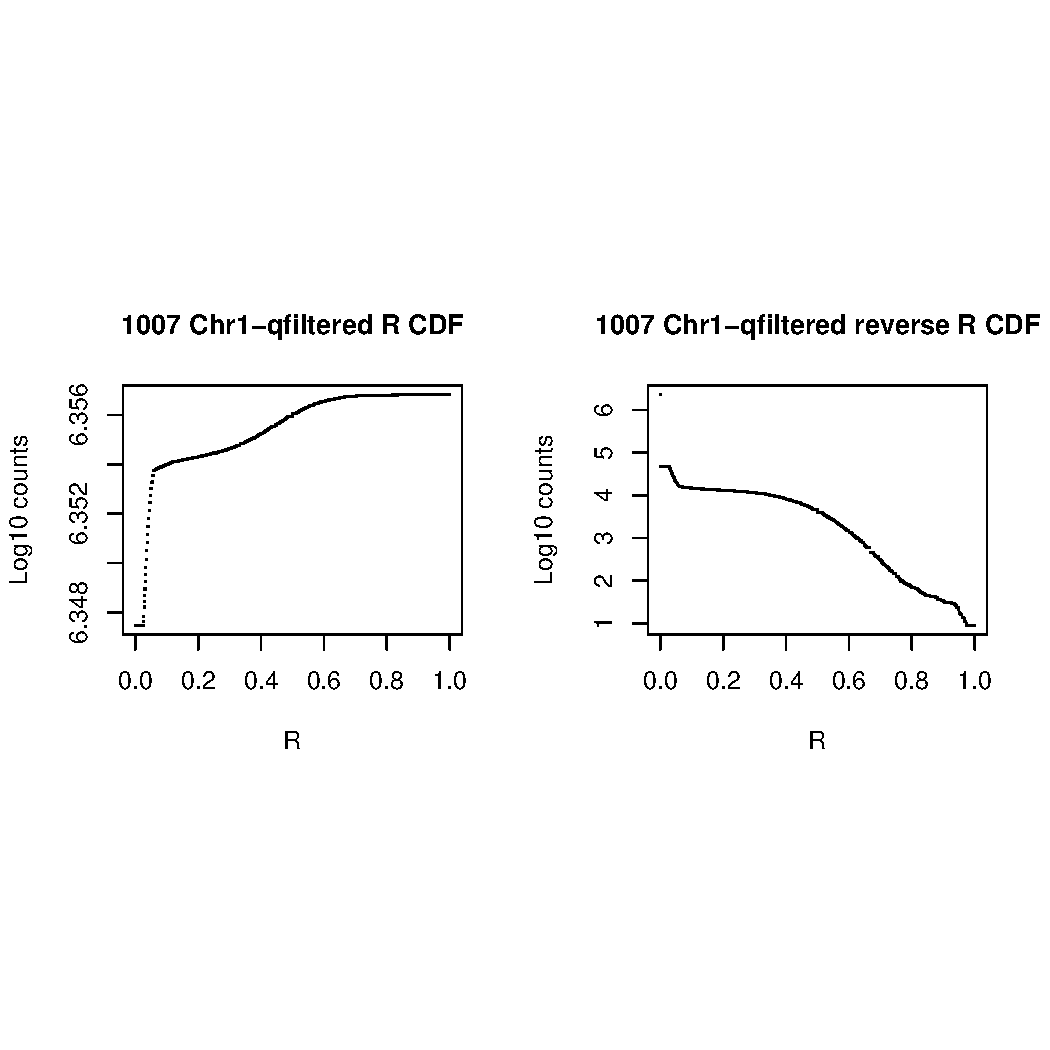
\includegraphics[width=\maxwidth]{FigS7-hwe-histo-figs-knitr/unnamed-chunk-10-44} 
\begin{kframe}\begin{verbatim}
#      [,1]    [,2]    [,3]    [,4]    [,5]  [,6]    [,7]    [,8]     [,9]     [,10]    [,11] 
# [1,] "blue"  "nm3"   "nm3x"  "nm3hi" "red" "black" "green" "orange" "ornghi" "nzgrey" "grey"
# [2,] "15649" "13349" "26698" "61"    NA    NA      NA      "26698"  "61"     NA       NA    
# FigS7-hwe-histo-figs-mine/S7-Chr1-qfiltered-1012.pdf written; 301-bin histo follows:
\end{verbatim}
\end{kframe}
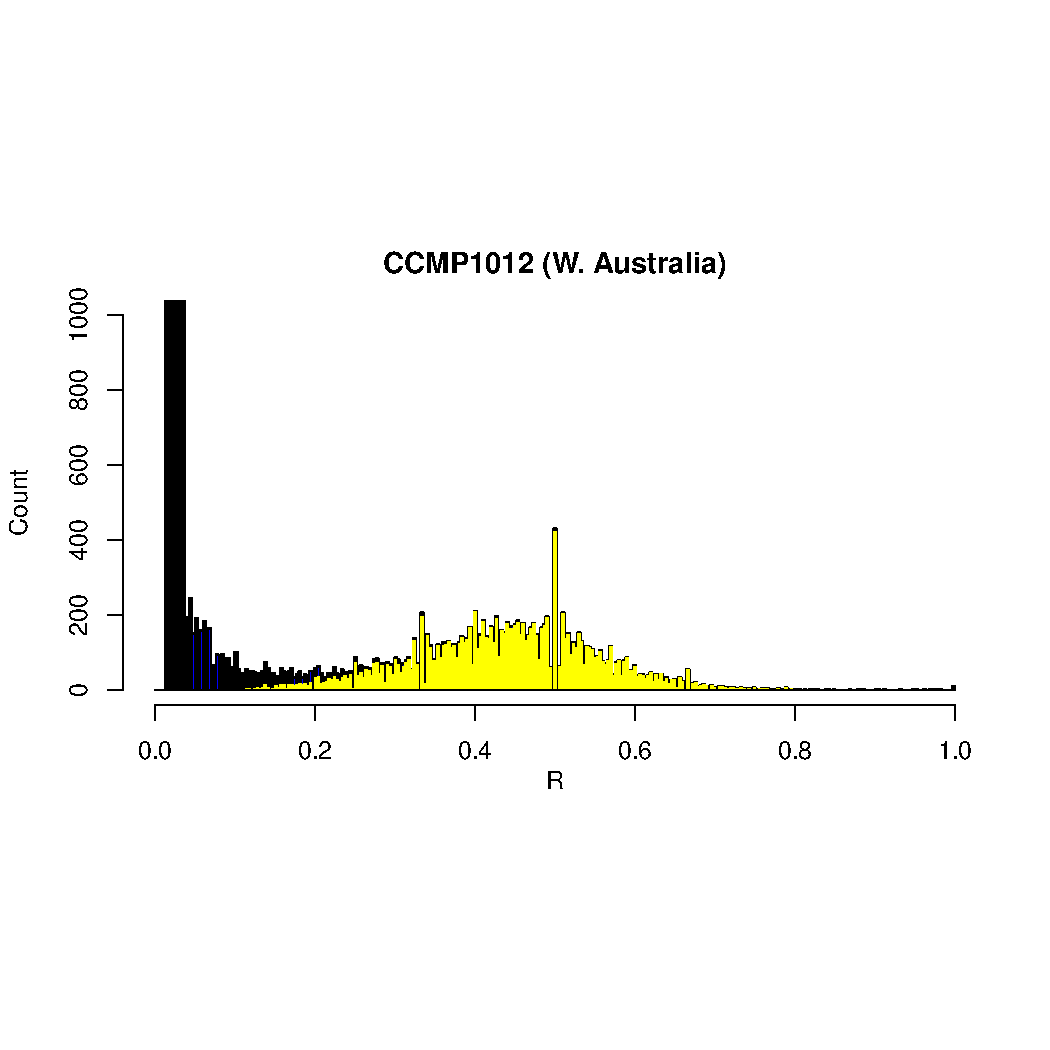
\includegraphics[width=\maxwidth]{FigS7-hwe-histo-figs-knitr/unnamed-chunk-10-45} 
\begin{kframe}\begin{verbatim}
#      [,1]    [,2]    [,3]   [,4]    [,5]  [,6]    [,7]    [,8]     [,9]     [,10]    [,11] 
# [1,] "blue"  "nm3"   "nm3x" "nm3hi" "red" "black" "green" "orange" "ornghi" "nzgrey" "grey"
# [2,] "15649" "14760" NA     "0"     NA    NA      NA      NA       NA       NA       NA
# 
# homnr:het ratios vs mod.humpth lo x hi, Chr1-qfiltered :
#       hi
# lo          0.7     0.75     0.76     0.77     0.78     0.79      0.8     0.85      0.9
#   0.1  88.50617 167.6047 182.5443 209.1449 236.7049 272.5849 314.2174 401.7778 452.1250
#   0.15 84.19753 159.4884 173.7089 199.0290 225.2623 259.4151 299.0435 382.3889 430.3125
#   0.16 83.46296 158.1047 172.2025 197.3043 223.3115 257.1698 296.4565 379.0833 426.5938
#   0.17 82.75309 156.7674 170.7468 195.6377 221.4262 255.0000 293.9565 375.8889 423.0000
#   0.18 81.81481 155.0000 168.8228 193.4348 218.9344 252.1321 290.6522 371.6667 418.2500
#   0.19 81.14815 153.7442 167.4557 191.8696 217.1639 250.0943 288.3043 368.6667 414.8750
#   0.2  80.29630 152.1395 165.7089 189.8696 214.9016 247.4906 285.3043 364.8333 410.5625
#   0.25 76.10494 144.2442 157.1139 180.0290 203.7705 234.6792 270.5435 345.9722 389.3438
# 
# 
# 1013 coverage summary for retained sites:
#    Min. 1st Qu.  Median    Mean 3rd Qu.    Max. 
#   22.00   32.00   40.00   40.91   49.00   64.00 
# FigS7-hwe-histo-figs-mine/S7-Chr1-qfiltered-1013.pdf :
#   based on 2396614 positions with coverage in [ 21.72348 , 64.73525 ]
\end{verbatim}
\end{kframe}
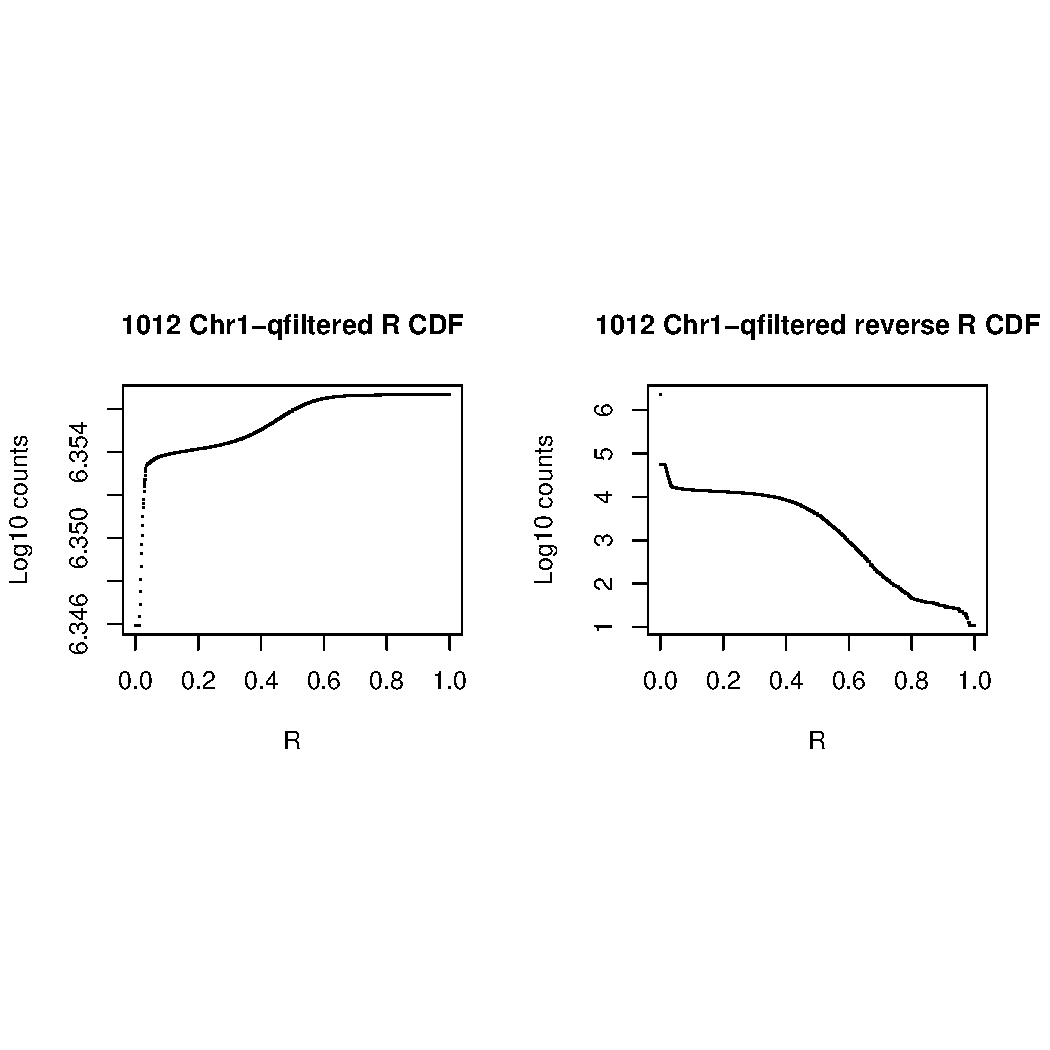
\includegraphics[width=\maxwidth]{FigS7-hwe-histo-figs-knitr/unnamed-chunk-10-46} 
\begin{kframe}\begin{verbatim}
#      [,1]    [,2]    [,3]    [,4]    [,5]  [,6]    [,7]    [,8]     [,9]     [,10]    [,11] 
# [1,] "blue"  "nm3"   "nm3x"  "nm3hi" "red" "black" "green" "orange" "ornghi" "nzgrey" "grey"
# [2,] "27960" "16457" "32914" "8308"  NA    NA      NA      "32914"  "8308"   NA       NA    
# FigS7-hwe-histo-figs-mine/S7-Chr1-qfiltered-1013.pdf written; 301-bin histo follows:
\end{verbatim}
\end{kframe}
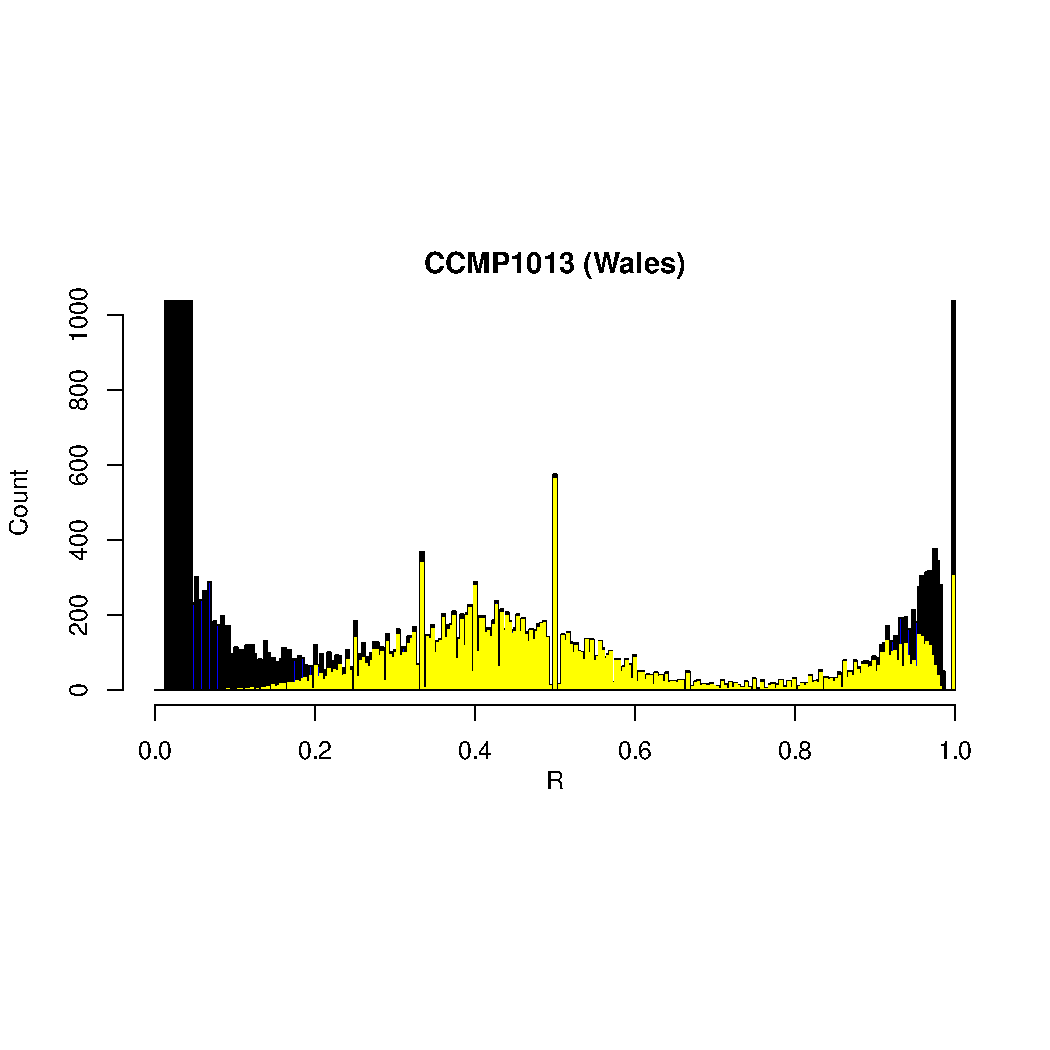
\includegraphics[width=\maxwidth]{FigS7-hwe-histo-figs-knitr/unnamed-chunk-10-47} 
\begin{kframe}\begin{verbatim}
#      [,1]    [,2]    [,3]   [,4]    [,5]  [,6]    [,7]    [,8]     [,9]     [,10]    [,11] 
# [1,] "blue"  "nm3"   "nm3x" "nm3hi" "red" "black" "green" "orange" "ornghi" "nzgrey" "grey"
# [2,] "27960" "18578" NA     "0"     NA    NA      NA      NA       NA       NA       NA
# 
# homnr:het ratios vs mod.humpth lo x hi, Chr1-qfiltered :
#       hi
# lo          0.7     0.75     0.76     0.77     0.78     0.79      0.8     0.85      0.9
#   0.1  2.110323 2.183603 2.195390 2.204575 2.219615 2.237928 2.262009 2.405677 2.823235
#   0.15 1.963497 2.033317 2.044548 2.053300 2.067629 2.085078 2.108022 2.244908 2.642755
#   0.16 1.934434 2.003570 2.014690 2.023356 2.037545 2.054823 2.077542 2.213086 2.607031
#   0.17 1.911183 1.979772 1.990804 1.999401 2.013478 2.030618 2.053158 2.187627 2.578451
#   0.18 1.882818 1.950738 1.961662 1.970176 1.984116 2.001089 2.023409 2.156568 2.543584
#   0.19 1.856196 1.923489 1.934313 1.942748 1.956558 1.973375 1.995489 2.127419 2.510860
#   0.2  1.826436 1.893027 1.903738 1.912085 1.925752 1.942394 1.964277 2.094832 2.474278
#   0.25 1.691002 1.754403 1.764601 1.772548 1.785560 1.801404 1.822238 1.946538 2.307802
# 
# 
# 1014 coverage summary for retained sites:
#    Min. 1st Qu.  Median    Mean 3rd Qu.    Max. 
#    6.00    8.00   11.00   11.54   14.00   19.00 
# FigS7-hwe-histo-figs-mine/S7-Chr1-qfiltered-1014.pdf :
#   based on 2189214 positions with coverage in [ 5.073091 , 19.79088 ]
\end{verbatim}
\end{kframe}
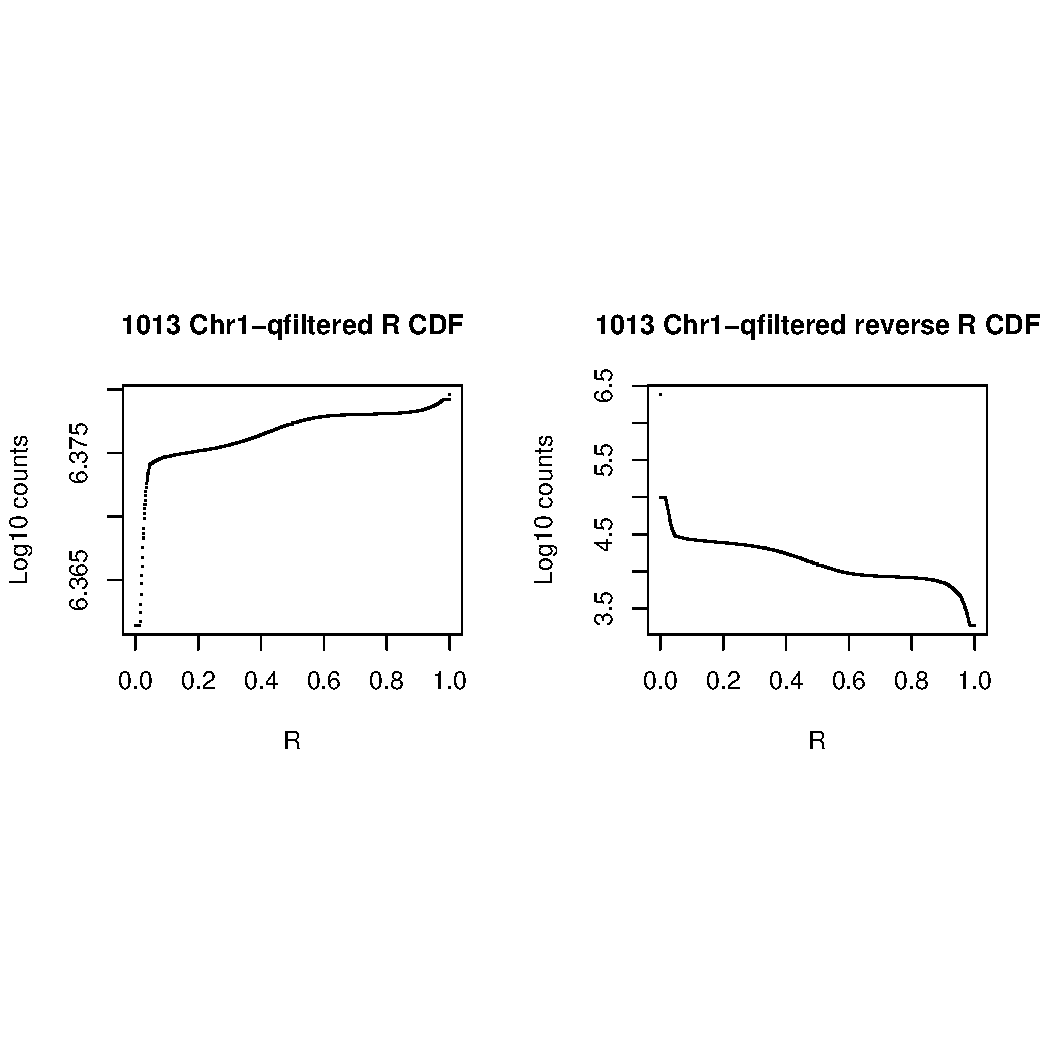
\includegraphics[width=\maxwidth]{FigS7-hwe-histo-figs-knitr/unnamed-chunk-10-48} 
\begin{kframe}\begin{verbatim}
#      [,1]   [,2]   [,3]    [,4]    [,5]  [,6]    [,7]    [,8]     [,9]     [,10]    [,11] 
# [1,] "blue" "nm3"  "nm3x"  "nm3hi" "red" "black" "green" "orange" "ornghi" "nzgrey" "grey"
# [2,] "8841" "8216" "16432" "427"   NA    NA      NA      "16432"  "427"    NA       NA    
# FigS7-hwe-histo-figs-mine/S7-Chr1-qfiltered-1014.pdf written; 301-bin histo follows:
\end{verbatim}
\end{kframe}
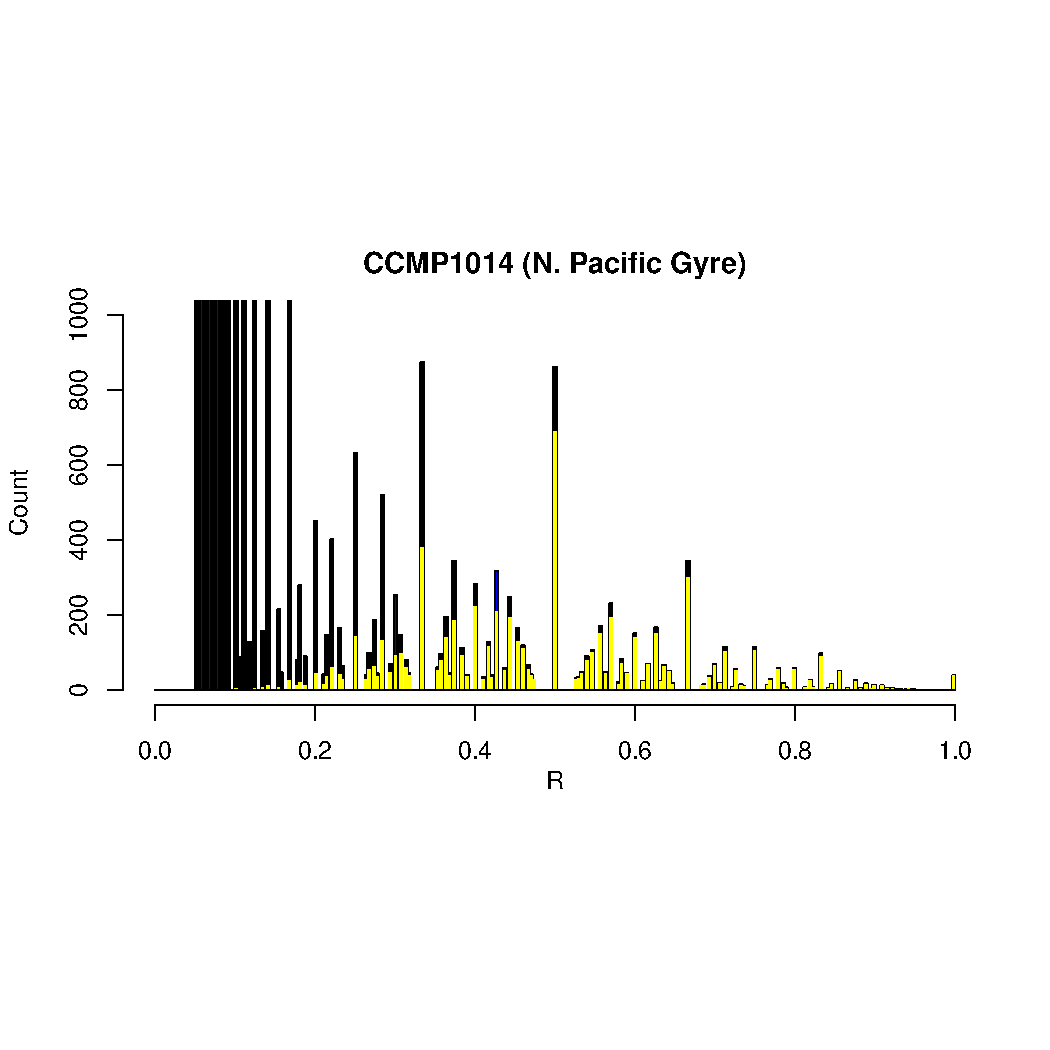
\includegraphics[width=\maxwidth]{FigS7-hwe-histo-figs-knitr/unnamed-chunk-10-49} 
\begin{kframe}\begin{verbatim}
#      [,1]   [,2]   [,3]   [,4]    [,5]  [,6]    [,7]    [,8]     [,9]     [,10]    [,11] 
# [1,] "blue" "nm3"  "nm3x" "nm3hi" "red" "black" "green" "orange" "ornghi" "nzgrey" "grey"
# [2,] "8841" "7085" NA     "0"     NA    NA      NA      NA       NA       NA       NA
# 
# homnr:het ratios vs mod.humpth lo x hi, Chr1-qfiltered :
#       hi
# lo           0.7     0.75     0.76     0.77     0.78     0.79      0.8      0.85      0.9
#   0.1  29.892202 49.92250 49.92250 54.31417 61.93925 65.51358 76.85549 142.28723 383.8286
#   0.15 15.746560 26.60491 26.60491 28.98563 33.11916 35.05679 41.20520  76.67553 207.6143
#   0.16 15.423165 26.07183 26.07183 28.40657 32.46028 34.36049 40.39017  75.17553 203.5857
#   0.17 11.568807 19.71834 19.71834 21.50513 24.60748 26.06173 30.67630  57.29787 155.5714
#   0.18 11.477064 19.56711 19.56711 21.34086 24.42056 25.86420 30.44509  56.87234 154.4286
#   0.19 11.016055 18.80718 18.80718 20.51540 23.48131 24.87160 29.28324  54.73404 148.6857
#   0.2  10.489679 17.93951 17.93951 19.57290 22.40888 23.73827 27.95665  52.29255 142.1286
#   0.25  8.769495 15.10397 15.10397 16.49281 18.90421 20.03457 23.62139  44.31383 120.7000
# 
# 
# 1015 coverage summary for retained sites:
#    Min. 1st Qu.  Median    Mean 3rd Qu.    Max. 
#   28.00   38.00   45.00   45.61   53.00   66.00 
# FigS7-hwe-histo-figs-mine/S7-Chr1-qfiltered-1015.pdf :
#   based on 2328577 positions with coverage in [ 27.627 , 66.34795 ]
\end{verbatim}
\end{kframe}
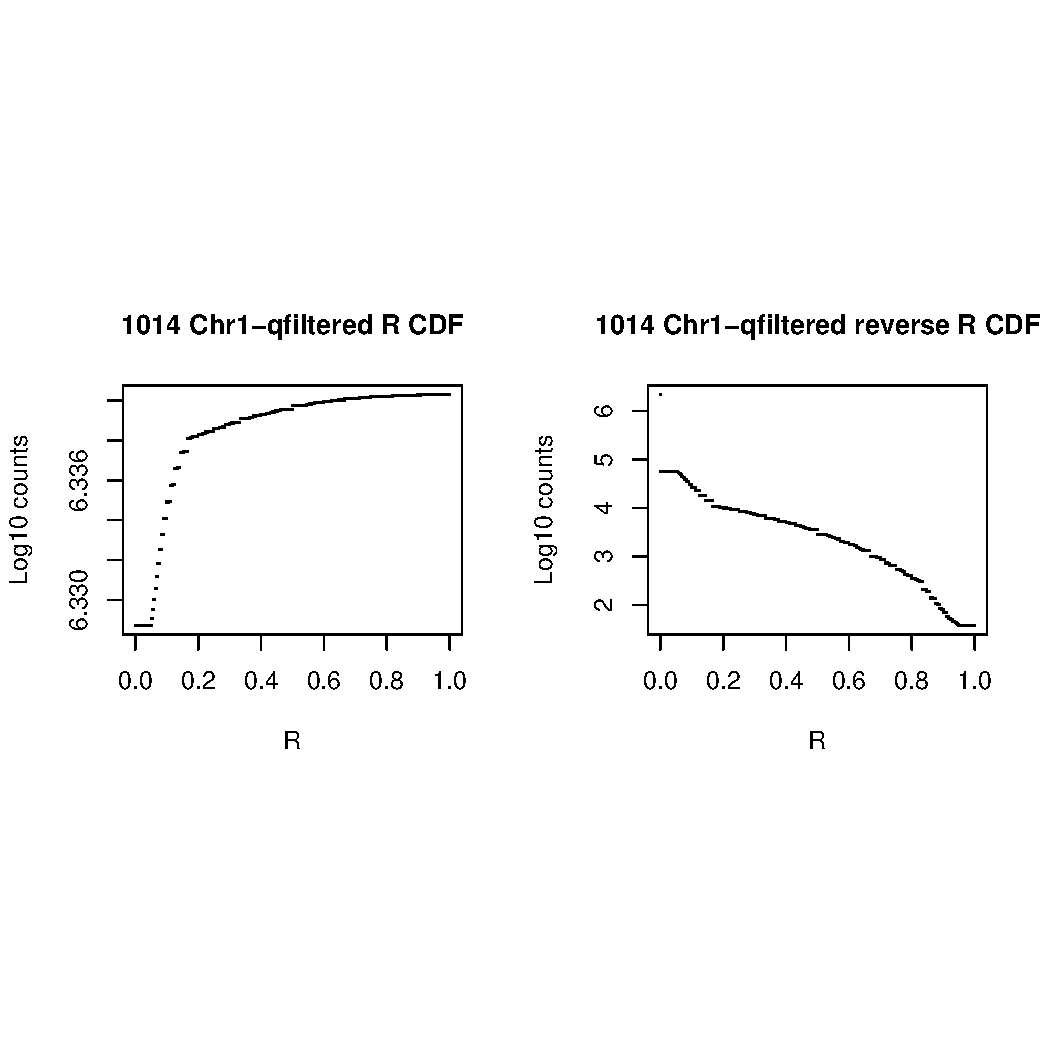
\includegraphics[width=\maxwidth]{FigS7-hwe-histo-figs-knitr/unnamed-chunk-10-50} 
\begin{kframe}\begin{verbatim}
#      [,1]    [,2]    [,3]    [,4]    [,5]  [,6]    [,7]    [,8]     [,9]     [,10]    [,11] 
# [1,] "blue"  "nm3"   "nm3x"  "nm3hi" "red" "black" "green" "orange" "ornghi" "nzgrey" "grey"
# [2,] "16261" "13992" "27984" "55"    NA    NA      NA      "27984"  "55"     NA       NA    
# FigS7-hwe-histo-figs-mine/S7-Chr1-qfiltered-1015.pdf written; 301-bin histo follows:
\end{verbatim}
\end{kframe}
\includegraphics[width=\maxwidth]{FigS7-hwe-histo-figs-knitr/unnamed-chunk-10-51} 
\begin{kframe}\begin{verbatim}
#      [,1]    [,2]    [,3]   [,4]    [,5]  [,6]    [,7]    [,8]     [,9]     [,10]    [,11] 
# [1,] "blue"  "nm3"   "nm3x" "nm3hi" "red" "black" "green" "orange" "ornghi" "nzgrey" "grey"
# [2,] "16261" "15235" NA     "0"     NA    NA      NA      NA       NA       NA       NA
# 
# homnr:het ratios vs mod.humpth lo x hi, Chr1-qfiltered :
#       hi
# lo          0.7     0.75     0.76     0.77     0.78   0.79      0.8     0.85      0.9
#   0.1  79.26596 202.9189 234.7812 259.1724 273.3636 300.80 349.9302 537.9286 684.9091
#   0.15 75.52660 193.4189 223.7969 247.0517 260.5818 286.74 333.5814 512.8214 652.9545
#   0.16 75.07979 192.2838 222.4844 245.6034 259.0545 285.06 331.6279 509.8214 649.1364
#   0.17 74.57979 191.0135 221.0156 243.9828 257.3455 283.18 329.4419 506.4643 644.8636
#   0.18 73.78191 188.9865 218.6719 241.3966 254.6182 280.18 325.9535 501.1071 638.0455
#   0.19 73.21277 187.5405 217.0000 239.5517 252.6727 278.04 323.4651 497.2857 633.1818
#   0.2  72.56383 185.8919 215.0938 237.4483 250.4545 275.60 320.6279 492.9286 627.6364
#   0.25 69.18085 177.2973 205.1562 226.4828 238.8909 262.88 305.8372 470.2143 598.7273
# 
# 
# 3367 coverage summary for retained sites:
#    Min. 1st Qu.  Median    Mean 3rd Qu.    Max. 
#   25.00   35.00   43.00   42.99   51.00   62.00 
# FigS7-hwe-histo-figs-mine/S7-Chr1-qfiltered-3367.pdf :
#   based on 2363450 positions with coverage in [ 24.65183 , 62.22891 ]
\end{verbatim}
\end{kframe}
\includegraphics[width=\maxwidth]{FigS7-hwe-histo-figs-knitr/unnamed-chunk-10-52} 
\begin{kframe}\begin{verbatim}
#      [,1]    [,2]    [,3]    [,4]    [,5]  [,6]    [,7]    [,8]     [,9]     [,10]    [,11] 
# [1,] "blue"  "nm3"   "nm3x"  "nm3hi" "red" "black" "green" "orange" "ornghi" "nzgrey" "grey"
# [2,] "24955" "13659" "27318" "8744"  NA    NA      NA      "27318"  "8744"   NA       NA    
# FigS7-hwe-histo-figs-mine/S7-Chr1-qfiltered-3367.pdf written; 301-bin histo follows:
\end{verbatim}
\end{kframe}
\includegraphics[width=\maxwidth]{FigS7-hwe-histo-figs-knitr/unnamed-chunk-10-53} 
\begin{kframe}\begin{verbatim}
#      [,1]    [,2]    [,3]   [,4]    [,5]  [,6]    [,7]    [,8]     [,9]     [,10]    [,11] 
# [1,] "blue"  "nm3"   "nm3x" "nm3hi" "red" "black" "green" "orange" "ornghi" "nzgrey" "grey"
# [2,] "24955" "15296" NA     "0"     NA    NA      NA      NA       NA       NA       NA
# 
# homnr:het ratios vs mod.humpth lo x hi, Chr1-qfiltered :
#       hi
# lo          0.7     0.75     0.76     0.77     0.78     0.79      0.8     0.85      0.9
#   0.1  1.653125 1.694016 1.702899 1.710295 1.717421 1.724897 1.743767 1.836416 2.162011
#   0.15 1.555469 1.594855 1.603411 1.610535 1.617398 1.624599 1.642775 1.732013 2.045624
#   0.16 1.533929 1.572983 1.581467 1.588530 1.595336 1.602476 1.620499 1.708985 2.019952
#   0.17 1.518973 1.557797 1.566231 1.573253 1.580018 1.587116 1.605032 1.692996 2.002128
#   0.18 1.501451 1.540005 1.548380 1.555353 1.562071 1.569120 1.586911 1.674263 1.981245
#   0.19 1.485156 1.523459 1.531779 1.538707 1.545382 1.552384 1.570060 1.656843 1.961825
#   0.2  1.462946 1.500907 1.509153 1.516019 1.522634 1.529574 1.547091 1.633099 1.935355
#   0.25 1.360826 1.397212 1.405117 1.411698 1.418038 1.424691 1.441482 1.523923 1.813647
# 
# 
# 1335 coverage summary for retained sites:
#    Min. 1st Qu.  Median    Mean 3rd Qu.    Max. 
#   50.00   67.00   80.00   79.43   92.00  108.00 
# FigS7-hwe-histo-figs-mine/S7-Chr1-qfiltered-1335.pdf :
#   based on 2253023 positions with coverage in [ 49.01378 , 108.5442 ]
\end{verbatim}
\end{kframe}
\includegraphics[width=\maxwidth]{FigS7-hwe-histo-figs-knitr/unnamed-chunk-10-54} 
\begin{kframe}\begin{verbatim}
#      [,1]    [,2]    [,3]    [,4]    [,5]  [,6]    [,7]    [,8]     [,9]     [,10]    [,11] 
# [1,] "blue"  "nm3"   "nm3x"  "nm3hi" "red" "black" "green" "orange" "ornghi" "nzgrey" "grey"
# [2,] "14482" "11741" "23482" "24"    NA    NA      NA      "23482"  "24"     NA       NA    
# FigS7-hwe-histo-figs-mine/S7-Chr1-qfiltered-1335.pdf written; 301-bin histo follows:
\end{verbatim}
\end{kframe}
\includegraphics[width=\maxwidth]{FigS7-hwe-histo-figs-knitr/unnamed-chunk-10-55} 
\begin{kframe}\begin{verbatim}
#      [,1]    [,2]    [,3]   [,4]    [,5]  [,6]    [,7]    [,8]     [,9]     [,10]    [,11] 
# [1,] "blue"  "nm3"   "nm3x" "nm3hi" "red" "black" "green" "orange" "ornghi" "nzgrey" "grey"
# [2,] "14482" "13973" NA     "0"     NA    NA      NA      NA       NA       NA       NA
\end{verbatim}
\end{kframe}
\includegraphics[width=\maxwidth]{FigS7-hwe-histo-figs-knitr/unnamed-chunk-10-56} 
\begin{kframe}\begin{verbatim}
# 
# homnr:het ratios vs mod.humpth lo x hi, Chr1-qfiltered :
#       hi
# lo          0.7     0.75     0.76     0.77     0.78   0.79      0.8   0.85     0.9
#   0.1  146.5349 332.8947 408.2903 487.0000 527.6667 633.40 844.8667 1267.8 3171.00
#   0.15 139.6163 317.2368 389.0968 464.1154 502.8750 603.65 805.2000 1208.3 3022.25
#   0.16 138.2791 314.2105 385.3871 459.6923 498.0833 597.90 797.5333 1196.8 2993.50
#   0.17 137.0814 311.5000 382.0645 455.7308 493.7917 592.75 790.6667 1186.5 2967.75
#   0.18 135.7791 308.5526 378.4516 451.4231 489.1250 587.15 783.2000 1175.3 2939.75
#   0.19 134.5930 305.8684 375.1613 447.5000 484.8750 582.05 776.4000 1165.1 2914.25
#   0.2  133.0581 302.3947 370.9032 442.4231 479.3750 575.45 767.6000 1151.9 2881.25
#   0.25 124.8953 283.9211 348.2581 415.4231 450.1250 540.35 720.8000 1081.7 2705.75
\end{verbatim}
\end{kframe}
\end{knitrout}

\begin{knitrout}\footnotesize
\definecolor{shadecolor}{rgb}{0.969, 0.969, 0.969}\color{fgcolor}\begin{kframe}
\begin{alltt}
\hlstd{tex.show.figs} \hlkwb{<-} \hlkwa{function}\hlstd{(}\hlkwc{fig.names}\hlstd{)\{}
  \hlcom{# quick hack to latex the figs, two per line.}
  \hlcom{# goal is to return a string something like this for each pair:}
  \hlcom{#}
  \hlcom{# \textbackslash{}par\textbackslash{}noindent fig.names[1], fig.names[2]:}
  \hlcom{#}
  \hlcom{# \textbackslash{}noindent\textbackslash{}includegraphics[width=.5\textbackslash{}linewidth]\{\textbackslash{}Sexpr\{fig.names[1]\}\}}
  \hlcom{# \textbackslash{}noindent\textbackslash{}includegraphics[width=.5\textbackslash{}linewidth]\{\textbackslash{}Sexpr\{fig.names[2]\}\}}

  \hlstd{npairs} \hlkwb{<-} \hlkwd{ceiling}\hlstd{(}\hlkwd{length}\hlstd{(fig.names)}\hlopt{/}\hlnum{2}\hlstd{)}
  \hlstd{texstr} \hlkwb{<-} \hlkwd{character}\hlstd{(npairs)}
  \hlkwa{for}\hlstd{(i} \hlkwa{in} \hlnum{1}\hlopt{:}\hlstd{npairs)\{}
    \hlkwa{if}\hlstd{(}\hlopt{!}\hlkwd{is.na}\hlstd{(fig.names[}\hlnum{2}\hlopt{*}\hlstd{i]))\{}
      \hlstd{texstr[i]} \hlkwb{<-} \hlkwd{paste}\hlstd{(}\hlstr{'\textbackslash{}\textbackslash{}par\textbackslash{}\textbackslash{}noindent '}\hlstd{, fig.names[}\hlnum{2}\hlopt{*}\hlstd{i}\hlopt{-}\hlnum{1}\hlstd{],} \hlstr{', '}\hlstd{, fig.names[}\hlnum{2}\hlopt{*}\hlstd{i],} \hlstr{':\textbackslash{}n\textbackslash{}n'}\hlstd{,}
                         \hlstr{'\textbackslash{}\textbackslash{}noindent\textbackslash{}\textbackslash{}includegraphics[width=.5\textbackslash{}\textbackslash{}linewidth]\{'}\hlstd{, fig.names[}\hlnum{2}\hlopt{*}\hlstd{i}\hlopt{-}\hlnum{1}\hlstd{],} \hlstr{'\}\textbackslash{}n'}\hlstd{,}
                         \hlstr{'\textbackslash{}\textbackslash{}noindent\textbackslash{}\textbackslash{}includegraphics[width=.5\textbackslash{}\textbackslash{}linewidth]\{'}\hlstd{, fig.names[}\hlnum{2}\hlopt{*}\hlstd{i],} \hlstr{'\}\textbackslash{}n'}\hlstd{,}
                         \hlkwc{sep}\hlstd{=}\hlstr{''}\hlstd{)}
    \hlstd{\}} \hlkwa{else} \hlstd{\{}
      \hlstd{texstr[i]} \hlkwb{<-} \hlkwd{paste}\hlstd{(}\hlstr{'\textbackslash{}\textbackslash{}par\textbackslash{}\textbackslash{}noindent '}\hlstd{, fig.names[}\hlnum{2}\hlopt{*}\hlstd{i}\hlopt{-}\hlnum{1}\hlstd{],} \hlstr{':\textbackslash{}n\textbackslash{}n'}\hlstd{,}
                         \hlstr{'\textbackslash{}\textbackslash{}noindent\textbackslash{}\textbackslash{}includegraphics[width=.5\textbackslash{}\textbackslash{}linewidth]\{'}\hlstd{, fig.names[}\hlnum{2}\hlopt{*}\hlstd{i}\hlopt{-}\hlnum{1}\hlstd{],} \hlstr{'\}\textbackslash{}n'}\hlstd{,}
                         \hlkwc{sep}\hlstd{=}\hlstr{''}\hlstd{)}

    \hlstd{\}}
  \hlstd{\}}
  \hlkwd{return}\hlstd{(}\hlkwd{paste}\hlstd{(texstr,}\hlkwc{collapse}\hlstd{=}\hlstr{'\textbackslash{}n'}\hlstd{))}
\hlstd{\}}
\end{alltt}
\end{kframe}
\end{knitrout}

\par\noindent FigS7-hwe-histo-figs-mine/S7-full-unfiltered-1007chronly.pdf, FigS7-hwe-histo-figs-mine/S7-full-unfiltered-1012chronly.pdf:

\noindent\includegraphics[width=.5\linewidth]{FigS7-hwe-histo-figs-mine/S7-full-unfiltered-1007chronly.pdf}
\noindent\includegraphics[width=.5\linewidth]{FigS7-hwe-histo-figs-mine/S7-full-unfiltered-1012chronly.pdf}

\par\noindent FigS7-hwe-histo-figs-mine/S7-full-unfiltered-1013chronly.pdf, FigS7-hwe-histo-figs-mine/S7-full-unfiltered-1014chronly.pdf:

\noindent\includegraphics[width=.5\linewidth]{FigS7-hwe-histo-figs-mine/S7-full-unfiltered-1013chronly.pdf}
\noindent\includegraphics[width=.5\linewidth]{FigS7-hwe-histo-figs-mine/S7-full-unfiltered-1014chronly.pdf}

\par\noindent FigS7-hwe-histo-figs-mine/S7-full-unfiltered-1015chronly.pdf, FigS7-hwe-histo-figs-mine/S7-full-unfiltered-3367chronly.pdf:

\noindent\includegraphics[width=.5\linewidth]{FigS7-hwe-histo-figs-mine/S7-full-unfiltered-1015chronly.pdf}
\noindent\includegraphics[width=.5\linewidth]{FigS7-hwe-histo-figs-mine/S7-full-unfiltered-3367chronly.pdf}

\par\noindent FigS7-hwe-histo-figs-mine/S7-full-unfiltered-1335chronly.pdf, FigS7-hwe-histo-figs-mine/S7-Chr1-unfiltered-1007.pdf:

\noindent\includegraphics[width=.5\linewidth]{FigS7-hwe-histo-figs-mine/S7-full-unfiltered-1335chronly.pdf}
\noindent\includegraphics[width=.5\linewidth]{FigS7-hwe-histo-figs-mine/S7-Chr1-unfiltered-1007.pdf}

\par\noindent FigS7-hwe-histo-figs-mine/S7-Chr1-unfiltered-1012.pdf, FigS7-hwe-histo-figs-mine/S7-Chr1-unfiltered-1013.pdf:

\noindent\includegraphics[width=.5\linewidth]{FigS7-hwe-histo-figs-mine/S7-Chr1-unfiltered-1012.pdf}
\noindent\includegraphics[width=.5\linewidth]{FigS7-hwe-histo-figs-mine/S7-Chr1-unfiltered-1013.pdf}

\par\noindent FigS7-hwe-histo-figs-mine/S7-Chr1-unfiltered-1014.pdf, FigS7-hwe-histo-figs-mine/S7-Chr1-unfiltered-1015.pdf:

\noindent\includegraphics[width=.5\linewidth]{FigS7-hwe-histo-figs-mine/S7-Chr1-unfiltered-1014.pdf}
\noindent\includegraphics[width=.5\linewidth]{FigS7-hwe-histo-figs-mine/S7-Chr1-unfiltered-1015.pdf}

\par\noindent FigS7-hwe-histo-figs-mine/S7-Chr1-unfiltered-3367.pdf, FigS7-hwe-histo-figs-mine/S7-Chr1-unfiltered-1335.pdf:

\noindent\includegraphics[width=.5\linewidth]{FigS7-hwe-histo-figs-mine/S7-Chr1-unfiltered-3367.pdf}
\noindent\includegraphics[width=.5\linewidth]{FigS7-hwe-histo-figs-mine/S7-Chr1-unfiltered-1335.pdf}

\par\noindent FigS7-hwe-histo-figs-mine/S7-full-qfiltered-1007chronly.pdf, FigS7-hwe-histo-figs-mine/S7-full-qfiltered-1012chronly.pdf:

\noindent\includegraphics[width=.5\linewidth]{FigS7-hwe-histo-figs-mine/S7-full-qfiltered-1007chronly.pdf}
\noindent\includegraphics[width=.5\linewidth]{FigS7-hwe-histo-figs-mine/S7-full-qfiltered-1012chronly.pdf}

\par\noindent FigS7-hwe-histo-figs-mine/S7-full-qfiltered-1013chronly.pdf, FigS7-hwe-histo-figs-mine/S7-full-qfiltered-1014chronly.pdf:

\noindent\includegraphics[width=.5\linewidth]{FigS7-hwe-histo-figs-mine/S7-full-qfiltered-1013chronly.pdf}
\noindent\includegraphics[width=.5\linewidth]{FigS7-hwe-histo-figs-mine/S7-full-qfiltered-1014chronly.pdf}

\par\noindent FigS7-hwe-histo-figs-mine/S7-full-qfiltered-1015chronly.pdf, FigS7-hwe-histo-figs-mine/S7-full-qfiltered-3367chronly.pdf:

\noindent\includegraphics[width=.5\linewidth]{FigS7-hwe-histo-figs-mine/S7-full-qfiltered-1015chronly.pdf}
\noindent\includegraphics[width=.5\linewidth]{FigS7-hwe-histo-figs-mine/S7-full-qfiltered-3367chronly.pdf}

\par\noindent FigS7-hwe-histo-figs-mine/S7-full-qfiltered-1335chronly.pdf, FigS7-hwe-histo-figs-mine/S7-Chr1-qfiltered-1007.pdf:

\noindent\includegraphics[width=.5\linewidth]{FigS7-hwe-histo-figs-mine/S7-full-qfiltered-1335chronly.pdf}
\noindent\includegraphics[width=.5\linewidth]{FigS7-hwe-histo-figs-mine/S7-Chr1-qfiltered-1007.pdf}

\par\noindent FigS7-hwe-histo-figs-mine/S7-Chr1-qfiltered-1012.pdf, FigS7-hwe-histo-figs-mine/S7-Chr1-qfiltered-1013.pdf:

\noindent\includegraphics[width=.5\linewidth]{FigS7-hwe-histo-figs-mine/S7-Chr1-qfiltered-1012.pdf}
\noindent\includegraphics[width=.5\linewidth]{FigS7-hwe-histo-figs-mine/S7-Chr1-qfiltered-1013.pdf}

\par\noindent FigS7-hwe-histo-figs-mine/S7-Chr1-qfiltered-1014.pdf, FigS7-hwe-histo-figs-mine/S7-Chr1-qfiltered-1015.pdf:

\noindent\includegraphics[width=.5\linewidth]{FigS7-hwe-histo-figs-mine/S7-Chr1-qfiltered-1014.pdf}
\noindent\includegraphics[width=.5\linewidth]{FigS7-hwe-histo-figs-mine/S7-Chr1-qfiltered-1015.pdf}

\par\noindent FigS7-hwe-histo-figs-mine/S7-Chr1-qfiltered-3367.pdf, FigS7-hwe-histo-figs-mine/S7-Chr1-qfiltered-1335.pdf:

\noindent\includegraphics[width=.5\linewidth]{FigS7-hwe-histo-figs-mine/S7-Chr1-qfiltered-3367.pdf}
\noindent\includegraphics[width=.5\linewidth]{FigS7-hwe-histo-figs-mine/S7-Chr1-qfiltered-1335.pdf}


\section{R vs SAMtools SNP calls}
\label{sec:rvsam}

A quick tangent: How do SAMtools SNP calls correlate to R stats?  Code below makes a quick-and-dirty R histogram, overlaid with histo of number of SNP calls in each bin.  Short answer is that $\approx80\%$ of points in the middle hump are called SNPs by SAMtools and, in un-q-filtered data, $<25\%$ of points above $R=0.78$ are called SNPs.  At first glance, this seems like good discrimination of heterozygous from homozygous, but whether this is because SAMtools considered them to be homozygous, or because the alignment quality was low on average (or both) is unclear.  But the $25\%$ rises to $\approx50\%$ in q-filtered H-clade, which we believe to be homozygous nonreference.  (We did not re-run SAMtoold after q-filter.)  In short, mis-classification of homozygous non-reference as heterozygus may be a significant contributor to the large SNP-counts seen in H-clade.  

NOTE: After writing this code chunk, I modified code in the preceding section to add the analogous histo based on $\mu\pm\sigma$, etc. to the 301 bin plots, so those plots are more accurate, but the numerical summary below is still a useful ballpark.

\begin{knitrout}\footnotesize
\definecolor{shadecolor}{rgb}{0.969, 0.969, 0.969}\color{fgcolor}\begin{kframe}
\begin{alltt}
\hlstd{snp.vs.r} \hlkwb{<-} \hlkwa{function}\hlstd{(}\hlkwc{tables}\hlstd{,}\hlkwc{st}\hlstd{=}\hlnum{3}\hlstd{,}\hlkwc{breaks}\hlstd{=}\hlnum{41}\hlstd{,}\hlkwc{maxy}\hlstd{=}\hlnum{2000}\hlstd{,}\hlkwc{hump}\hlstd{=model.humpth)\{}
 \hlcom{#cov <- tables[[st]]$Cov}
  \hlstd{mat} \hlkwb{<-} \hlstd{tables[[st]]}\hlopt{$}\hlstd{.match}
  \hlstd{nr}  \hlkwb{<-} \hlkwd{pmax}\hlstd{(tables[[st]]}\hlopt{$}\hlstd{a,tables[[st]]}\hlopt{$}\hlstd{c,tables[[st]]}\hlopt{$}\hlstd{g,tables[[st]]}\hlopt{$}\hlstd{t)}
  \hlstd{r}   \hlkwb{<-} \hlstd{nr}\hlopt{/}\hlstd{(nr}\hlopt{+}\hlstd{mat)}
  \hlstd{snp} \hlkwb{<-}\hlstd{tables[[st]]}\hlopt{$}\hlstd{snp}
  \hlstd{aa} \hlkwb{<-} \hlkwd{hist}\hlstd{(r,}\hlkwc{ylim}\hlstd{=}\hlkwd{c}\hlstd{(}\hlnum{0}\hlstd{,maxy),}\hlkwc{breaks}\hlstd{=breaks,}\hlkwc{col}\hlstd{=}\hlstr{'blue'}\hlstd{)}
  \hlstd{bb} \hlkwb{<-} \hlkwd{hist}\hlstd{(r[snp}\hlopt{==}\hlnum{1}\hlstd{],}\hlkwc{ylim}\hlstd{=}\hlkwd{c}\hlstd{(}\hlnum{0}\hlstd{,maxy),}\hlkwc{breaks}\hlstd{=breaks,}\hlkwc{col}\hlstd{=}\hlstr{'yellow'}\hlstd{,}\hlkwc{add}\hlstd{=T)}
  \hlcom{#should use breaks not mids but this is easier:}
  \hlstd{df} \hlkwb{<-} \hlkwd{data.frame}\hlstd{(}
    \hlkwc{r.mid}   \hlstd{=} \hlkwd{sum}\hlstd{(aa}\hlopt{$}\hlstd{counts[hump[}\hlnum{1}\hlstd{]} \hlopt{<=} \hlstd{aa}\hlopt{$}\hlstd{mids} \hlopt{&} \hlstd{aa}\hlopt{$}\hlstd{mids} \hlopt{<=} \hlstd{hump[}\hlnum{2}\hlstd{]]),}
    \hlkwc{sam.mid} \hlstd{=} \hlkwd{sum}\hlstd{(bb}\hlopt{$}\hlstd{counts[hump[}\hlnum{1}\hlstd{]} \hlopt{<=} \hlstd{bb}\hlopt{$}\hlstd{mids} \hlopt{&} \hlstd{bb}\hlopt{$}\hlstd{mids} \hlopt{<=} \hlstd{hump[}\hlnum{2}\hlstd{]]),}
    \hlkwc{sam.over.r.mid} \hlstd{=} \hlnum{NA}\hlstd{,}
    \hlkwc{r.hi}   \hlstd{=} \hlkwd{sum}\hlstd{(aa}\hlopt{$}\hlstd{counts[hump[}\hlnum{2}\hlstd{]} \hlopt{<} \hlstd{aa}\hlopt{$}\hlstd{mids]),}
    \hlkwc{sam.hi} \hlstd{=} \hlkwd{sum}\hlstd{(bb}\hlopt{$}\hlstd{counts[hump[}\hlnum{2}\hlstd{]} \hlopt{<} \hlstd{bb}\hlopt{$}\hlstd{mids]),}
    \hlkwc{sam.over.r.hi} \hlstd{=} \hlnum{NA}\hlstd{,}
    \hlkwc{tables} \hlstd{=} \hlkwd{which.snp.tables}\hlstd{(tables),}
    \hlkwc{isolate} \hlstd{=} \hlkwd{st.loc}\hlstd{(st)}
  \hlstd{)}
  \hlstd{df}\hlopt{$}\hlstd{sam.over.r.mid} \hlkwb{<-} \hlstd{df}\hlopt{$}\hlstd{sam.mid}\hlopt{/}\hlstd{df}\hlopt{$}\hlstd{r.mid}
  \hlstd{df}\hlopt{$}\hlstd{sam.over.r.hi}  \hlkwb{<-} \hlstd{df}\hlopt{$}\hlstd{sam.hi} \hlopt{/}\hlstd{df}\hlopt{$}\hlstd{r.hi}
  \hlkwd{return}\hlstd{(df)}
\hlstd{\}}
\hlstd{all.df} \hlkwb{<-} \hlkwa{NULL}
\hlkwa{for}\hlstd{(tab} \hlkwa{in} \hlnum{1}\hlopt{:}\hlnum{4}\hlstd{)\{}
  \hlkwa{if}\hlstd{(}\hlopt{!}\hlkwd{is.null}\hlstd{(tset[[tab]]))\{}
    \hlstd{wst.full} \hlkwb{<-} \hlkwd{which.snp.tables}\hlstd{(}\hlkwc{tables}\hlstd{=tset[[tab]],} \hlkwc{string.val}\hlstd{=}\hlnum{FALSE}\hlstd{)[}\hlnum{1}\hlstd{]} \hlopt{==} \hlstr{'full'}
    \hlstd{temp3} \hlkwb{<-} \hlkwd{snp.vs.r}\hlstd{(tset[[tab]],}\hlnum{3}\hlstd{,}\hlkwc{maxy}\hlstd{=}\hlnum{2000}\hlopt{*}\hlkwd{ifelse}\hlstd{(wst.full,}\hlnum{10}\hlstd{,}\hlnum{1}\hlstd{))}
    \hlstd{temp6} \hlkwb{<-} \hlkwd{snp.vs.r}\hlstd{(tset[[tab]],}\hlnum{6}\hlstd{,}\hlkwc{maxy}\hlstd{=}\hlnum{2000}\hlopt{*}\hlkwd{ifelse}\hlstd{(wst.full,}\hlnum{10}\hlstd{,}\hlnum{1}\hlstd{))}
    \hlstd{all.df} \hlkwb{<-} \hlkwd{rbind}\hlstd{(all.df,temp3,temp6)}
  \hlstd{\}}
\hlstd{\}}
\end{alltt}
\end{kframe}
\includegraphics[width=\maxwidth]{FigS7-hwe-histo-figs-knitr/unnamed-chunk-12-1} 

\includegraphics[width=\maxwidth]{FigS7-hwe-histo-figs-knitr/unnamed-chunk-12-2} 

\includegraphics[width=\maxwidth]{FigS7-hwe-histo-figs-knitr/unnamed-chunk-12-3} 

\includegraphics[width=\maxwidth]{FigS7-hwe-histo-figs-knitr/unnamed-chunk-12-4} 

\includegraphics[width=\maxwidth]{FigS7-hwe-histo-figs-knitr/unnamed-chunk-12-5} 

\includegraphics[width=\maxwidth]{FigS7-hwe-histo-figs-knitr/unnamed-chunk-12-6} 

\includegraphics[width=\maxwidth]{FigS7-hwe-histo-figs-knitr/unnamed-chunk-12-7} 

\includegraphics[width=\maxwidth]{FigS7-hwe-histo-figs-knitr/unnamed-chunk-12-8} 
\begin{kframe}\begin{alltt}
\hlkwd{print}\hlstd{(all.df)}
\end{alltt}
\begin{verbatim}
#    r.mid sam.mid sam.over.r.mid   r.hi sam.hi sam.over.r.hi          tables          isolate
# 1 277374  235819      0.8501842  54194   7203     0.1329114 full-unfiltered CCMP1013 (Wales)
# 2 268898  224464      0.8347552  62045  13700     0.2208075 full-unfiltered CCMP3367 (Italy)
# 3  26785   23540      0.8788501   5243    765     0.1459088 Chr1-unfiltered CCMP1013 (Wales)
# 4  25535   22467      0.8798512   5829   1362     0.2336593 Chr1-unfiltered CCMP3367 (Italy)
# 5 249697  192064      0.7691883 121202  59071     0.4873764  full-qfiltered CCMP1013 (Wales)
# 6 222025  163357      0.7357595 144422  80614     0.5581837  full-qfiltered CCMP3367 (Italy)
# 7  23523   19151      0.8141394  11813   5971     0.5054601  Chr1-qfiltered CCMP1013 (Wales)
# 8  20717   16521      0.7974610  13589   7836     0.5766429  Chr1-qfiltered CCMP3367 (Italy)
\end{verbatim}
\begin{alltt}
\hlcom{# note that snp calls were not changed in q-filtered data.  E.g.:}
\hlkwa{if}\hlstd{(}\hlopt{!}\hlkwd{is.null}\hlstd{(tset[[}\hlnum{2}\hlstd{]])} \hlopt{&& !}\hlkwd{is.null}\hlstd{(tset[[}\hlnum{4}\hlstd{]]))\{}
  \hlkwd{print}\hlstd{(}\hlkwd{all}\hlstd{(tset[[}\hlnum{2}\hlstd{]][[}\hlnum{1}\hlstd{]]}\hlopt{$}\hlstd{snp} \hlopt{==} \hlstd{tset[[}\hlnum{4}\hlstd{]][[}\hlnum{1}\hlstd{]]}\hlopt{$}\hlstd{snp))}
\hlstd{\}}
\end{alltt}
\begin{verbatim}
# [1] TRUE
\end{verbatim}
\end{kframe}
\end{knitrout}

\section{The Specific S7 Figures}

These are the ones intended for Supp Fig S7, full size:

\noindent
\includegraphics{FigS7-hwe-histo-figs-mine/S7-full-qfiltered-1013chronly.pdf}\\
\includegraphics{FigS7-hwe-histo-figs-mine/S7-full-qfiltered-3367chronly.pdf}

\section{To Do/Improvements?}

I think the axis labels take up more space than is reasonable, would look better if a bit more 
compact.  The best resource I've seen on this is:
\href{http://www.carlislerainey.com/2012/12/17/controlling-axes-of-r-plots/}{http://www.carlislerainey.com/2012/12/17/controlling-axes-of-r-plots/} .
But not sure it's compatible with Histo, and would need work to plot 2-in-1.


% remember to do this to enable Id keyword substution: svn propset svn:keywords Id fig1b.rnw 
\vfill\footnotesize\flushright SVN Id, I miss you.\  $ $Id: 2017-07-12 or later. $ $
\end{document}
